%
%****************************************************************************************************
%=========================== B E G I N   S U B D O C U M E N T  ==========================
%****************************************************************************************************
%
\documentclass[a4paper, 12pt, xcolor=dvipsnames]{scrartcl}		% Article als Modul
\usepackage[ngerman]{babel}
\usepackage[onehalfspacing]{setspace}
\usepackage{fancyhdr}
\usepackage{xcolor}
\usepackage[utf8x]{inputenc}
\usepackage{wrapfig}
\usepackage{color}
\usepackage{acronym}
\usepackage{ifthen}
\usepackage{lastpage}
\usepackage{currfile}
\usepackage{caption}						% Formatierung der Bildunterschriften
\usepackage{sidecap}
\usepackage{subcaption}
\usepackage{tikz}
\usepackage{calc}
\usepackage{graphicx}
\usepackage{multirow}
\usepackage{longtable}
\usepackage{amsthm}
\usepackage{amsbsy}
\usepackage{geometry}
\usepackage{amssymb}
\usepackage{array}
\usepackage{chngpage}
\usepackage{tabulary} 					% instead of tabularx
\usepackage{array,longtable,calc,amsmath}
\usepackage{xspace}
\usepackage{pdfpages}
\usepackage{textfit}
\usepackage{tabu}
\usepackage{setspace}
\usepackage{listings}
\usepackage[T1]{fontenc}                  % Wichtig für korrekte Umlaute/Schriftkodierung
\usepackage[scaled]{helvet}												% Schriftart: Helvetica (Arial-Ersatz)
\renewcommand*\familydefault{\sfdefault}
\pagestyle{fancy}
\usepackage[acronym,toc]{glossaries}
\usepackage{docmute}				% includes parts of files just within the Begin and End Document
\usepackage[most]{tcolorbox}
\usepackage[hidelinks]{hyperref}	% Klickbare Links und URLs
\usepackage{url}					% URL-Formatierung

% --- Literaturverwaltung mit biblatex ---
\usepackage[
    backend=biber,
    style=alphabetic,
    sorting=nty,
    urldate=short
]{biblatex}


% Komma nach dem Autor statt Punkt im Verzeichnis
\DeclareDelimFormat{nametitledelim}{\addcomma\space}

% Titel im Verzeichnis nicht kursiv
\DeclareFieldFormat{title}{#1}

% "In: <URL>" statt "URL: <URL>"
\DeclareFieldFormat{url}{In:\space\url{#1}}

% "am <Datum>" statt "besucht am <Datum>"
\DefineBibliographyStrings{ngerman}{
  urlseen = {am},
}

\addbibresource{literatur.bib}
% ----------------------------------------

%---------------------Switch modulare Printversionen
%
\newboolean{UseWm} 		%Korrektur Wasserzeichen in das PDF drucken
\setboolean{UseWm}{false} 		%Zuweisung eines Wertes                    			% Input file für gemeinsame Package Definitionen
%
%--------------------Set data for document:
\newcommand{\SYear}{2025/26}
\newcommand{\SClass}{5AHIT}
\newcommand{\ADatum}{XX. April 2026}
\newcommand{\DAName}{Kennzeichenerkennungssystem Parkplatz Zotter}
\newcommand{\DPLNameOne}{Julian Bierbaum}
\newcommand{\DPLNameTwo}{}
\newcommand{\BNameOne}{DI (FH) Ing. Gerald Ebner}
\newcommand{\BNameTwo}{}
%
\newcommand{\WatermarkName}{}
%
\definecolor{green}{rgb}{0.8,1.0,0.2}
\definecolor{orange}{rgb}{0.9,0.64,0.25}
\definecolor{kaki}{rgb}{0.74,0.74,0.088}
\definecolor{blue}{rgb}{0.2,0.59,0.94}
\definecolor{dred}{rgb}{0.722,0.18,0.18}
\definecolor{itblue}{HTML}{102D69}

%
%------------------------------Watermark wird mit einer Designvariablen geladen ---------------------------------------------------------------------------------
%
\ifthenelse{\boolean{UseWm}}%
{\usepackage{draftwatermark}\SetWatermarkText{\WatermarkName$~-~$\WatermarkName\xspace$~-~$\WatermarkName} \SetWatermarkLightness{0.8}\SetWatermarkScale{2}}{}
%
\graphicspath{{./../03_AUX/01_PICT/}}
\newcommand{\changefont}[3]{\fontfamily{#1} \fontseries{#2} \fontshape{#3} \selectfont} % Change a new font 
% Weg mit der standard LATEX FONT

%
% --------------------Set the figure description:
%
\captionsetup{margin=10pt,font=small, labelfont={color=black!80, bf}, textfont={color=black!60}, format=hang, indention=-1cm}
\captionsetup[wrapfigure]{name=Bild}
\captionsetup[figure]{name=Bild}
% --------------------Set the page margins:
%
\setlength{\voffset}{0.0cm}
\setlength{\textwidth}{16.0cm}
%\addtolength{\textheight}{10.0cm}
\setlength{\textheight}{23.2cm}
\setlength{\topmargin }{-1.7cm}
\setlength{\marginparsep }{0pt}
\setlength{\headsep }{1.2cm}
\setlength{\oddsidemargin}{0.4cm}
\setlength{\evensidemargin}{0.4cm}
\setlength{\marginparwidth}{0pt}
\setlength{\hoffset}{-12pt}
\setlength{\headwidth}{16.0cm}
\setlength{\footskip}{35pt}
\setlength{\parindent}{0pt}
%
%

%--------------------Set environment for Header and and Footer:
%
\pagestyle{fancy}
\rhead{
\includegraphics[scale=0.07]{/HTL_logo.pdf}}
\chead{}
%\lhead{\begin{tabular}{p{7.0cm}} 
%		\small{\changefont{pag}{b}{sc}\textcolor{black!30}{\DAName}}
%	\end{tabular} \vspace{0.1cm}}
%\lfoot{\small{\changefont{pag}{b}{sc}\textcolor{black!30}{\SYear - \SClass - \DPLNameOne, \DPLNameTwo}}} 
%\cfoot{}
%\rfoot{\small{\changefont{pag}{b}{sc}\textcolor{black!30}{\thepage\ \textbf{\textcolor{orange!100}I} \pageref{LastPage}}}}
\lhead{\begin{tabular}{p{14.0cm}}
    \small{\sffamily\bfseries\textcolor{black!30}{\DAName}}
  \end{tabular} \vspace{0.1cm}}
\lfoot{\small{\sffamily\bfseries\textcolor{black!30}{\SYear - \SClass - \DPLNameOne \DPLNameTwo}}}
\cfoot{}
\rfoot{\small{\sffamily\bfseries\textcolor{black!30}{\thepage\ \textbf{\textcolor{blue!100}I} \pageref{LastPage}}}}
%s
\renewcommand{\headrulewidth}{0.4pt}
\renewcommand{\footrulewidth}{0.4pt}
\let\myHeadrule\headrule
\let\myFootrule\footrule
\renewcommand\headrule{\color{black!30}\myHeadrule }
\renewcommand\footrule{\color{black!30}\myFootrule }
\addto{\captionsngerman}{%
  \renewcommand*{\contentsname}{Inhalt}
  \renewcommand*{\listfigurename}{Abbildungen}
  \renewcommand*{\listtablename}{Abbildungsverzeichnis}
}
%\pagestyle{fancy}
%\fancypagestyle{ErsteSeite}{%
%	\fancyhf{}%
%	\fancyhead[L]{}
%}

\fancypagestyle{ErsteSeite}{%
  \fancyhf{}
  \renewcommand{\headrulewidth}{0.4pt}
  
  \fancyhead[C]{%
    \begin{minipage}[b]{0.2\textwidth}
      \raggedright
      
\includegraphics[width=\linewidth]{../../03_AUX/01_PICT/HTL-Weiz-Logo.pdf}
    \end{minipage}%
    \hfill
    \begin{minipage}[b]{0.65\textwidth}
      \centering
      \small 
      \textbf{Höhere Technische Bundeslehranstalt Weiz}\\[2pt]
      \footnotesize
      \textbf{Höhere Abteilung für Elektrotechnik}\\
      Ausbildungsschwerpunkt Informationstechnologie
    \end{minipage}%
    \hfill
    \begin{minipage}[b]{0.12\textwidth}
      \raggedleft
      
\includegraphics[width=\linewidth]{../../03_AUX/01_PICT/HTL-Weiz-IT-Logo.png}
    \end{minipage}%
    \vspace{2mm}
  }
  
  % Fußzeile für ErsteSeite
  
}
%\makenoidxglossaries
\renewcommand*\acronymname{Abkürzungsverzeichnis}
\renewcommand*\glossaryname{Glossar}

%--------------------Neue Umgebung für M E R K S A T Z (NEU) --------------------

% Zählerdefinition
\newcounter{MsNr}
\renewcommand{\theMsNr}{\arabic{MsNr}}

% Definition der Box mit tcolorbox
\newtcolorbox{Merksatz}{
  enhanced,              % Erlaubt Schatten
  colback=yellow!10,     % Hintergrundfarbe
  colframe=kaki,         % Rahmenfarbe
  boxrule=1pt,           % Rahmendicke
  arc=3pt,               % Eckenradius
  drop fuzzy shadow,     % Weicher Schatten
  width=15cm,            % Breite
  center,                % Zentriert die Box
  before upper={\refstepcounter{MsNr}\textcolor{kaki}{\large\textbf{Merke \theMsNr:}}~} % Titel
}
%--------------------------------------------------------------------------------

% --- Colors for Code Listings (Modern Theme) ---
\definecolor{codegreen}{rgb}{0.13, 0.55, 0.13}
\definecolor{codegray}{rgb}{0.5, 0.5, 0.5}
\definecolor{codepurple}{rgb}{0.58, 0, 0.82}
\definecolor{backcolour}{rgb}{0.96, 0.96, 0.96}
\definecolor{codeblue}{rgb}{0.16, 0.32, 0.75}

% Settings for Codelistings within documentation:
\lstset{ % General setup for the package
  language=C,
  backgroundcolor=\color{backcolour},
  basicstyle=\small\ttfamily\linespread{1}\selectfont,
  commentstyle=\color{codegreen}\itshape,
  keywordstyle=\color{codeblue}\bfseries,
  numberstyle=\tiny\color{codegray},
  stringstyle=\color{codepurple},
  numbers=left,
  numbersep=8pt,
  frame=single,
  rulecolor=\color{black!20},
  tabsize=4,
  columns=fullflexible,
  showstringspaces=false,
  showtabs=false,
  keepspaces=true,
  breaklines=true,
  breakatwhitespace=false,
  aboveskip=10pt,
  belowskip=10pt,
}

% --- Python Configuration ---
\lstdefinestyle{mypython}{
  language=Python,
  alsoletter={@},
  showstringspaces=false,
  morekeywords={access,and,break,class,continue,def,del,elif,else,except,exec,finally,for,from,global,if,import,in,is,lambda,not,or,pass,print,raise,return,try,while,assert,yield,async,await,True,False,None},
  keywordstyle=\color{codeblue}\bfseries,
  morekeywords=[2]{@app.post, @app.get, @app.put, @app.delete, @app.patch, @app.options, @app.head, @app.router, @router.post, @router.get, @router.put, @router.delete, @router.patch, @router.options, @router.head, Depends, HTTPException},
  keywordstyle=[2]\color{codepurple}\bfseries,
  emph={self,cls},
  emphstyle=\color{codepurple}\itshape,
}

% --- YAML Configuration ---
\newcommand\YAMLcolonstyle{\color{black}\mdseries}
\newcommand\YAMLkeystyle{\color{codeblue}\bfseries}
\newcommand\YAMLvaluestyle{\color{codepurple}\mdseries}

\makeatletter

\newcommand\language@yaml{yaml}

\expandafter\expandafter\expandafter\lstdefinelanguage
\expandafter{\language@yaml}
{
keywords={true,false,null,y,n},
keywordstyle=\color{darkgray}\bfseries,
basicstyle=\YAMLkeystyle\small\ttfamily,
sensitive=false,
comment=[l]{\#},
morecomment=[s]{/*}{*/},
commentstyle=\color{codegreen}\itshape,
stringstyle=\YAMLvaluestyle\ttfamily,
moredelim=[l][\color{orange}]{\&},
moredelim=[l][\color{magenta}]{*},
moredelim=**[il][\YAMLcolonstyle{:}\YAMLvaluestyle]{:},   % switch to value style at :
morestring=[b]',
morestring=[b]",
literate =    {---}{{\ProcessThreeDashes}}3
{>}{{\textcolor{black}\textgreater}}1     
{|}{{\textcolor{black}\textbar}}1 
{\ -\ }{{\mdseries\ -\ }}3,
}

\lst@AddToHook{EveryLine}{\ifx\lst@language\language@yaml\YAMLkeystyle\fi}
\makeatother

\newcommand\ProcessThreeDashes{\llap{\color{cyan}\mdseries-{-}-}}

\setcounter{footnote}{0}

% Zitate hochgestellt in eckigen Klammern (z.B. ^{[1]})
\makeatletter
\def\@cite#1#2{\textsuperscript{[{#1\if@tempswa , #2\fi}]}}
\makeatother

% \changefont{pag}{m}{n}
%
\begin{document}

% Kapitel 1: Einleitung
% Kapitel 1: Einleitung
\section{Einleitung}
\label{sec:einleitung}

\subsection{Motivation}
\label{sec:motivation}

Die Erlebniswelt von Zotter Schokolade zählt mit ihren über 300.000 jährlichen Besuchern (Stand 2025) zu den Top-3 der steirischen Sehenswürdigkeiten mit Bezahl-Eintritt \cite{steiermark_ausflugsziele}.
Diese enormen Besucherströme stellen eine nicht unbedeutende organisatorische Herausforderung für Mitarbeiter und Management dar.
Trotz der hohen Frequenz an Besuchern glich der Parkplatz aus datentechnischer Sicht einer "`Black Box"', da keine automatisierte Erfassung oder Auswertung von Fahrzeugbewegungen existierte.
Informationen über die tatsächliche Auslastung, Stoßzeiten oder die Verweildauer basierten auf subjektiven Beobachtungen statt auf Daten.
Dies erschwerte sowohl die operative Ressourcenplanung als auch strategische Entscheidungen erheblich. \\
Diese Diplomarbeit zielt darauf ab, diese Lücke zu schließen, indem ein modernes Kennzeichenerkennungssystem (ALPR) eingeführt wird, um Kennzeichen und Fahrzeugdaten zu erfassen, diese unter anderem auf Herkunft zu analysieren und anonymisiert zu speichern.
Auf diese Daten aufbauend, können Analysen, grafische Dashboards mit den wichtigsten Informationen und langfristige Vorhersagen getroffen werden.
Ziel ist es, mit diesen Möglichkeiten der Datensammlung und Analyse die strategische Planung, das Marketing und die Parkplatz-Logistik zu unterstützen.

\newpage
\subsection{Zielsetzung}
\label{sec:zielsetzung}

Das Ziel dieser Diplomarbeit ist es, mit Daten des Besucherparkplatzes der Zotter Schokolade GmbH Analysen und Visualisierungen zu bieten, mit deren Hilfe bessere Entscheidungen in den Bereichen Betriebsführung, Marketing und Ressourcenplanung ermöglicht werden.

Das entwickelte System soll:
\begin{itemize}
    \item Transparenz durch Echtzeit-Einblicke in Parkplatzauslastung, Besucherfrequenz und Stoßzeiten liefern
    \item Die Ressourcenplanung durch eine Datengrundlage für die strategische Planung unterstützen
    \item Das zielgerichtete Marketing durch die Bereitstellung von Herkunftsanalysen verbessern
    \item Eine Basis für die GHG (Greenhouse Gas Protocol) Scope 3 Emissionsberechnung des Besucheraufkommens liefern \cite{ghg_scope3}
    \item Datenschutz und DSGVO-Konformität durch Anonymisierung aller personenbezogenen Daten gewährleisten
\end{itemize}

Das System soll nicht:
\begin{itemize}
    \item Individuelle Besucher identifizieren oder tracken
    \item Bewegungsprofile einzelner Fahrzeuge über den Parkplatzkontext hinaus erstellen
    \item Personenbezogene Daten dauerhaft speichern
\end{itemize}

Durch die Abgrenzung dieser Ziele wird sichergestellt, dass das System nur als Werkzeug für betriebliche Optimierung dient, ohne dabei die Privatsphäre der Besucher zu gefährden.

\newpage
\subsection{Aufgabenstellung}
\label{sec:aufgabenstellung}

Um diesen Anforderungen gerecht zu werden, wurden sie in folgende Teilaufgaben aufgeteilt:
\begin{itemize}
    \item Installation bzw. Montage und Konfiguration der erforderlichen Hardware
    \item Implementierung eines ALPR-Systems (Automatic License Plate Recognition) zur Kennzeichenerkennung
    \item Erkennung von Ein- und Ausfahrten mit Zeitstempeln
    \item Auswertung der Kennzeichen nach Herkunftsland und Region mit der Erkennung von Fahrzeugtypen (PKW, LKW, etc.)
    \item DSGVO-konforme Anonymisierung und Speicherung der erfassten Daten
    \item Erstellung eines Scripts für die automatische Datenbank-Initialisierung
    \item Entwicklung einer automatisierten Backup- und Wiederherstellungslösung
    \item Implementierung eines Dashboards zur Visualisierung der Daten
    \item Integration eines E-Mail-Benachrichtigungssystems
    \item Bereitstellung einer Entwickler-Dokumentation für zukünftige Wartung und Erweiterungen
\end{itemize}

\newpage
\subsection{Aufbau der Arbeit}
\label{sec:aufbau}

Diese Diplomarbeit gliedert sich in Hauptkapitel, die den Entwicklungsprozess des Systems von den theoretischen Grundlagen bis zur Implementierung nachvollziehbar machen sollen.

Das nächste Kapitel befasst sich mit den theoretischen Grundlagen. Die eingesetzten Technologien (Microservices-Architektur, Containerisierung und ALPR-Technologie) werden näher beleuchtet und deren Relevanz für das Projekt begründet.

In Kapitel~\ref{sec:hardware} werden der Prozess der Hardwareauswahl, die eingesetzte Systemumgebung inklusive der getroffenen Entscheidungen bezüglich des Technologie-Stacks sowie die lokalen Standortgegebenheiten beschrieben.
Es werden die spezifischen Anforderungen an Kamera und Server unter Berücksichtigung von Umgebungsbedingungen und Vorgaben der Betreuerfirma evaluiert und die getroffenen Entscheidungen argumentiert.

Kapitel~\ref{sec:systementwurf} präsentiert Systementwurf und Architektur. Das Gesamtkonzept dieser sowie der Aufbau und Verantwortlichkeiten der Teilkomponenten werden dargelegt. Ebenfalls wird das Datenbankdesign und das allgemeine Sicherheits- bzw. Datenschutzkonzept beleuchtet.

Das darauffolgende Kapitel dokumentiert die Implementierung der einzelnen Services. Besonderes Augenmerk liegt hier auf der Integration der externen Komponenten wie Kameradaten oder der Verarbeitung der Bilddaten und des Datenflusses bei der Datenbeschaffung und -verarbeitung.

Das 6. Kapitel behandelt Infrastruktur, Deployment und Betrieb. Es wird auf die Container-Orchestrierung, CI/CD-Pipelines mit Deployment, Monitoring-Strategien sowie die Backup- und Restore-Strategie eingegangen. Auch wird kurz die MkDocs-basierte Entwicklerdokumentation erwähnt.

Kapitel~\ref{sec:qualitaetssicherung} widmet sich der Qualitätssicherung durch Tests und der Funktionsweise der Kennzeichenerkennung unter realen Bedingungen.

Das letzte Kapitel schließt mit einer Zusammenfassung und Evaluierung der Ergebnisse, der kritischen Reflexion des Projektverlaufs und einem Ausblick auf mögliche Erweiterungen.

\newpage

% Kapitel 2: Theoretische Grundlagen
\input{./../02a_DOC_DPL1/kap_02_theoretische_grundlagen.tex}
\newpage

% Kapitel 3: Hardware- und Technologieauswahl
% Kapitel 3: Hardware- und Technologieauswahl
\section{Hardware- und Technologieauswahl}
\label{sec:hardware}

\subsection{Hardwareauswahl}

Die Auswahl der Hardware ist entscheidend für die Zuverlässigkeit und Präzision der Kennzeichenerkennung und des Gesamtsystems.
Diese beschränkt sich für diese Diplomarbeit auf zwei primäre Komponenten:
Einerseits wird eine Kamera benötigt, welche Live-Daten von der Ein- und Ausfahrt des Parkplatzes erfasst und diese weitersenden kann.
Zudem ein Server oder ähnliches, auf dem die Services der Diplomarbeit deployed werden können, und welcher für die rechenintensiven Aufgaben zuständig ist.

Das folgende Kapitel soll einen Einblick in den Entscheidungsprozess bieten, nach dem die benötigte Hardware ausgewählt wurde.
Hierfür werden zunächst die Grundanforderungen an das Gesamtsystem aus der Aufgabenstellung (Abschnitt~\ref{sec:aufgabenstellung}) abgeleitet, darauf aufbauend werden dann die spezifischen Anforderungen an die Hardwarekomponenten dargelegt.
Danach werden die einzelnen, im Auswahlprozess evaluierten Optionen gegenübergestellt und hinsichtlich ihrer Eignung analysiert.

\begin{figure}[htbp]
    \centering
    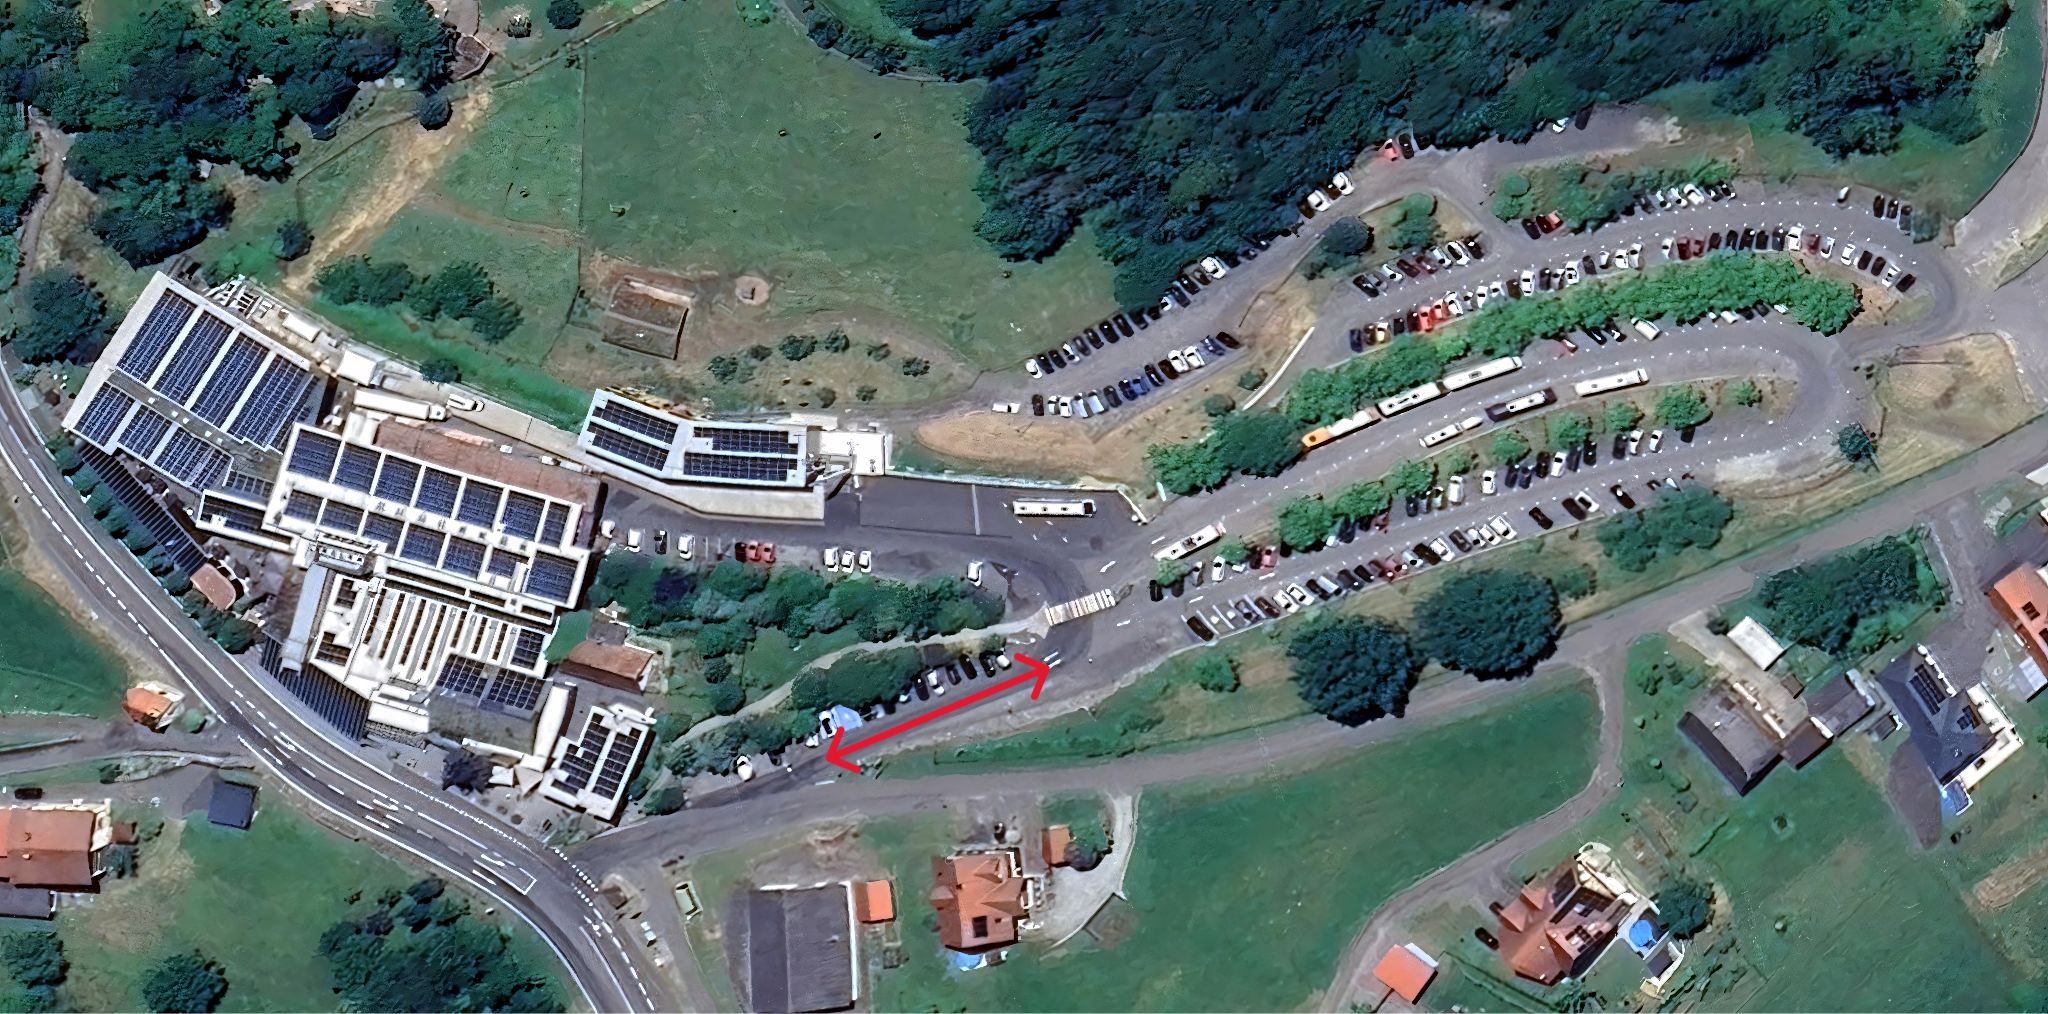
\includegraphics[width=\textwidth]{zotter.png}
    \caption{Luftbild des Hauptgebäudes und Parkplatz der Zotter Schokolade GmbH}
    \source{Google, Google Earth: \url{https://earth.google.com/}}
    \label{fig:zotter_luftbild}
\end{figure}

\newpage
\subsubsection{Anforderungsanalyse an die Hardware}

\paragraph{Grundanforderungen}
Wie oben kurz erwähnt, existieren einige Anforderungen, welche für die Funktionsfähigkeit des Systems unausweichlich sind.
Zunächst galt es, die Gegebenheiten vor Ort zu betrachten, also Lage und Aufbau des Bereiches, in dem der Fahrzeugverkehr erkannt werden sollte.

Wie das Luftbild (Abb. \ref{fig:zotter_luftbild}) zeigt, verfügt der Parkplatz über eine kombinierte Ein- und Ausfahrt.
Dies reduziert zwar den Installationsaufwand der Hardware, erhöht jedoch die Software-Komplexität, da die Bewegungsrichtung der Fahrzeuge softwareseitig erkannt werden muss.
Das Zeitintervall zwischen zwei aufeinanderfolgenden Fahrzeugen wurde aufgrund der Breite der Einfahrt auf zwei bis drei Sekunden geschätzt.
Das System sollte folglich in der Lage sein, 20 bis 30 Bilder pro Minute zu analysieren und die daraus gewonnenen Daten persistent zu speichern.

\paragraph{Anforderungen Kamera}
Da die Kamera im Außenbereich eingesetzt wird, ist eine gewisse Witterungsbeständigkeit zwingend erforderlich.
Aufgrund der notwendigen Positionierung der Kamera sollte diese mindestens die Schutzklasse IP66 (Ingress Protection) erfüllen,
was einem Schutz vor starken Wasserstrahlen aus allen Richtungen entspricht. \cite{baseus_ip_ratings}

Da das Kennzeichenerkennungssystem primär für die Erfassung von Kunden-Kennzeichen konzipiert ist, ist von einer effektiven Hauptbetriebszeit während der Öffnungszeiten der Zotter-Erlebniswelt ausgegangen worden.
Diese betragen: Mo--Fr: 9--18 Uhr, Sa: 9--18:30 Uhr.
Aufgrund dessen lag im Entscheidungsprozess kein großes Augenmerk auf den Nachtsichtfähigkeiten des Kamerasystems.

\paragraph{Anforderungen Server}
Die notwendige Rechenleistung des Servers hängt sehr stark von der Komplexität und Art der Prozesse ab, welche auf diesem ausgerollt und aktiv sind.
Deshalb wurde diese anfangs absichtlich nicht genau definiert.
Festgelegt wurde jedoch der Einsatz eines Linux-Betriebssystems, da dieses dem internen Unternehmensstandard entspricht, einen geringen OS-Overhead aufweist und eine breite Kompatibilität bietet.
Dies wurde allerdings als zweitrangig betrachtet, da das System durch die Verwendung von Containerisierung mit Docker ohnehin eine Plattformunabhängigkeit bietet.
Auch wurde seitens Zotter vorausgesetzt, dass sämtliche Daten nicht nur aus Datenschutzgründen On-Premise, sondern für eine bessere Isolation des Systems lokal auf dem eingesetzten Server gespeichert werden sollen.


\subsubsection{Evaluierung der Hardware-Optionen}

\paragraph{Kamera -- Auswahl}

In Bezug auf die Kamera wurden von Anfang an nur IP-Kameras in Betracht gezogen, also Kameras, bei denen Video-Streams und Kommunikation per Ethernet stattfinden.
Dies hat zwei Hauptgründe:
Daten können zunächst in den meisten Fällen direkt per API-Requests ausgelesen werden, entweder über HTTP/REST-APIs oder im Fall von Video-Streams über RTSP (Real Time Streaming Protocol).
Zudem nutzen viele IP-Kameras PoE (Power over Ethernet) für ihre Spannungsversorgung, was die Aufbaukomplexität weiter minimiert, da nur ein Kabel, welches Strom und Daten überträgt, verlegt werden muss. \cite{wiki_ip_camera}

Vor dem offiziellen Start der Diplomarbeit wurden hierzu schon einige Überlegungen angestellt und mögliche Produkt-Kandidaten vorgemerkt.
Im Zuge von Gesprächen mit Michael Zotter wurde darauf aufmerksam gemacht, dass bereits einige IP-Kameras des Herstellers Synology für frühere Testversuche angeschafft wurden.
Besonders das Modell BC500, von welchem einige Stück bereits im Besitz der Firma Zotter waren, erschien als besonders geeignet. \cite{synology_bc500}

\begin{figure}[htbp]
    \centering
    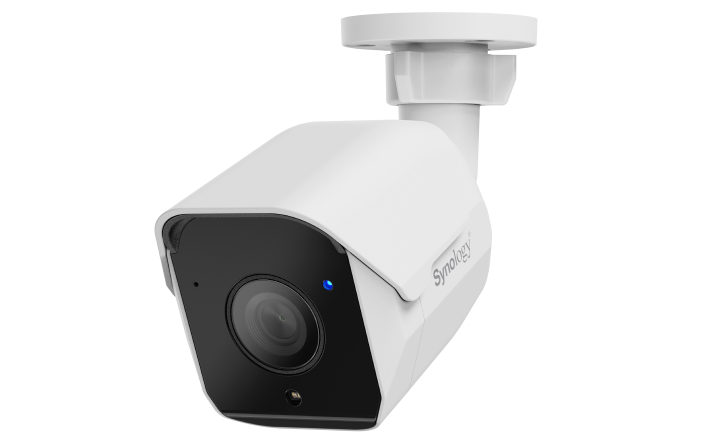
\includegraphics[width=8cm]{synology_bc500.png}
    \caption{Synology BC500}
    \source{\url{https://fileres.synology.com/images/ec/products/BC500.jpg}}
    \label{fig:synology_bc500}
\end{figure}

Mit einer Witterungsbeständigkeitsbewertung von IP67, da als Außenkamera konzipiert, ist diese gut für den Außeneinsatz geeignet.
Die maximale Videoauflösung von 2880$\times$1620 Pixel bei maximal 30 FPS erschien auch für eine konsistente Kennzeichenerkennung ausreichend.
Auch verfügt die BC500 über eine automatische Nachtsichtfunktion mittels Infrarot-LEDs.
Zusätzlich schien die BC500 über eine robuste API für das Auslesen von Daten und das Streamen des Feeds zu verfügen.

Aufgrund der oben angesprochenen sofortigen Verfügbarkeit und des wegfallenden Mehraufwands für diese Kamera, verbunden mit den genannten Spezifikationen, fiel die Entscheidung nach Absprache mit unserer Kontaktperson auf das Synology-Modell.

\newpage
\paragraph{Kamera -- Montage}

Das Kamerasystem wurde, wie unten erkenntlich (Abb. \ref{fig:kamera_montage}), so montiert, dass es in Richtung des Parkplatzes zeigt.
Dies erwies sich als die optimale Wahl, da so der mögliche Erkennungsbereich maximiert wird und die Montage an dieser Position einfacher realisierbar war.
Bei der genauen Positionierung und Ausrichtung der Kamera wurde versucht, sich so gut wie möglich am Kamera-Setup-Guide von Plate Recognizer zu orientieren. \cite{platerecognizer_camera_setup}

Die erforderliche Netzwerkverkabelung wurde, wie oben im Bild ersichtlich, über den bereits vorhandenen Kabelkanal der Sicherheitsschranke geführt.
Dieser verläuft bis in den Netzwerkschrank im angrenzenden Bürogebäude, wo die Anbindung an das Firmennetzwerk erfolgt.

\begin{figure}[htbp]
    \centering
    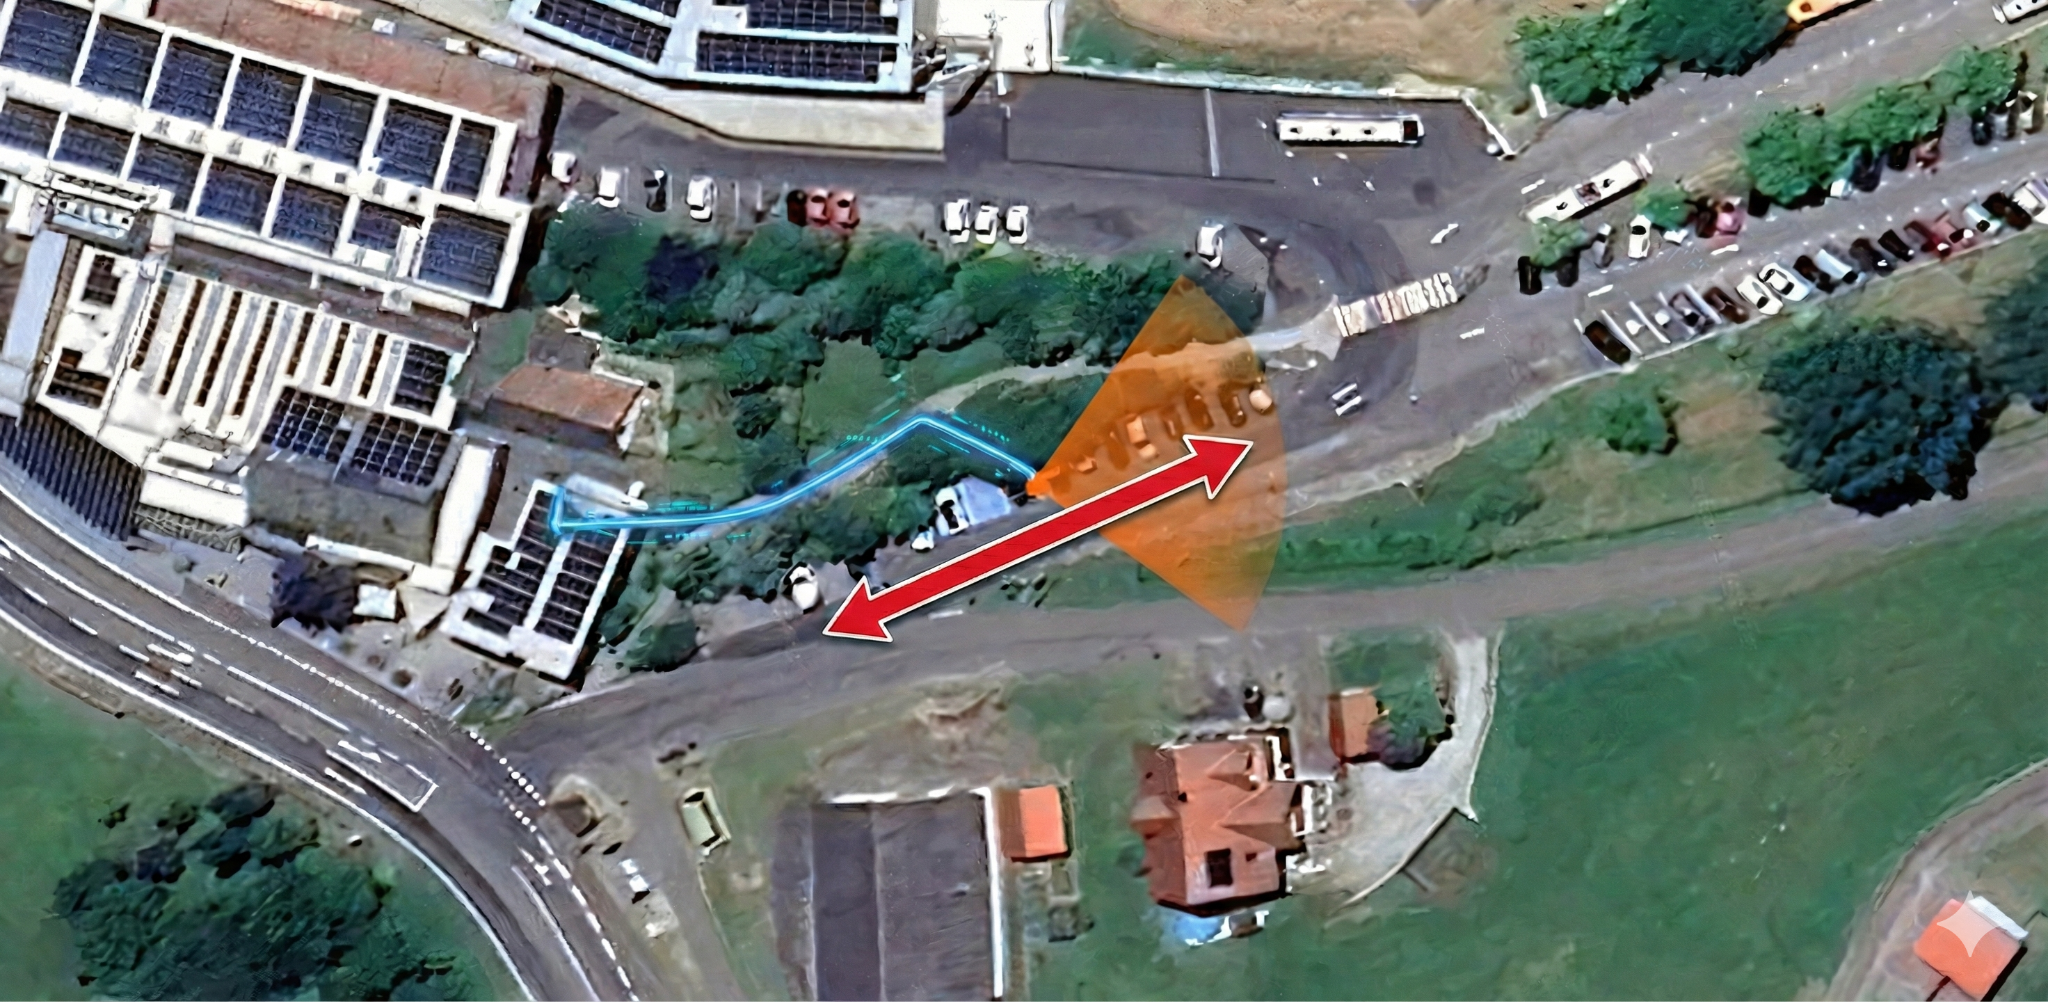
\includegraphics[width=\textwidth]{zotter-markup.png}
    \caption{Markup der Kamerapositionierung}
    \source{Google, Google Earth: \url{https://earth.google.com/}}
    \label{fig:kamera_montage}
\end{figure}

\newpage
\paragraph{Server -- Auswahl}

Die gewählte Microservice-Architektur im Zusammenspiel mit der angewandten Containerisierung erlaubt eine hohe Flexibilität für die Art der benötigten Hardware.
Des Weiteren war aus einem früheren Praktikum bei Zotter Schokolade bekannt, dass die hausinterne Infrastruktur Kapazitäten für Container-Deployment bietet.

Als zweite Option wurde das Einrichten eines kleinen Servers auf der Hardware eines Office-Mini-PCs erwogen.
Dieser wäre aus reiner Implementierungs- und Funktionssicht mit der ersten Option gleichwertig, mit dem Vorteil, dass dieser Ansatz eine gewisse Unabhängigkeit zum internen Netzwerk und zur zentralen Infrastruktur ermöglicht.

An diesem Punkt wurde im Kamera-Entscheidungsprozess auf die bestehenden Synology-Produkte aufmerksam gemacht.
Mit dieser Neuausrichtung kam die Idee auf, das System auf einem eigenen NAS-System (Network-attached Storage), ebenfalls von Synology zu betreiben.

Nicht nur wurden NAS-Systeme von Synology bereits im Unternehmen eingesetzt, diese sind in den meisten Bereichen gleichwertig mit den vorherigen beiden diskutierten Ansätzen und bieten in manchen Bereichen klare Vorteile \cite{aws_nas}:
\begin{enumerate}
    \item Die Vorteile der zweiten Option bleiben bestehen, es gibt weiterhin eine gesteigerte Unabhängigkeit zur Unternehmensinfrastruktur und damit hergehend mehr Entwicklungsfreiheit.
    \item Da es sich um ein NAS-System handelt, also ein Gerät, welches primär für die Speicherung von Daten konzipiert ist, stellt der benötigte Speicherplatz kein Problem mehr dar, da einfach neue Disks verbaut werden können (z.B. 2$\times$ 2TB Disks, RAID 1).
    \item Diese NAS-Systeme besitzen bereits leistungsstarke Komponenten, welche in Bezug auf Rechenleistung meist gleichwertig zu einem durchschnittlichen Mini-PC sind.
          Auch sind die meisten NAS-Geräte mit einem vollwertigen Betriebssystem ausgestattet, welches Methoden bereitstellt, um Container mittels Docker reibungslos laufen zu lassen.
\end{enumerate}

Der größte Vorteil kommt aber mit der Kombination mit den oben beschriebenen Kameras des gleichnamigen Herstellers.
Wie die Kameralinie von Synology vermuten lässt, bietet der Hersteller eigene Produkte gezielt für Überwachungsaufgaben an.
Diese laufen unter einem Gesamtsystem mit der Bezeichnung "`Surveillance Station"' und sind als Paket auf den hauseigenen NAS-Systemen verfügbar. \cite{synology_surveillance}

\newpage
Innerhalb des Surveillance Station-Ökosystems bietet Synology mit der DVA-Serie (Deep Video Analytics) spezialisierte NVR-Geräte (Network Video Recorder) an, welche über GPU-beschleunigte KI-Funktionen verfügen.
Insbesondere das Modell DVA1622 (zur Zeit des Projekts das einzige verfügbare Modell der DVA-Serie) bietet für diese Diplomarbeit in Kombination mit der Kamera BC500 viele Vorteile: \cite{synology_dva}

\begin{figure}[htbp]
    \centering
    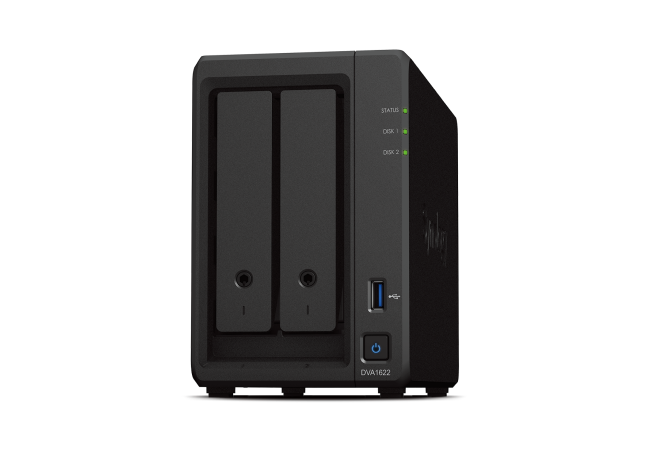
\includegraphics[width=8cm]{synology_dva1622.png}
    \caption{Synology DVA1622}
    \source{\url{https://www.synology.com/img/products/detail/DVA1622/heading.png}}
    \label{fig:synology_dva1622}
\end{figure}

Zunächst bietet die Surveillance Station API Zugriff auf Live-Streams, Snapshots und Ereignis-Metadaten, was die Integration in eigene Microservices im Vergleich zum direkten Auslesen aus Kameras erheblich vereinfacht.
Die DVA-Serie unterstützt nativ viele Features aus dem Security- und Surveillance-Bereich.
So können etwa mittels Erkennungszonen bereits auf Surveillance Station-Ebene relevante Bildbereiche wie der Einfahrtsbereich definiert werden. \cite{synology_dva}
Dies ist besonders für das Erstellen von "`Triggers"' relevant, also das Anlegen eines Bereiches, in dem im Falle einer Fahrzeugdurchfahrt die Kennzeichenerkennung stattfinden soll.
Des Weiteren können alle Kamera-Einstellungen, Aufzeichnungen und Analysen über eine einheitliche Oberfläche auf dem NAS-Gerät verwaltet werden. \cite{synology_surveillance}

Die Kombination aus relevanten Features, umfassender API und nativer Kamera-Unterstützung machte das Synology DVA1622-NAS zur optimalen Wahl für die Realisierung des Kennzeichenerkennungssystems.


\paragraph{Server -- Montage}

Das NAS-System ist durch seine Kompaktheit und Kapselung auf keine besonderen Anforderungen an den Montage- bzw. Betriebsort angewiesen.
Aus diesem Grund wurde dieses innerhalb des Bürogebäudes installiert, in welchem auch die Kamera an das Firmennetzwerk angeschlossen ist.

\newpage
\subsection{Technik-Stack und Technologieauswahl der Kennzeichenerkennung}
\label{sec:techstack}

\subsubsection{Technologieauswahl Kennzeichenerkennung}

Für die eigentliche Kennzeichenerkennung stand die Entscheidung zwischen der Entwicklung einer eigenen Lösung auf Basis von Open-Source-OCR-Bibliotheken (wie Tesseract OCR oder EasyOCR) und der Verwendung einer kommerziellen Lösung im Raum.

Bei der Evaluation von Tesseract und EasyOCR zeigte sich, dass diese generischen OCR-Engines zwar für Texterkennungsaufgaben gut geeignet sind, bei der spezifischen Herausforderung der Kennzeichenerkennung jedoch erhebliche Nachteile aufweisen.
Kennzeichen stellen besondere Anforderungen an ein Erkennungssystem, wie im Kapitel~\ref{sec:alpr} bereits erwähnt:
Sie müssen aus verschiedenen Winkeln, bei unterschiedlichen Lichtverhältnissen, mit Verschmutzungen und in Bewegung zuverlässig erkannt werden.
Zudem variieren Kennzeichenformate international stark in Schriftart, Layout und Zeichenabständen.

Als weitere Option wurde die Verwendung der Synology-nativen Lösung zur Kennzeichenerkennung erwogen.
Dies erwies sich aber schnell als nicht umsetzbar, da die Erkennung laut Hersteller auf dem Modell DVA1622 nur für stationäre Fahrzeuge ausgelegt ist. \cite{synology_lpr}

Die Entwicklung eines eigenen trainierten Modells auf Basis dieser Bibliotheken hätte einen erheblichen Aufwand für das Sammeln und Annotieren von Trainingsdaten bedeutet, wobei die resultierende Genauigkeit dennoch fraglich geblieben wäre.
In diese Richtung wurden im Zuge der Diplomarbeit-Entwicklung Prototypen erstellt, diese blieben aber in ihrer Qualität unzureichend oder waren in ihrem Realisierungsaufwand unrealistisch.

Aus diesem Grund fiel die Entscheidung auf Plate Recognizer, eine spezialisierte kommerzielle Lösung für Kennzeichenerkennung.
Plate Recognizer bietet hochoptimierte Machine-Learning-Modelle, welche bereits auf Kennzeichenbildern aus über 90 Ländern trainiert wurden. \cite{platerecognizer_countries}
Dies gewährleistet eine deutlich höhere Erkennungsrate auch unter erschwerten Bedingungen \cite{platerecognizer_results}.
Wie im Kapitel~\ref{sec:mmc} erwähnt bietet diese Lösung, zusätzlich zur reinen Texterkennung, erweiterte Funktionen wie Fahrzeugtyp- und Farberkennung, welche für zukünftige Erweiterungen des Systems nützlich sein können.

Ein weiterer entscheidender Vorteil ist die Verfügbarkeit als Docker-Container (Plate Recognizer SDK), der vollständig lokal auf dem DVA1622 NAS betrieben werden kann.
Im Gegensatz zu Cloud-basierten API-Lösungen bleiben damit alle Bilddaten im lokalen Netzwerk, was sowohl Datenschutzanforderungen erfüllt als auch Latenzzeiten minimiert. \cite{platerecognizer_snapshot}


\subsubsection{Argumentation der Software-Technologien Entscheidungen}

Als Web-Framework wurde FastAPI auf Python gewählt \cite{fastapi}, welches moderne asynchrone Request-Verarbeitung unterstützt und automatische API-Dokumentation via OpenAPI/Swagger generiert.
Im Vergleich zu Flask, dem vermutlich bekanntesten Python-Framework, bietet FastAPI native Type-Hints-Unterstützung und automatische Validierung von Request-/Response-Daten durch Pydantic. \cite{jetbrains_frameworks}
Gegenüber dem schwergewichtigeren Django bringt FastAPI deutlich weniger Overhead mit und ist damit besser für kleine Microservices geeignet, bei denen schlanke, spezialisierte Services bevorzugt werden. \cite{jetbrains_frameworks}

Für die Datenhaltung wurde PostgreSQL als relationale Datenbank gewählt. \cite{postgresql}
Während NoSQL-Datenbanken wie MongoDB für hochskalierbare, dokumentenbasierte Anwendungen Vorteile bieten, sprechen im vorliegenden Fall die strukturierten Datenbeziehungen (Erkennungen, Benutzer etc.) klar für eine relationale Datenbank.

Um Datenbank-Schema Änderungen versioniert und reproduzierbar zu gestalten, wurde Alembic als Migrations-Framework gewählt \cite{alembic}.
Im Gegensatz zu manuellen SQL-Skripten ermöglicht dies rückverfolgbare Datenbankänderungen, die automatisiert über alle Umgebungen ausgerollt werden können.

Das Gesamtsystem basiert auf Docker und einer Microservice-Architektur.
Wie zuvor detailliert erklärt, läuft jeder Dienst (Data Collection, Notification, Grafana) in seinem eigenen Container mit klar definierten Schnittstellen.
Dies verhindert wie in den Theoretischen Grundlagen erklärt nicht nur Abhängigkeitskonflikte zwischen verschiedenen Services, sondern ermöglicht auch die unabhängige Skalierung einzelner Komponenten.
Die Containerisierung gewährleistet zudem Plattformunabhängigkeit, da das System problemlos von der Synology-Plattform auf andere migriert werden kann, ohne dass Anpassungen am Code notwendig sind.

\newpage

% Kapitel 4: Systementwurf und Architektur
% Kapitel 4: Systementwurf und Architektur
\section{Systementwurf und Architektur}
\label{sec:systementwurf}

\subsection{Gesamtarchitektur}
\label{sec:gesamtarchitektur}

Das System wurde als hybride Microservice-Architektur konzipiert, in der jeder funktionale Bereich als eigenständiger, containerisierter Service realisiert wird.

Für den Entwurf der Systemarchitektur wurde die Design-Methodik der "`The 12-Factor App"' \cite{twelve_factor} herangezogen.
Diese definiert eine Reihe von Best-Practices für die Entwicklung moderner Applikationen.
Im Rahmen dieser Arbeit wurden insbesondere die strikte Trennung von Konfiguration und Code durch Umgebungsvariablen (Faktor III), die Behandlung der Datenbank als angebundener Backing-Service (Faktor IV) sowie die Sicherstellung der Parität zwischen Entwicklungs- und Betriebsumgebung durch Containerisierung und CI/CD (Faktor X) umgesetzt. Auf die genaue Umsetzung der Faktoren wird in den betreffenden Kapiteln genauer eingegangen.

Hybrid bedeutet in diesem Kontext primär, dass die einzelnen Services nicht ganzheitlich isoliert und entkoppelt sind, da nicht jeder dieser über eine eigene Datenhaltung verfügt.
Stattdessen nutzen alle Komponenten einen gemeinsamen PostgreSQL Service, welcher auf Schema-Ebene isoliert ist.
Auf dieses Konzept wird im Kapitel~\ref{sec:db_architektur} näher eingegangen.
Die Gesamtarchitektur wurde so entworfen, dass diese die in der Aufgabenstellung definierten Anforderungen abbildet.
Im Zuge der Entwicklung wurden nicht alle der im folgenden Kapitel erwähnten Komponenten implementiert, die bereits konzipierten Services werden dennoch in diesem Kapitel aus Gründen der Vollständigkeit erwähnt.

\begin{figure}[htbp]
    \centering
    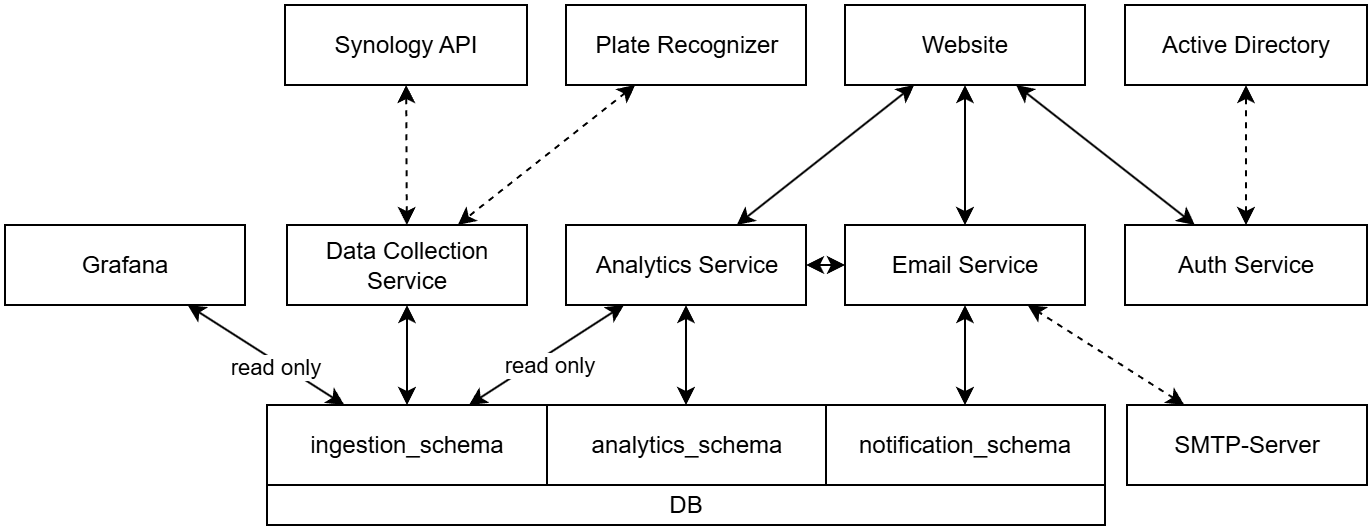
\includegraphics[width=\textwidth]{architektur.png}
    \caption{Architektur Diagramm}
    \label{fig:architektur}
\end{figure}

Wie in der Abbildung erkenntlich besteht diese Diplomarbeit aus Komponenten, welche sich in drei primäre Kategorien einteilen lassen: Backend-, Frontend- und Infrastruktur-Services.
Darüber hinaus bestehen Anbindungen an externe Services (wie etwa die Plate Recognizer SDK).
Sofern diese implementiert wurden, werden sie im Kapitel Implementierung (Abschnitt~\ref{sec:implementierung}) beim jeweiligen Dienst im Detail erläutert.
Die Architektur folgt bewusst keinem API-Gateway Ansatz, wie es oft bei Microservice-Ansätzen typisch ist, da die Services primär intern kommunizieren und nur wenige Endpunkte nach außen hin offen zugänglich sind.


\subsubsection{Backend-Services}

Das funktionale Backend des Systems bilden vier Python-Services basierend auf dem FastAPI-Framework.
Der Data Collection Service nimmt als Herzstück des Systems Webhook-Events der Synology Surveillance Station entgegen, sobald eine Fahrzeugbewegung im definierten Erkennungsbereich erkannt wurde.
Dieser beantragt daraufhin einen Kamera-Snapshot, leitet diesen an die Plate Recognizer SDK weiter und speichert die verarbeiteten, anonymisierten Ergebnisse in der Datenbank.

Der Notification Service hat Möglichkeiten, um Benutzer-Einstellungen bezüglich E-Mail-Benachrichtigungen zu verwalten und den Versand dieser via SMTP zu steuern.
Dieser Service kann etwa benutzt werden, um Tagesstatistiken oder Ähnliches mit Hilfe des Analytics Service bereitzustellen.

Der eben erwähnte Analytics Service (Auswertungsservice) wurde konzipiert, um analytische Endpunkte bereitzustellen, über welche Auswertungen und Vorhersagen aus gesammelten Erkennungsdaten abgerufen werden können.

Der Auth Service soll laut Konzeption Benutzer der Web-Oberfläche gegen das unternehmensinterne Active Directory authentifizieren, um eine nahtlose Integration in die bestehende Unternehmensinfrastruktur zu ermöglichen.


\subsubsection{Frontend}

Als Benutzeroberfläche sollte primär der Web Service, eine mit Next.js \cite{nextjs} realisierte Web-Applikation dienen.
Diese wurde als zentrale Oberfläche für Konfiguration und Verwaltung von Benachrichtigungen konzipiert und kommuniziert ausschließlich über REST-APIs mit den Backend-Services.
Als Übergangslösung und zweite Visualisierungsplatform dient Grafana, in Form eines Dashboards für diverse Statistiken.


\subsubsection{Infrastruktur-Services}

Die Infrastruktur-Ebene umfasst mehrere Stützkomponenten, die den Betrieb des Gesamtsystems ermöglichen.
PostgreSQL fungiert als zentrale relationale Datenbank für die persistente Datenhaltung aller Services.
Der Plate Recognizer SDK-Container stellt das lokal betriebene ALPR-Modell als REST-API bereit, sodass die Bildverarbeitung vollständig im lokalen Netzwerk stattfindet wie zuvor im Kapitel~\ref{sec:on_premise} bereits ausführlich erklärt wurde.
Ein DB-Prestart-Container übernimmt die automatische Initialisierung der Datenbank beim Systemstart.
Ergänzend sorgt ein Backup-Container für regelmäßige, automatisierte Datenbanksicherungen.
Die Details zu diesen Infrastruktur-Komponenten werden im Kapitel~\ref{sec:infrastruktur} näher erläutert.


\subsubsection{Kommunikationswege}
\label{sec:kommunikationswege}

Die Kommunikation zwischen den Services erfolgt ausschließlich über RESTful HTTP-APIs.
Der primäre Kommunikationsweg im System, welcher für die Datenerfassung erfolgt, lässt sich wie folgt zusammenfassen:

\paragraph{1. Externer Trigger durch Erkennung eines Fahrzeugs $\to$ Data Collection Service}

\begin{figure}[htbp]
    \centering
    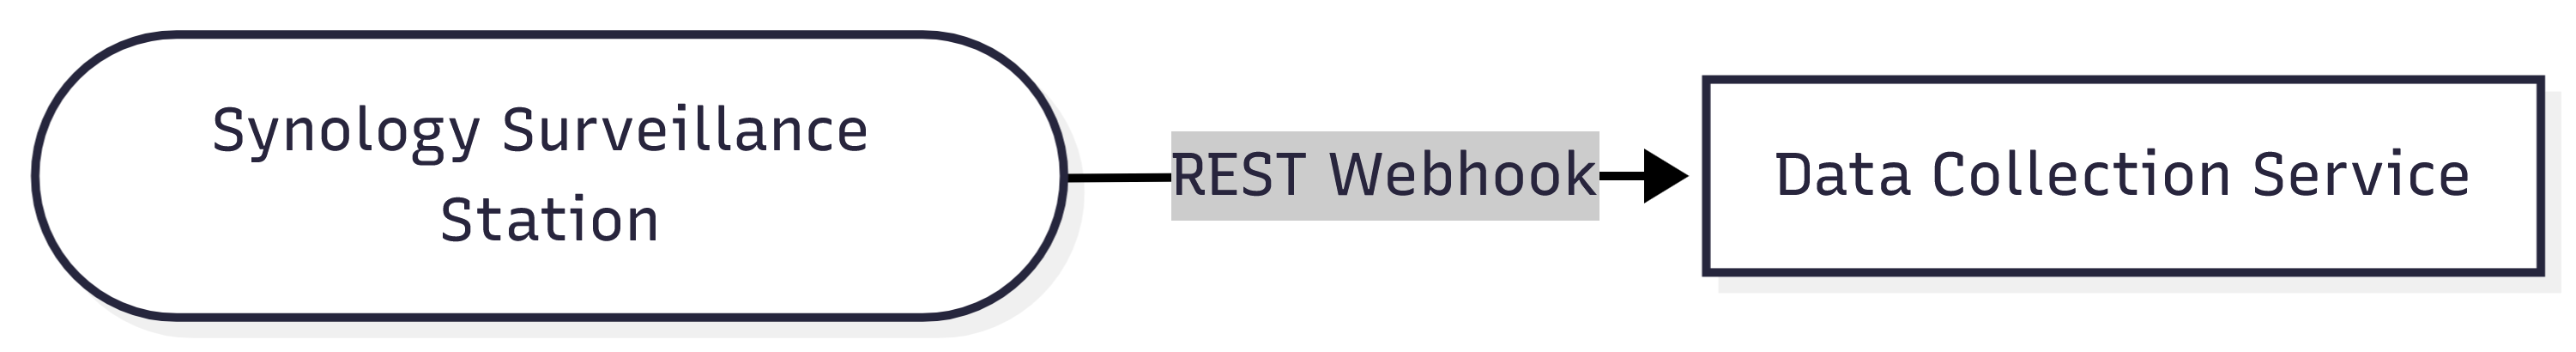
\includegraphics[width=0.8\textwidth]{trigger_for_data_collection.png}
    \caption{Trigger für den Data Collection Service}
    \label{fig:trigger}
\end{figure}

Die Synology Surveillance Station ruft bei Erkennung einer Fahrzeugbewegung einen REST-Webhook des Data Collection Service auf.

\paragraph{2. Data Collection Service $\to$ Synology API}

\begin{figure}[htbp]
    \centering
    
\includegraphics[width=0.8\textwidth]{data_collection_to_synology.png}
    \caption{Data Collection Service zu Synology API}
    \label{fig:dc_to_synology}
\end{figure}

Nach Empfang des Webhooks authentifiziert sich der Service bei der Synology-API, um einen aktuellen Kamera-Snapshot abzurufen.

\paragraph{3. Data Collection Service $\to$ Plate Recognizer SDK}

\begin{figure}[htbp]
    \centering
    
\includegraphics[width=0.8\textwidth]{data_collection_to_plate_recognizer.png}
    \caption{Data Collection Service zu Plate Recognizer SDK}
    \label{fig:dc_to_pr}
\end{figure}

Der abgerufene Snapshot wird als Bilddatei per HTTP an den lokal betriebenen Plate Recognizer Container gesendet, der die Kennzeichenerkennung durchführt und das Ergebnis als JSON zurückgibt.

\paragraph{4. Data Collection Service $\to$ PostgreSQL}

\begin{figure}[htbp]
    \centering
    
\includegraphics[width=0.8\textwidth]{data_collection_to_db.png}
    \caption{Data Collection Service zu DB}
    \label{fig:dc_to_db}
\end{figure}

Die verarbeiteten und anonymisierten Erkennungsergebnisse werden direkt in die Datenbank geschrieben.

\vspace{0.5cm}
Weitere konzipierte, teils implementierte Verbindungen:

\paragraph{5. Web Service $\to$ Backend-Services}

\begin{figure}[htbp]
    \centering
    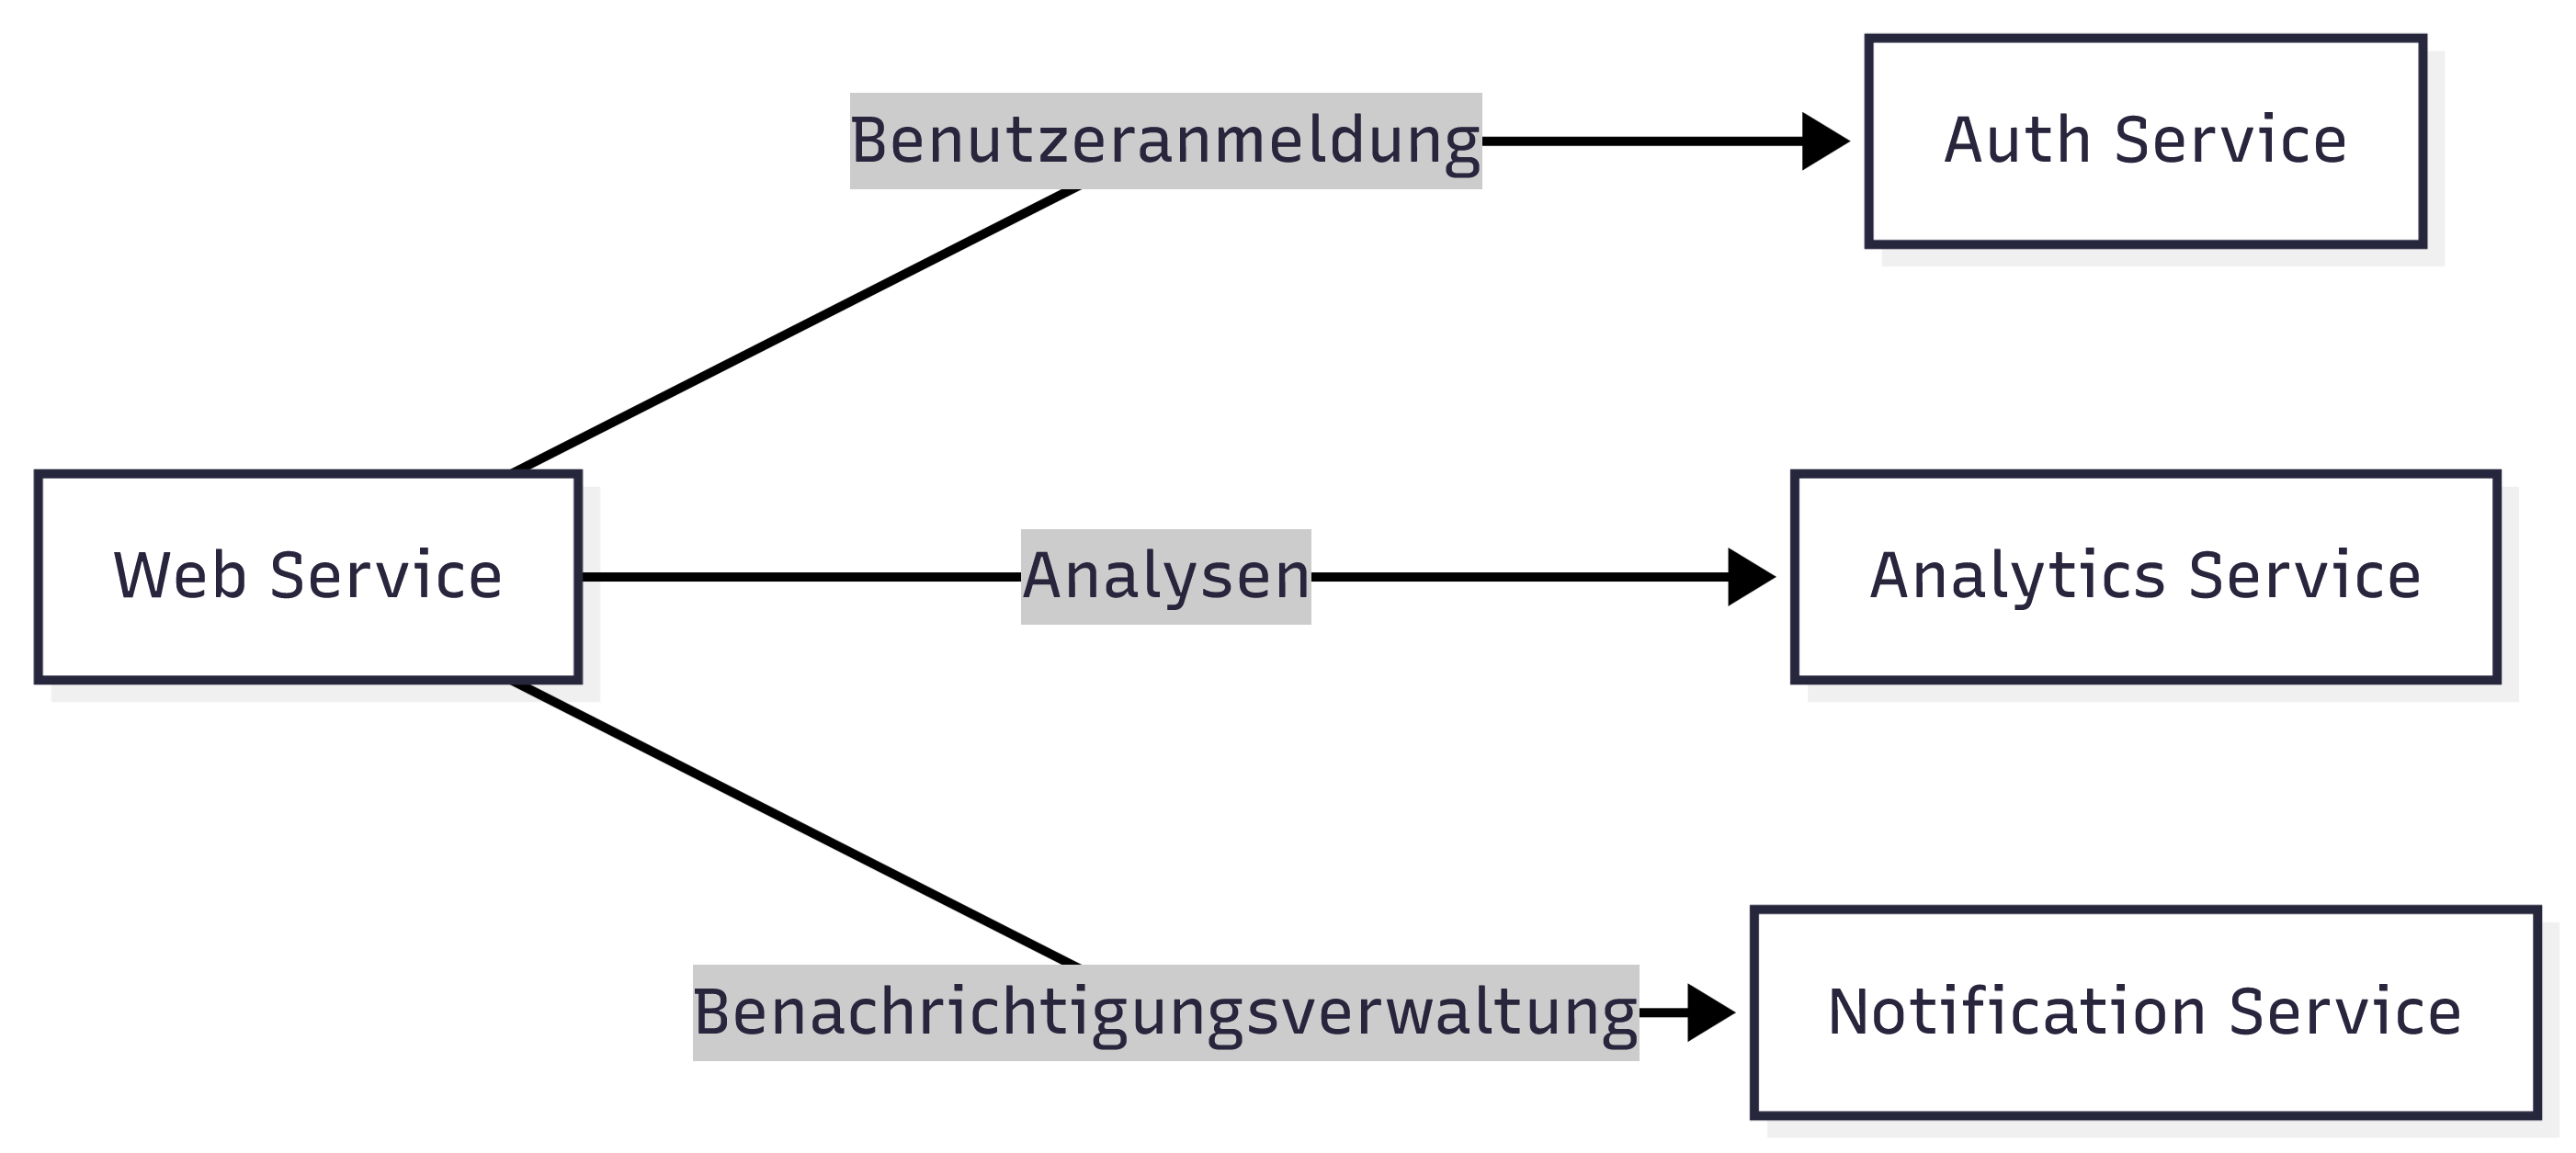
\includegraphics[width=0.8\textwidth]{web_interactions.png}
    \caption{Web Service Interaktionen}
    \label{fig:web_interactions}
\end{figure}

Die Web-Oberfläche kommuniziert über REST-Calls mit dem Auth Service (Benutzeranmeldung), dem Analytics Service für Analysen und dem Notification Service (Benachrichtigungsverwaltung).

\paragraph{6. Notification Service $\to$ Analytics Service}

\begin{figure}[htbp]
    \centering
    
\includegraphics[width=0.8\textwidth]{notification_to_analytics.png}
    \caption{Notification Service zu Analytics Service}
    \label{fig:notif_to_analytics}
\end{figure}

Für den Versand von periodischen Zusammenfassungen ruft der Notification Service Daten vom Analytics Service ab.

\paragraph{7. Grafana $\to$ PostgreSQL}

\begin{figure}[htbp]
    \centering
    
\includegraphics[width=0.8\textwidth]{grafana_to_db.png}
    \caption{Grafana zu DB}
    \label{fig:grafana_to_db}
\end{figure}

Grafana greift über einen Read-only Datenbankbenutzer lesend auf das Data-Collection-Schema der Datenbank zu, um das Dashboard mit aktuellen Daten zu versorgen.


\subsection{Datenbankdesign}
\label{sec:datenbankdesign}

\subsubsection{Architekturansatz}
\label{sec:db_architektur}

Anstatt für jeden Microservice eine eigene PostgreSQL-Instanz zu betreiben, wurde eine Single-Database-Strategie auf Basis einer PostgreSQL-Instanz mit Schema-basierter Isolation gewählt \cite{postgresql_schemas}.
Innerhalb der gemeinsam genutzten PostgreSQL-Datenbank existieren also drei, logisch getrennte Schemas:

\begin{enumerate}
    \item Das Data-Collection-Schema (Ingestion) enthält die Kerndaten der Fahrzeugerkennungen.
    \item Das Analytics-Schema (Analytics) ist für aggregierte oder vorberechnete Analysedaten konzipiert.
    \item Das Notification-Schema (Notification) speichert Nutzerpräferenzen für den Benachrichtigungsdienst.
\end{enumerate}

Dieser Ansatz, eine einzelne Datenbankinstanz durch Schemas logisch zu unterteilen, anstatt mehrere Instanzen zu betreiben, bietet im Kontext dieser Diplomarbeit mehrere Vorteile:
Zunächst reduziert er den operativen Aufwand, da nur eine Datenbankinstanz verwaltet, gesichert und überwacht werden muss, wie es etwa bei einer klassischen Microservice-Architektur der Fall wäre.
Dennoch bleibt die logische Trennung der Daten gewährleistet, da jeder Service nur auf sein zugewiesenes Schema zugreifen kann.
Des Weiteren vereinfacht er Cross-Schema-Lesezugriffe, etwa kann der Analytics Service oder Grafana Abfragen direkt auf die Ingestion-Daten zugreifen, ohne dass dafür eine Datenreplikation oder zusätzliche API-Aufrufe zwischen Services nötig sind.
Die Zugriffskontrolle wird dabei über dedizierte PostgreSQL-Benutzer mit minimalen Berechtigungen erzwungen, was im Abschnitt zum Sicherheitskonzept näher beleuchtet wird.


\subsubsection{Entitäten und ER-Modell}

Das Datenbankschema des Systems umfasst zwei zentrale Entitäten, welche sich in getrennten Schemas befinden.

Die Tabelle \texttt{vehicle\_observations} im Data-Collection-Schema ist die zentrale Entität des gesamten Systems.
Jeder Datensatz repräsentiert eine einzelne erfasste Fahrzeugerkennung und bildet die Grundlage für sämtliche Analysen und Visualisierungen.
Die Tabelle speichert neben dem Erkennungszeitpunkt und einem anonymisierten Hash des Kennzeichens auch den Konfidenzwert der Erkennung, das Herkunftsland, gegebenenfalls den Bezirk (für österreichische und slowenische Kennzeichen), Fahrzeugkategorie, Marke, Modell, Farbe sowie die Fahrtrichtung.
Letztere wird durch die Orientierung des Fahrzeugs (Vorder- oder Rückseite sichtbar) ermittelt und ermöglicht damit die Unterscheidung zwischen Ein- und Ausfahrten.

Die Tabelle \texttt{user\_preferences} im Notification-Schema verwaltet die Benachrichtigungseinstellungen der Systembenutzer.
Sie speichert pro Benutzer den Namen und E-Mail Adresse sowie zwei Flags, welche festlegen, ob der Benutzer Echtzeit-Alerts oder periodische Zusammenfassungen per E-Mail erhalten möchte.

Die folgende Darstellung zeigt die Attribute der beiden Entitäten als ER-Diagramm:

\begin{figure}[htbp]
    \centering
    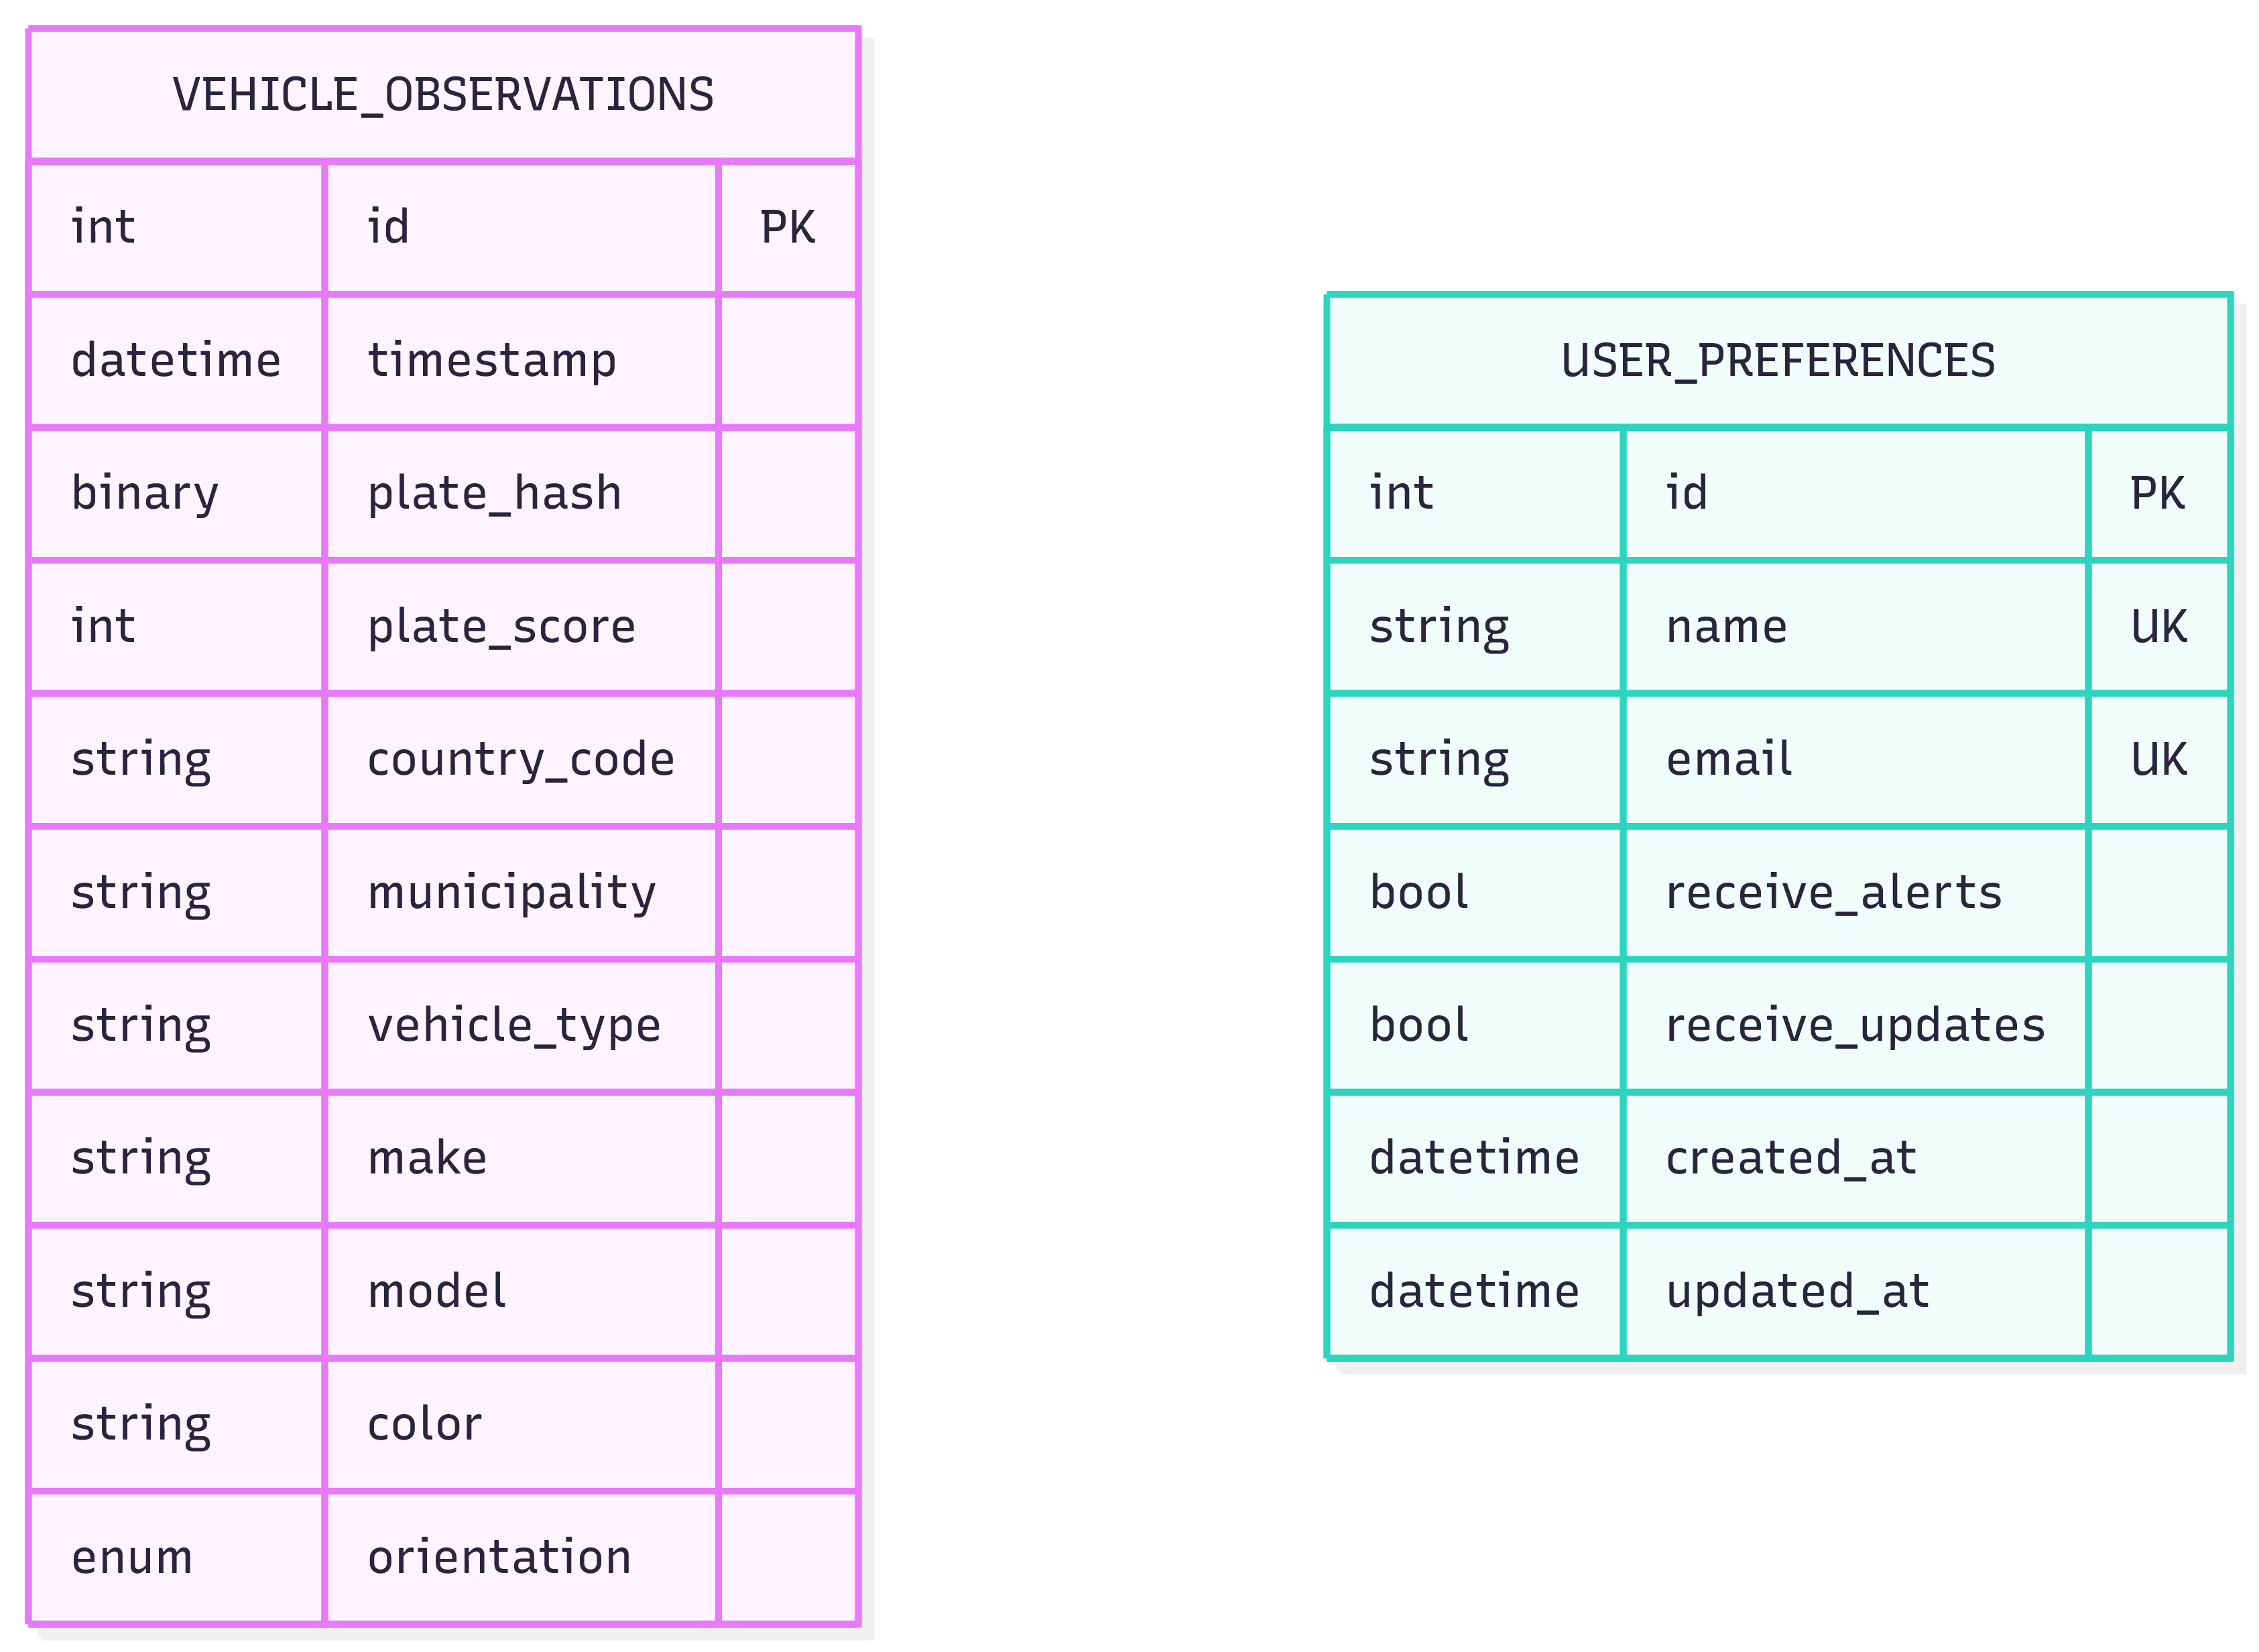
\includegraphics[width=0.8\textwidth]{tables.png}
    \caption{Datenbank Tabellen}
    \label{fig:db_tables}
\end{figure}


\subsubsection{Argumentation zur Denormalisierung}
\label{sec:denormalisierung}

Das Datenbankschema der \texttt{vehicle\_observations} Tabelle ist bewusst nicht vollständig normalisiert.
Statt etwa \texttt{country\_code}, \texttt{vehicle\_type}, \texttt{make}, \texttt{model} und \texttt{color} in eigene Lookup-Tabellen mit Foreign-Key-Relationen auszulagern, werden diese direkt als Strings in der Observationstabelle gespeichert.

Diese Entscheidung beruht auf mehreren Gründen:

\paragraph{1. Datenherkunft aus externer API}
Die Daten werden direkt aus der JSON-Antwort der Plate-Recognizer-API übernommen.
Die API gibt eine flache Struktur zurück, in welcher das Erkennungsresultat alle Attribute bereits als einfache Zeichenketten oder Werte enthält.
Das Erstellen und die Wartung eines normalisierten Schemas mit Lookup-Tabellen für dynamische, von einer externen API stammende Werte, würde unnötige Komplexität hinzufügen und einen laufenden Wartungsaufwand bedeuten, da neue Werte (z.B. neue Fahrzeugmodelle) oder etwa Benennungsanpassungen kontinuierlich eingepflegt werden müssten.

\paragraph{2. Lesedominanz}
Die Daten werden primär lesend konsumiert, sowohl von Grafana für Dashboard-Visualisierungen als auch vom konzipierten Analytics-Service.
Bei leselastigen Workloads sind Verknüpfungen über mehrere Tabellen teurer als direkte Abfragen auf einer einzelnen, denormalisierten Tabelle.

\paragraph{3. Einfachheit der Abfragen}
Die Grafana-Dashboards verwenden direkte SQL-Abfragen. Eine einfache, flache Tabellenstruktur macht diese Abfragen nicht nur lesbarer, sondern eliminiert auch die Fehleranfälligkeit, die durch komplexe JOIN-Befehle entstehen könnte.

\paragraph{4. Unveränderlichkeit der Daten}
Fahrzeugerkennungen sind unveränderliche Ereignisse, im Gegensatz zu beispielsweise einem Produktkatalog, wo sich der Name eines Herstellers ändern kann, sind gespeicherte Erkennungen statisch.
Die Hauptvorteile einer Normalisierung, etwa die konsistente Aktualisierung gemeinsamer Daten, sind daher nicht wirklich relevant.

\paragraph{5. Speicherplatz als unkritische Ressource}
Die durch die Denormalisierung entstehende Datenredundanz, etwa wiederholt gespeicherte Herstellernamen, führt zu einem geringfügig höheren Speicherbedarf.
Dieser ist im vorliegenden Anwendungsfall jedoch vernachlässigbar, da das System auf einer NAS-Plattform mit erweiterbarem Speicher betrieben wird und die Datensatzgröße pro Erkennung minimal ist.
Zum Stand der Dokumentation dieser Arbeit beträgt ein volles Backup der gesamten Datenbank (Über 60.000 Erkennungen) ca. 3.4 MB.
Um diesen Punkt zu verdeutlichen, wurde die theoretische Dauer bis zur vollständigen Kapazitätsauslastung des verbauten NAS-Systems ermittelt.

\paragraph{Formel zur Berechnung der Speicherauffüllungsdauer anhand der Größe eines Full-Backups:}

\begin{equation}
    \label{eq:speicher}
    T = \frac{S_{\max} \cdot D_t}{G_t}
\end{equation}

wobei $T$ Tagen der Dauer bis zum vollständigen Befüllen eines Speicherplatzes $S_{\max}$ in Bytes entspricht, $G_t$ die Größe eines Full-Backups in Bytes und $D_t$ die vergangenen Tage seit Beginn der Kennzeichenerfassungen zum Zeitpunkt $t$ darstellen.

Als verfügbarer Speicherplatz $S_{\max}$ wurde 1TB ($10^{12}$ Bytes) angenommen, da dies dem halben, derzeit im NAS-System verbauten Speicher entspricht.
$G_t$ betrug (Stand 12. Februar 2026) wie bereits oben erwähnt rund 3,4MB ($3{,}4 \cdot 10^{6}$ Bytes) und zu diesem Stand sind 188 Tage ($D_t$) seit Beginn der Aufzeichnungen vergangen.

Es gilt dementsprechend:

\begin{equation}
    T = \frac{10^{12} \cdot 188}{3{,}4 \cdot 10^6} \approx 5{,}53 \cdot 10^{7} \text{ Tage} / 365{,}25 \approx 151387 \text{ Jahre}
\end{equation}

Das 1TB-NAS würde daraus folgend bei gleichbleibendem Wachstum also erst in rund 151 Tausend Jahren voll sein.
Die Speicherkapazität ist damit für den praktischen Betrieb als unbegrenzt zu betrachten, selbst wenn der verfügbare Speicher als erheblich kleiner angenommen wird.

\footnote{Es ist anzumerken, dass die Größe eines Full-Backups zwar in einem linearen Zusammenhang mit der tatsächlichen Datenbankgröße steht, diese aber zum Beispiel durch Komprimierung nicht vollständig widerspiegelt \cite{so_backup_size, sqlskills_backup}.
    Auch nehmen die Erkennungs-Einträge nicht den gesamten Platz des Backups ein, da andere Daten wie etwa die anderer Services ebenfalls in diesem enthalten sind.
    Das oben genannte Ergebnis ist aus diesen Gründen nur als Annäherung zu betrachten, wobei die Kernaussage ohne Zweifel bestehen bleibt.}

Die Herleitung dieser Formel ist dem Anhang zu entnehmen.


\subsection{Sicherheitskonzept}
\label{sec:sicherheitskonzept}

Die Sicherheitsarchitektur des Systems ist in mehrere Schichten gegliedert, die jeweils unterschiedliche Aspekte des Schutzes adressieren.


\subsubsection{Authentifizierung und Endpunkt-Sicherheit}

Die Absicherung der API-Endpunkte erfolgt je nach Service und Anforderung durch unterschiedliche Mechanismen:

\paragraph{Data Collection Service (HTTP Basic Authentication)}
\label{sec:dc_auth}
Der Webhook-Endpunkt \texttt{/api/vehicle\_detected}, über den die Synology Surveillance Station Fahrzeugerkennungen meldet, ist durch HTTP Basic Authentication geschützt.
Die Zugangsdaten werden dabei gegen die Synology-Credentials des Systems validiert.
HTTP Basic Authentication ist dabei die einzige von der Surveillance Station unterstützte Authentifizierungsmethode für Webhook-Aufrufe, weshalb hier keine Alternative in Frage kam.
Da der Endpunkt ausschließlich für die maschinenbasierte Kommunikation innerhalb des lokalen Netzwerks vorgesehen ist und nicht von außen erreichbar ist, ist dieses Sicherheitsniveau für diesen Anwendungsfall ausreichend.

\paragraph{Notification Service (API-Key Authentication)}
\label{sec:notif_auth}
Der Notification Service erwartet einen statischen API-Key im Authorization-Header jeder Anfrage.
Die Entscheidung gegen eine komplexere Authentifizierung, etwa mittels JWT (JSON Web Tokens) oder Session-basierter Tokens fiel aus mehreren Gründen:
Erstens findet die Kommunikation mit dem Notification Service ausschließlich intern zwischen Services statt, nicht direkt durch Endbenutzer,
zweitens würde eine JWT-basierte Lösung eine Schlüsselverwaltung (Signing Keys, Token-Rotation, Expiration-Handling) erfordern, die für einen reinen Service-zu-Service-Call unnötige Komplexität hinzufügt.
Die Notwendigkeit eines statischen API-Key, der über Umgebungsvariablen konfiguriert wird, kommt daher, dass der Port dieses Services zu Testzwecken freigeschaltet wurde.
Für diesen Zweck bietet ein Token ein angemessenes Sicherheitsniveau bei geringer Komplexität.

\paragraph{Auth Service / Web Service (Active Directory Integration)}
Für die Authentifizierung von Benutzern der Web-Oberfläche wurde die Integration mit dem bestehenden Active Directory (AD) der Firma Zotter konzipiert.
Dieser sollte mittels LDAP (Lightweight Directory Access Protocol)-Anbindung Nutzerdaten aus dem firmeninternen Microsoft-AD Server beziehen und diese für den Login-Prozess nutzen.
Dies bietet den Vorteil, dass keine separate Benutzerverwaltung implementiert und gewartet werden muss und die bestehende Unternehmensinfrastruktur zur Zugangskontrolle genutzt werden kann.


\subsubsection{Datenbankzugriffskontrolle}
\label{sec:db_zugriff}

Ein zentrales Element der Sicherheitsarchitektur ist die konsequente Anwendung des Principle of Least Privilege, kurz PoLP auf Datenbankebene \cite{wiki_polp}.
Jeder Service operiert mit einem eigenen, dedizierten PostgreSQL-Benutzer, dessen Rechte auf das absolut notwendige Minimum beschränkt sind.

Durch diese Segmentierung wird sichergestellt, dass im Falle einer Infiltration eines einzelnen Services der Zugriff auf Daten anderer Bereiche verhindert wird.
Der Notification Service kann beispielsweise keine Fahrzeugerkennungsdaten auslesen, und ein Angreifer mit Zugriff auf den Analytics Service könnte keine Daten verändern, da er nur Leserechte auf das Ingestion-Schema besitzt.

Die folgende Darstellung visualisiert die Berechtigungsstruktur:

\begin{figure}[htbp]
    \centering
    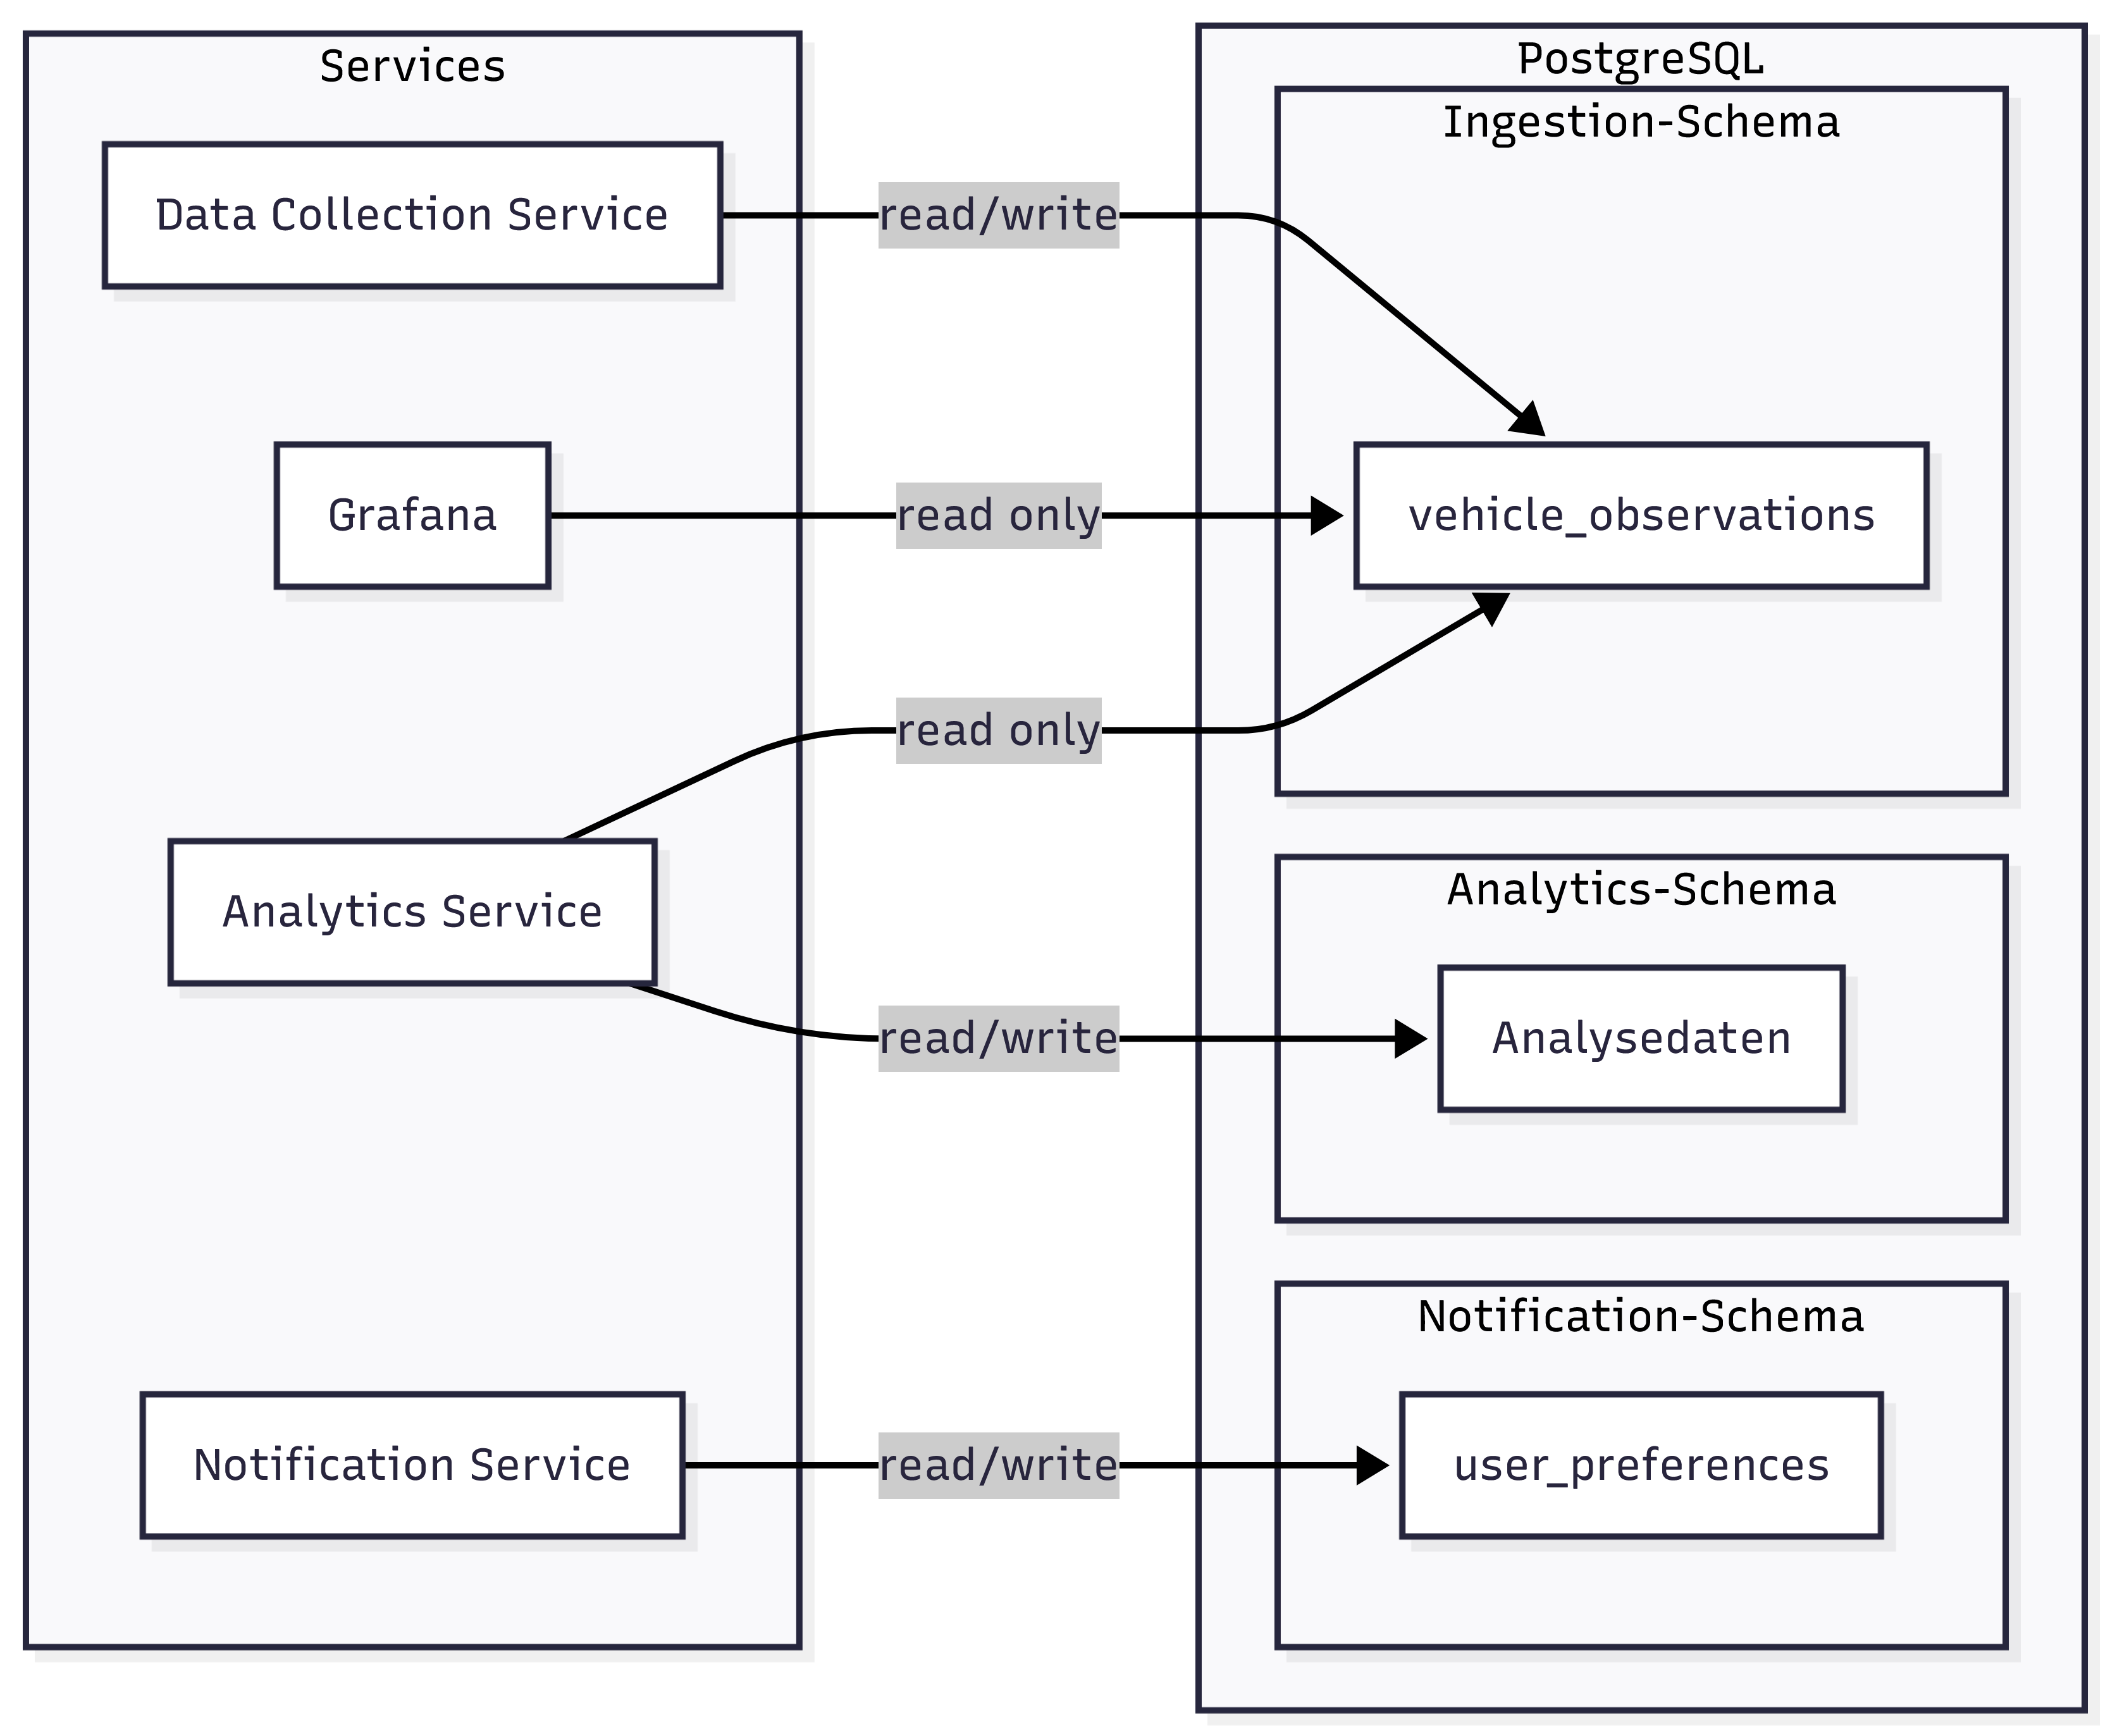
\includegraphics[width=0.8\textwidth]{db_user.png}
    \caption{DB Benutzer}
    \label{fig:db_user}
\end{figure}

Wie die Darstellung zeigt, hat der Data-Collection-User Vollzugriff auf das Ingestion-Schema, der Analytics-User nur Lesezugriff darauf (aber Vollzugriff auf das eigene Analytics-Schema), und der Notification-User ist vollständig auf das Notification-Schema beschränkt.
Grafana greift über den \texttt{analytics\_user} ebenfalls ausschließlich lesend auf die Ingestion-Daten zu.


\subsubsection{Datenschutz und Umgang mit Kennzeichen-Daten}
\label{sec:datenschutz}

Der Umgang mit Kennzeichen-Daten ist aus DSGVO-Perspektive besonders sensibel, da Kennzeichen als personenbezogene Daten klassifiziert werden \cite{dsgvo_personenbezogen}.
Das System implementiert deswegen eine mehrstufige Anonymisierungsstrategie:

\paragraph{1. Irreversibles Hashing}
Unmittelbar nach der Erkennung wird das Kennzeichen mittels SHA-256 gehasht.
Dieser Hash ist ein kryptographisch sicherer, irreversibler Einwegprozess.
Heißt, aus dem gespeicherten Hash kann das Originalkennzeichen nicht mehr rekonstruiert werden, zwei erkannte Kennzeichen können dennoch auf ihre Gleichheit analysiert werden.
In der Datenbank wird ausschließlich der 32-Byte-Hash (\texttt{plate\_hash}) gespeichert, nicht das Klartext-Kennzeichen.

\paragraph{2. Keine Speicherung von Bilddaten}
Die Kamera-Snapshots, aus welchen die Kennzeichen extraktiert werden, werden nicht persistent gespeichert.
Die Bilddaten existieren lediglich temporär im Arbeitsspeicher, während sie zur Erkennung verarbeitet werden.

\paragraph{3. Verarbeitung im lokalen Netzwerk}
Wie im Kapitel zur ALPR-Technologie erläutert, läuft der Plate Recognizer als lokaler Container.
Sämtliche Bilddaten und Erkennungsergebnisse verlassen zu keinem Zeitpunkt das lokale Netzwerk der Firma Zotter.


\subsubsection{Datenlebenszyklus (Data Lifecycle)}
\label{sec:data_lifecycle}

Der Lebenszyklus der Fahrzeugerkennung beschreibt den logischen Weg der Daten von der Erfassung bis zur langfristigen Sicherung.
Das Konzept ist so gestaltet, dass personenbezogene Daten so früh wie möglich eliminiert werden und nur anonymisierte, für die Analyse relevante Informationen persistent gespeichert werden.

\begin{figure}[htbp]
    \centering
    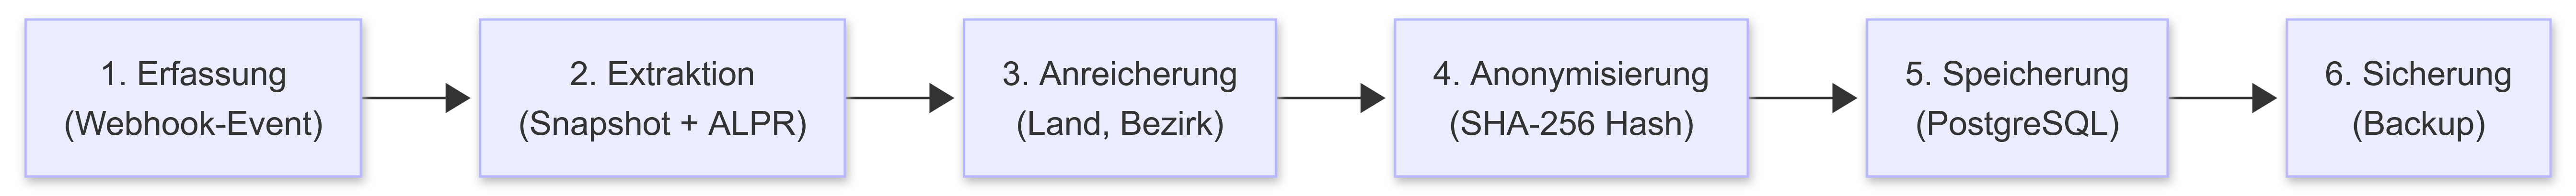
\includegraphics[width=\textwidth]{detection_flow.png}
    \caption{Detection Flow}
    \label{fig:detection_flow}
\end{figure}

Eine Fahrzeugbewegung im Erkennungsbereich löst ein Event aus (Erfassung), woraufhin ein Kamera-Snapshot angefordert und an die ALPR-Komponente gesendet wird (Extraktion), hierbei werden die Bilddaten nicht persistent gespeichert.
Die Erkennungsergebnisse werden anschließend, falls möglich, um regionale Herkunft auf Bezirksebene angereichert.
Darauf folgt die Anonymisierung, wobei das erkannte Kennzeichen mittels SHA-256 irreversibel gehasht wird.
Ab diesem Punkt existiert das originale Kennzeichen in keinem Teil des Systems mehr.
Der anonymisierte Datensatz wird in der PostgreSQL-Datenbank gespeichert und regelmäßig automatisiert gesichert (Details im Kapitel~\ref{sec:infrastruktur}).

Durch diesen Lebenszyklus ist sichergestellt, dass personenbezogene Daten zu keinem Zeitpunkt persistent gespeichert werden und die gespeicherten, anonymisierten Daten eine Rückverfolgung auf individuelle Fahrzeuge nicht ermöglichen.
Die konkrete technische Umsetzung der einzelnen Phasen wird im Kapitel~\ref{sec:implementierung} genauer beschrieben.

\newpage

% Kapitel 5: Implementierung
% Kapitel 5: Implementierung
\section{Implementierung}
\label{sec:implementierung}

Dieses Kapitel dokumentiert die technische Umsetzung der in der Architektur beschriebenen Komponenten.
Zunächst wird auf die Konfiguration der Synology Surveillance Station eingegangen, welche für einen korrekten Betrieb des Systems notwendig ist.
Für jeden Service werden die zentralen Abläufe, Designentscheidungen und relevante Code-Auszüge dargestellt, wobei der Fokus dieses Kapitels auf der Kernkomponente, dem Data Collection Service liegt.


\subsection{Konfiguration Synology Surveillance Station}

Auf der Surveillance-Station-Plattform können alle Bereiche des Synology Überwachungssystems konfiguriert werden.
Für diese Diplomarbeit sind jene Bereiche relevant, welche sich mit der Konfiguration der IP-Kameras, der Fahrzeugerkennung und der Aktionen (Trigger) befassen.


\subsubsection{IP Camera Konfiguration}

Mit dem IP Camera-Tool können Synology-Kameras im Netzwerk automatisch erkannt und konfiguriert werden.
In den Einstellungen der hinzugefügten IP-Kamera wurden Optionen wie die Bildrate oder Auflösung der Kamera maximiert, um die bestmöglichen Grundvoraussetzungen für eine erfolgreiche Erkennung zu bieten.

\begin{figure}[htbp]
    \centering
    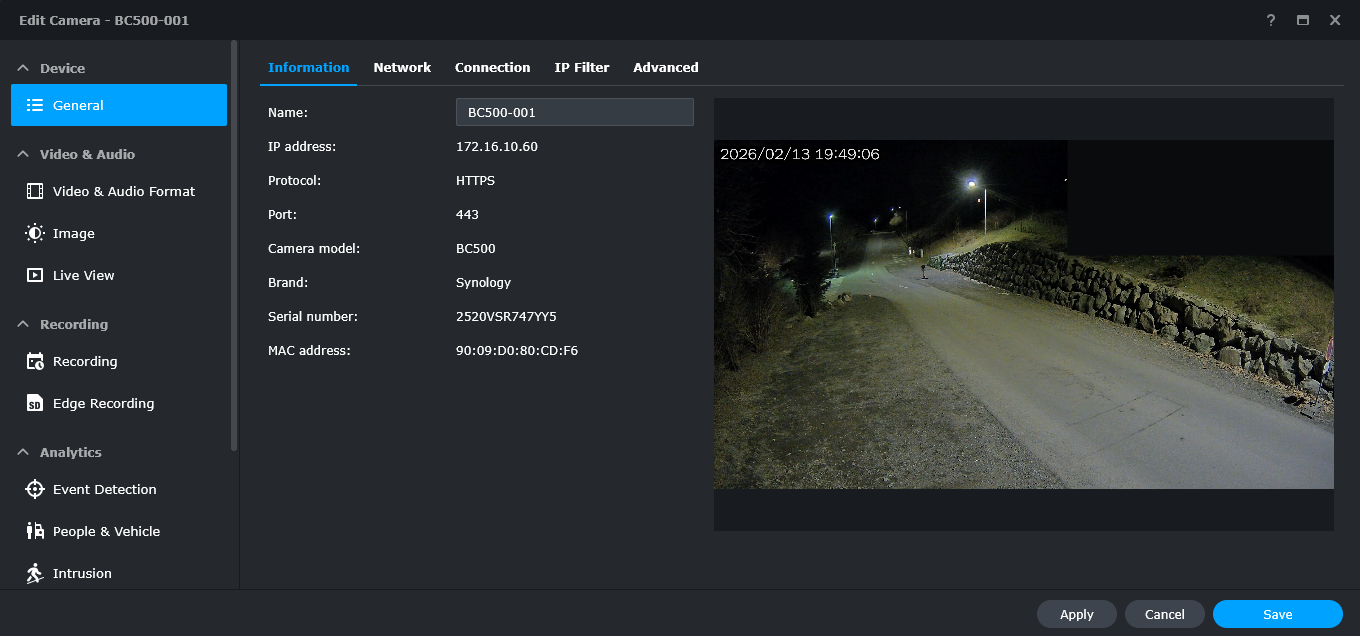
\includegraphics[width=\textwidth]{ip_camera_tool.png}
    \caption{IP Camera Tool}
    \label{fig:ip_camera_tool}
\end{figure}

\newpage
\subsubsection{Deep Video Analytics Konfiguration}

Da wie bereits im Kapitel~\ref{sec:hardware} erwähnt die Synology DVA-Serie als NAS-System gewählt wurde, standen für die Umsetzung dieses Projekts die erweiterten KI-Funktionen dieser Reihe zur Verfügung, diese werden von Synology als Deep Video Analytics (DVA) bezeichnet.
Eine dieser Funktionalitäten ist eine präzise und schnelle Durchfahrtskontrolle mittels Erkennungsbereichen.
Diese wurde genutzt, um den unten in der Abbildung erkenntlichen Bereich zu markieren, in welchem ein Trigger ausgelöst wird, sobald ein Fahrzeug diesen durchfährt.
Hierbei ist wichtig zu erwähnen, dass dieser DVA-Task so konfiguriert wurde, dass Fußgänger und stehende Fahrzeuge nicht erkannt werden.
Diese Einschränkungen sind wichtig, um das ALPR-System zu entlasten und Mehrfacherkennungen durch im Bereich befindliche, stationäre Fahrzeuge zu eliminieren.

\begin{figure}[htbp]
    \centering
    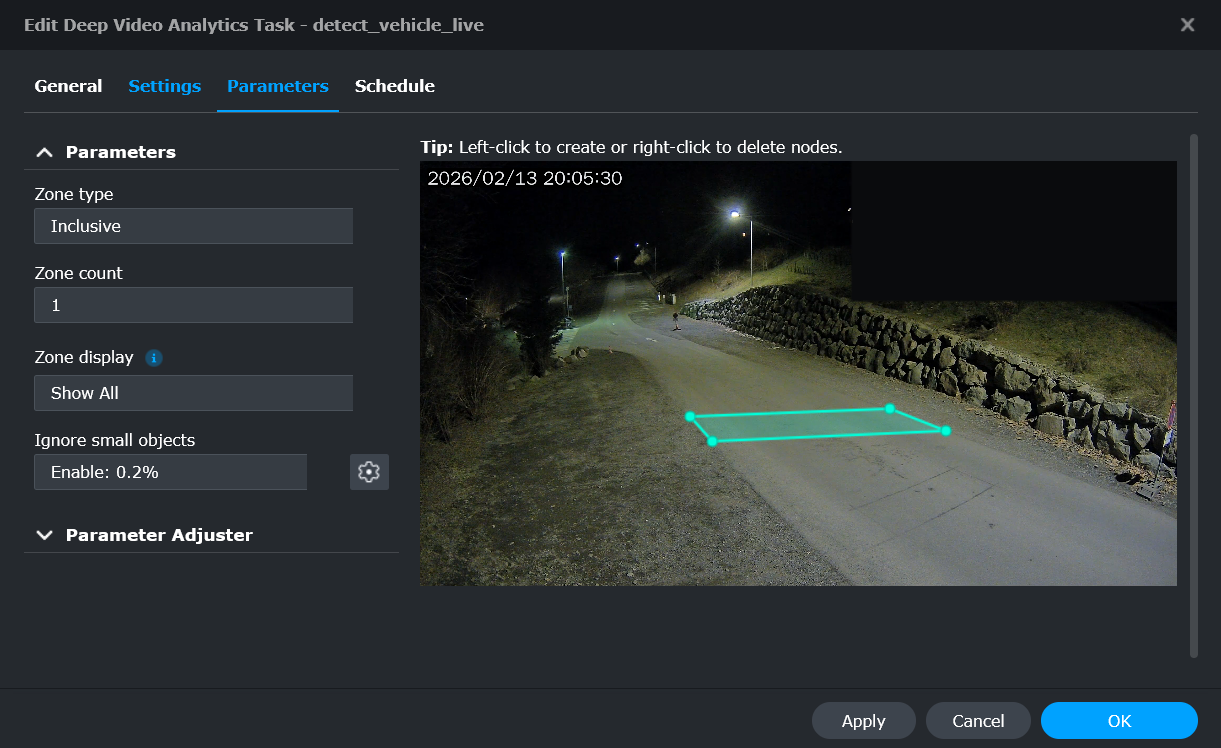
\includegraphics[width=\textwidth]{erkennungsbereich_config.png}
    \caption{Erkennungsbereich im Deep Video Analytics Tool\protect\footnotemark}
    \label{fig:erkennungsbereich}
\end{figure}
\footnotetext{Der in der Abbildung ersichtliche schwarze Balken in der rechten, oberen Ecke dient dem Datenschutz der auf der anderen Straßenseite befindlichen Familienhäuser und schränkt die Funktion des Systems in keiner Weise ein.}

\newpage
\subsubsection{Action Rule Konfiguration}

Innerhalb der Surveillance Station können sogenannte Action-Rules definiert werden, welche bei Erkennung einer Fahrzeugbewegung im konfigurierten Erkennungsbereich eine zuvor definierte Aktion ausführen.
Dieses System wird genutzt, um im Falle einer Erkennung dem Data Collection Service zu signalisieren, dass eine Fahrzeugerkennung stattgefunden hat.
Diese Aktionsregel wird aufgerufen, nachdem der zuvor konfigurierte DVA-Task ein Fahrzeug erkennt und ist damit der Startpunkt, für die im Backend stattfindende Verarbeitung der Bilddaten.
Wie in Abbildung~\ref{fig:action_rule} erkenntlich, ruft diese einen Webhook des Data Collection Service auf; dieser wird im Abschnitt~\ref{sec:externer_trigger} näher beleuchtet.

\begin{figure}[htbp]
    \centering
    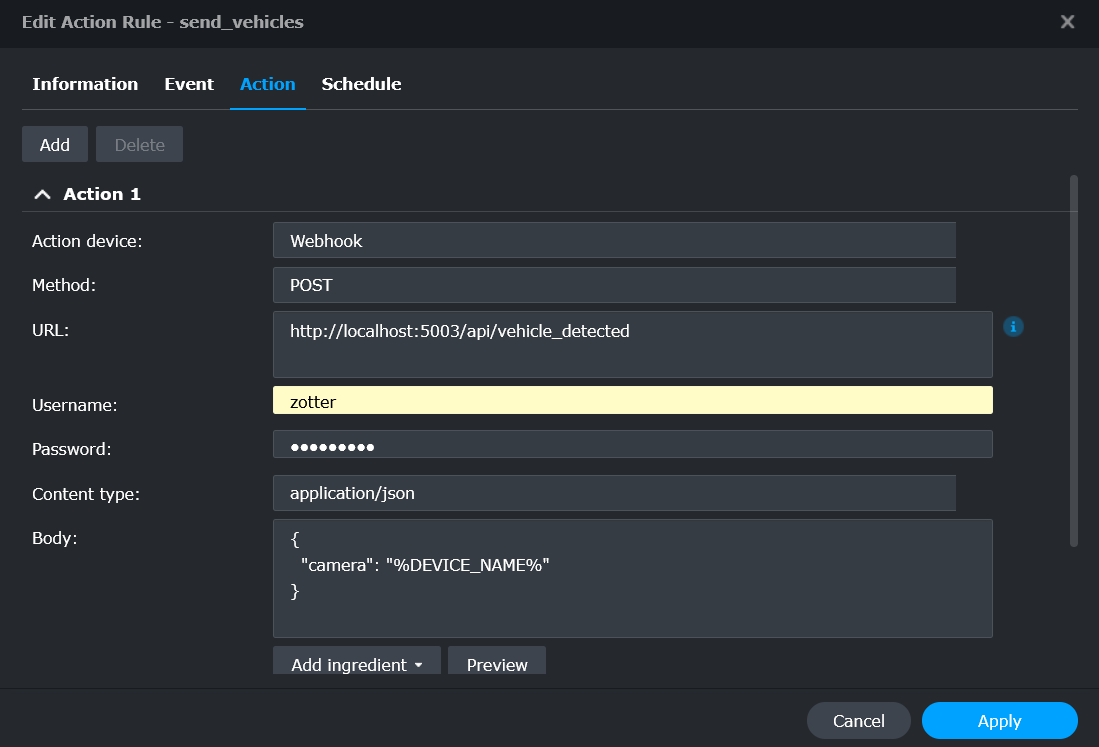
\includegraphics[width=\textwidth]{action_rule.png}
    \caption{Action-Rule für die Erkennung von Fahrzeugen}
    \label{fig:action_rule}
\end{figure}

\newpage
\subsection{Data Collection Service}

Der Data Collection Service bildet das funktionale Herzstück des gesamten Systems.
Dieser ist für die Entgegennahme von Fahrzeugerkennungsereignissen, die Beschaffung von Kamera-Snapshots, die Weiterleitung an die ALPR-Komponente zur Erkennung, sowie die Verarbeitung, Anonymisierung und persistente Speicherung der Ergebnisse verantwortlich.


\subsubsection{Konzept und Aufbau}

Der Service ist als FastAPI-Applikation implementiert und folgt einer modularen Architektur, wobei jeder funktionale Bereich in eigene Klassen, einen sogenannten Handler, ausgelagert ist, was eine klare Trennung der Verantwortlichkeiten (Separation of Concerns) ermöglicht:

\begin{itemize}
    \item \textbf{CameraHandler:} Dieser kapselt die gesamte Kommunikation mit der Synology Surveillance Station API (Authentifizierung, Kamera-Verwaltung, Snapshot-Abruf).
    \item \textbf{PlateRecognizerHandler:} Verwaltet die HTTP-Kommunikation mit dem Plate Recognizer SDK-Container.
    \item \textbf{CountryHandler:} Übernimmt die Anreicherung der Erkennungsdaten um regionale Herkunftsinformationen (Bezirkserkennung).
    \item \textbf{DatabaseHandler:} Verantwortlich für die Datenaufbereitung, Anonymisierung und die Speicherung der Erkennungen in der Datenbank.
\end{itemize}

Die Konfiguration des Services erfolgt über Umgebungsvariablen, welche mittels Pydantic Settings validiert werden \cite{pydantic_settings}.
Hierzu zählen unter anderem die Zugangsdaten für die Synology-API, der API-Key für Plate Recognizer, die Datenbankverbindungsparameter sowie ein konfigurierbares Duplikat-Erkennungsintervall.


\subsubsection{Externer Trigger}
\label{sec:externer_trigger}

Eine HTTP-Webhook ist wie zuvor erwähnt der Auslöser für die Verarbeitung der Bilddaten, welche von der Synology Surveillance Station bei der Erkennung eines Fahrzeugs aufgerufen wird. \cite{synology_webhooks}

Der Webhook-Endpunkt \texttt{POST /api/vehicle\_detected} erwartet im Request-Body den Namen der auslösenden Kamera und ist durch HTTP Basic Authentication geschützt, wie im Sicherheitskonzept (Abschnitt~\ref{sec:dc_auth}) erläutert.
Bei eingehenden Requests wird zunächst die Authentifizierung gegen die konfigurierten Synology-Credentials geprüft.
Nach erfolgreicher Validierung wird die Verarbeitung als Hintergrundaufgabe (Background Task) gestartet, während der Endpunkt sofort mit dem HTTP-Statuscode \texttt{202 Accepted} antwortet.

Dieses asynchrone Muster ist essenziell, um die Reaktionsfähigkeit des Systems zu gewährleisten und Blockaden während der Bildverarbeitung zu vermeiden.
Da die vollständige Verarbeitungskette, bestehend aus Snapshot-Abruf, ALPR-Analyse und Datenbankspeicherung, mehrere Sekunden in Anspruch nehmen kann, würde eine synchrone Verarbeitung die Surveillance Station blocken und potenzielle Folge-Events verzögern.
Durch die Entkopplung mittels Background Tasks wird sichergestellt, dass der Webhook-Endpunkt jederzeit mit minimaler Latenz erreichbar bleibt, und auch bei hoher Fahrzeugfrequenz keine Events aufgrund von Timeouts von der Surveillance Station verworfen werden.

Der Detektionszeitpunkt wird dabei bereits im HTTP-Endpoint erfasst und nicht erst im Background Task.
Dies stellt sicher, dass der Zeitstempel den tatsächlichen Zeitpunkt des Webhook-Aufrufs widerspiegelt und nicht den Zeitpunkt der eventuell verzögerten Verarbeitung.

\begin{lstlisting}[language=Python, caption={Webhook-Endpunkt für Fahrzeugerkennung}, label={lst:webhook}]
@app.post('/api/vehicle_detected')
async def handle_vehicle_detection(
    request: VehicleDetectionRequest,
    background_tasks: BackgroundTasks,
    credentials: HTTPBasicCredentials = Depends(basic_auth),
):
    if credentials.username != settings.synology_username \
       or credentials.password != settings.synology_password:
        raise HTTPException(status_code=401,
                            detail='Incorrect username or password')

    logger.info(f'Vehicle detected from camera: {request.camera}')

    detection_time = datetime.now()
    timestamp_str = detection_time.strftime('%Y%m%d_%H%M%S')

    background_tasks.add_task(
        process_vehicle_detection,
        request.camera,
        detection_time,
    )

    return {'status': 'accepted', 'timestamp': timestamp_str}
\end{lstlisting}


\newpage
\subsubsection{Ablauf der Verarbeitung}

Die im Anhang angeführte Darstellung (Abb. \ref{fig:data_collection_flow}) zeigt den vollständigen Ablauf von der Webhook-Auslösung bis zur Speicherung in der Datenbank als Sequenzdiagramm.
Jede Erkennung durchläuft nach dem Webhook-Eingang die folgenden Phasen, welche in den nächsten Unterkapiteln im Detail erläutert werden:
Kamera-Anbindung, ALPR-Aufruf, Datenanreicherung, Anonymisierung und Speicherung mit Duplikatprüfung.

\subsubsection{Kamera-Anbindung (CameraHandler)}

Die Kommunikation mit der Synology Surveillance Station erfolgt über die dezidierte Web-API dieser und ist in der CameraHandler-Klasse gekapselt \cite{synology_api}.
Der Ablauf der Kamera-Interaktion gliedert sich in drei Schritte:

\paragraph{1. Authentifizierung}
Zunächst authentifiziert sich der Service über den API-Endpunkt \texttt{SYNO.API.Auth} und erhält eine Session-ID (SID), die für alle nachfolgenden API-Aufrufe als Identifikation dient.

\paragraph{2. Kameraliste und Identifikation}
Im zweiten Schritt wird die Liste aller im Surveillance-Station-Netzwerk registrierten Kameras über den \texttt{SYNO.SurveillanceStation.Camera}-Endpunkt abgerufen.
Aus dieser Liste wird die Kamera anhand des vom Webhook übermittelten Namens identifiziert und die zugehörige Kamera-ID extrahiert.

\paragraph{3. Snapshot-Abruf}
Mit der ermittelten Kamera-ID wird über die \texttt{GetSnapshot}-Methode der Synology-API ein aktueller Kamera-Snapshot, also das Kamerabild zum Zeitpunkt der Anfrage, im JPEG-Format angefordert.
Die Bilddaten werden als Byte-Stream im Arbeitsspeicher gehalten, ohne auf die Festplatte geschrieben zu werden, um personenbezogene Bilddaten nicht persistent zu speichern.
Optional kann im Debug-Modus, welcher über eine Umgebungsvariable aktiviert wird, das Bild zu Diagnosezwecken auf die Festplatte geschrieben werden.

Jeder der drei Schritte ist durch spezifische Exceptions (\texttt{AuthenticationError}, \texttt{CameraDataError}, \texttt{SnapshotError}) abgesichert, die im Fehlerfall die Verarbeitungskette kontrolliert abbrechen.


\subsubsection{Plate Recognizer Integration (PlateRecognizerHandler)}

Die Bilddaten des Kamera-Snapshots werden, zur Kennzeichenerkennung, an den lokal betriebenen Plate Recognizer SDK-Container gesendet.
Die \texttt{PlateRecognizerHandler}-Klasse implementiert diesen HTTP-Aufruf mit einer Retry-Strategie mittels der tenacity-Bibliothek \cite{tenacity}:

\begin{lstlisting}[language=Python, caption={Plate Recognizer Integration mit Retry-Strategie}, label={lst:plate_recognizer}]
class PlateRecognizerHandler:
    @retry(
        wait=wait_fixed(1),
        stop=stop_after_attempt(5),
        retry=retry_if_exception_type(requests.HTTPError),
        reraise=True,
    )
    def send_to_api(self, api_key: str, image_data: bytes, 
                    camera_name: str, service_url: str) -> Any:
        image_buffer = BytesIO(image_data)
        response = requests.post(
            f'{service_url}/v1/plate-reader/',
            data={
                'camera_id': camera_name,
                'regions': ['at', 'hu', 'si', 'de'],
                'mmc': 'true',
                'direction': 'true',
            },
            files={'upload': image_buffer},
            headers={'Authorization': f'Token {api_key}'},
            timeout=15,
        )
        response.raise_for_status()
        return response.json()
\end{lstlisting}

Der \texttt{@retry}-Dekorator sorgt dafür, dass bei HTTP-Fehlern (etwa bei temporären Überlastungen oder Blockaden des ALPR-Containers) bis zu fünf Wiederholungsversuche im Abstand von einer Sekunde unternommen werden.
Dies erhöht die Robustheit des Systems, da kurzzeitige Ausfälle der ALPR-Komponente nicht zum Verlust von Erkennungen führen.

Der Parameter \texttt{regions} schränkt die Erkennung auf die relevanten Regionen ein, für diese Diplomarbeit wurden aufgrund der Lage der Zotter Schokolade GmbH, Österreich, Ungarn, Slowenien und Deutschland gewählt.
Dies verbessert die Erkennungsgenauigkeit, da das Modell die länderspezifischen Kennzeichenformate dieser Regionen priorisiert \cite{platerecognizer_api}.
Über den Parameter \texttt{mmc} (Make, Model, Color) wird die erweiterte Fahrzeugerkennung aktiviert, durch \texttt{direction} wird die Fahrtrichtung anhand der Fahrzeugorientierung angefordert.
Die Bilddaten werden als \texttt{BytesIO}-Objekt übergeben (ein im Arbeitsspeicher gehaltener Byte-Stream).


\subsubsection{Datenverarbeitung und Enrichment-Schleife}

Nach dem Empfang der JSON-Antwort von Plate Recognizer durchlaufen die Erkennungsdaten einen mehrstufigen Verarbeitungs- und Anreicherungsprozess, bis diese final und persistent in der Datenbank gespeichert werden.
Die Plate-Recognizer-API kann in einem einzelnen Bild mehrere Kennzeichen erkennen, weshalb die Antwort eine Liste von Ergebnissen enthält, welche jeweils einzeln in einer Schleife verarbeitet werden.

\paragraph{Datenextraktion}
Im ersten Schritt werden die relevanten Felder aus der Antwort der Plate-Recognizer-API extrahiert und in ein Pydantic-Schema überführt.
Die API liefert den Konfidenzwert jeder Erkennung als Float-Zahl zwischen 0 und 1 zurück, welcher für die Speicherung mit 1000 multipliziert und als ganzzahliger Wert abgelegt wird.
Die Fahrzeugorientierung wird aus der API-Antwort als Enum (\texttt{FRONT} oder \texttt{REAR}) abgebildet, wobei \texttt{FRONT} einer Ausfahrt und \texttt{REAR} einer Einfahrt entspricht, da die Kamera in Richtung des Parkplatzes filmt.

\paragraph{Bezirkserkennung (CountryHandler)}
Die Bezirkserkennung ist ein zentraler Bestandteil der Datenanreicherung und ermöglicht es, das Herkunftsbundesland bzw. den Herkunftsbezirk eines Fahrzeugs aus dem Kennzeichen abzuleiten.
Die Implementierung nutzt hierfür eine JSON-Datei (\texttt{municipalities.json}), welche Bezirkskürzel für österreichische \cite{oesterreich_kfz} und slowenische \cite{wiki_slovenia_plates} Kennzeichen deren vollen Namen und Bundesländern zuordnet.
Diese Zuordnungstabellen werden beim Start des Services einmalig in den Arbeitsspeicher geladen und als Dictionary-Lookup verwendet.

Der Erkennungsalgorithmus für österreichische Kennzeichen versucht zunächst, die ersten zwei Zeichen des Kennzeichens als Bezirkskürzel zu interpretieren.
Da einige österreichische Bezirke einbuchstabige Kürzel verwenden (wie z.B. "`W"' für Wien oder "`G"' für Graz), wird bei fehlgeschlagenem Zwei-Buchstaben-Lookup ein Fallback auf einbuchstabige Kürzel durchgeführt.

Für slowenische Kennzeichen wird ein ähnlicher Ansatz verfolgt, mit dem zusätzlichen Aspekt, dass der \texttt{CountryHandler} hier auch als Korrekturmechanismus dient:
Wird ein Kennzeichen von Plate Recognizer mit dem Ländercode \texttt{unknown} klassifiziert, der Kennzeichen-Präfix aber als slowenischer Bezirkscode erkannt, wird der Ländercode automatisch auf \texttt{si} korrigiert.
Diese Korrektur adressiert eine Limitierung der ALPR-Engine bei slowenischen Kennzeichen, welche aufgrund visueller Ähnlichkeiten zu anderen Formaten oft unerkannt bleiben.

\paragraph{Anonymisierung (Hashing)}
Nach der Datenanreicherung folgt die Anonymisierung des Klartext-Kennzeichens.
Wie im Sicherheitskonzept (Abschnitt~\ref{sec:datenschutz}) beschrieben, wird das Kennzeichen mittels SHA-256 irreversibel gehasht.
Das Kennzeichen wird vor dem Hashing normalisiert (Trimmen von Leerzeichen, Konvertierung in Kleinbuchstaben), um sicherzustellen, dass identische Kennzeichen unabhängig von Schreibweisenunterschieden in der OCR-Erkennung denselben Hash erzeugen.
Der resultierende 32-Byte-Hash wird in Binärdaten in der Datenbank gespeichert.


\subsubsection{Duplikatprüfung und Speicherung}
\label{sec:duplikatpruefung}

Da die Surveillance Station bei kontinuierlicher Fahrzeugbewegung im Erkennungsbereich mehrere Webhooks in kurzem Abstand auslösen kann, implementiert der Service einen zeitbasierten Duplikatsfilter.
Vor dem Einfügen einer neuen Erkennung prüft die unten angeführte Methode \texttt{check\_for\_duplicates}, ob in der Datenbank bereits eine Erkennung mit dem gleichen Kennzeichen-Hash innerhalb eines konfigurierbaren Zeitintervalls existiert.

\begin{lstlisting}[language=Python, caption={Zeitfensterbasierte Duplikatserkennung}, label={lst:duplicates}]
def check_for_duplicates(self, db: Session,
        observation: VehicleObservationCreate,
        current_detection_time: datetime,
        interval: timedelta) -> bool:
    start_time = current_detection_time - interval
    stmt = select(VehicleObservation).where(
        and_(
            VehicleObservation.plate_hash == observation.plate_hash,
            VehicleObservation.timestamp >= start_time,
            VehicleObservation.timestamp <= current_detection_time,
        )
    )
    duplicate_observation = db.execute(stmt).scalars().first()
    return duplicate_observation is not None
\end{lstlisting}

Das Intervall ist über die Umgebungsvariable \texttt{INTERVAL\_SECONDS} (Standardwert: 60 Sekunden) konfigurierbar.
Im Praxisbetrieb hat sich dieser Wert als geeignet erwiesen, um einerseits Mehrfacherkennungen desselben Fahrzeugs bei langsamer Durchfahrt zu eliminieren, andererseits aber Fahrzeuge, welche innerhalb kurzer Zeit tatsächlich ein- und ausfahren, korrekt als separate Ereignisse zu erfassen.
Nur wenn kein Duplikat gefunden wird, wird der anonymisierte und angereicherte Datensatz in die Datenbank eingefügt.

Die volle Methode für die Hintergrundverarbeitung von Erkennungen ist im Anhang einsehbar.


\subsection{Notification Service}

Der Notification Service ist ein FastAPI-Microservice, der die Verwaltung von Benutzerpräferenzen und den Versand von E-Mail-Benachrichtigungen übernimmt.

\subsubsection{Architektur und API-Design}

Der Service stellt zwei primäre API-Routen bereit, welche unter dem \texttt{/api}-Präfix gruppiert sind.
Alle Endpunkte sind durch API-Key-Authentication im \texttt{Authorization}-Header geschützt, wie im Sicherheitskonzept erläutert wurde.

\paragraph{Benutzerpräferenzen (\texttt{/api/user\_preferences})}
Diese Route stellt eine vollständige CRUD-Schnittstelle (Create, Read, Update, Delete) für die Verwaltung von Benutzerpräferenzen bereit.
Benutzer können über REST-Endpunkte erstellt, abgefragt, aktualisiert und gelöscht werden.
Jeder Benutzer verfügt über zwei unabhängige Flags: \texttt{receive\_alerts} für Echtzeit-Benachrichtigungen und \texttt{receive\_updates} für periodische Zusammenfassungen.

\paragraph{Benachrichtigungsversand (\texttt{/api/notifications})}
Der Benachrichtigungsendpunkt \texttt{POST /api/notifications/send} nimmt einen Request mit dem Benachrichtigungstyp (\texttt{alert} oder \texttt{update}), Betreff, Inhalt und optionaler Empfängerliste mit Email-Adressen entgegen.
Wenn der Request eine explizite Empfängerliste enthält, werden ausschließlich diese Adressen verwendet.
Andernfalls werden alle Benutzer aus der Datenbank anhand des jeweiligen Präferenz-Flags (\texttt{receive\_alerts} bzw. \texttt{receive\_updates}) gefiltert.


\subsubsection{E-Mail-Versand (EmailHandler)}

Der eigentliche E-Mail-Versand erfolgt über den \texttt{EmailHandler}, welcher E-Mails über einen SMTP-Relay-Server versendet \cite{mailtrap_python_email}.
Der SMTP-Server des Unternehmens wird als Relay für den internen Versand SMTP (Simple Mail Transfer Protocol) genutzt, um zu verhindern, dass die versendeten Mails aufgrund von Spam-Verdacht nicht korrekt zugestellt werden. \cite{mailjet_smtp_relay}

Die Implementierung unterstützt sowohl Plaintext- als auch HTML-formatierte E-Mails.
Der Versand an mehrere Empfänger erfolgt über die \texttt{send\_bulk\_email}-Methode, welche für jeden Empfänger eine eigene SMTP-Verbindung aufbaut.
Fehlgeschlagene Zustellungen an einzelne Empfänger führen nicht zum Abbruch des gesamten Versandvorgangs, somit wird sichergestellt, dass ein ungültiger Empfänger nicht den Versand an alle anderen blockiert.


\subsection{Grafana}
\label{sec:grafana}

Als Visualisierungsplattform für die gesammelten Fahrzeugerkennungen dient Grafana, ein Open-Source-Tool für Datenvisualisierung und Monitoring. \cite{grafana}
Grafana wird als eigener Container im Docker-Compose-Stack betrieben und verbindet sich lesend mit der PostgreSQL-Datenbank.


\subsubsection{Architektur und Provisioning}

Die Grafana-Konfiguration folgt einem Provisioning-Ansatz, bei dem Datenquellen und Dashboards nicht manuell über die Benutzeroberfläche, sondern deklarativ über Konfigurationsdateien definiert werden \cite{grafana_provisioning}.
Dies hat den Vorteil, dass die gesamte Dashboard-Konfiguration im Repository passiert und beim Neustart des Containers automatisch wiederhergestellt wird.

Die Konfiguration gliedert sich in drei Bereiche:

\paragraph{1. grafana.ini:}
Grundkonfiguration des Grafana-Servers, unter anderem HTTP-Port, Sicherheitseinstellungen und der Pfad zum Standard-Dashboard, das beim Login automatisch geladen wird \cite{grafana_configure}.

\paragraph{2. Datasource-Provisioning (\texttt{datasource.yaml}):}
Definiert die Verbindung zur PostgreSQL-Datenbank.
Grafana verbindet sich über den \texttt{analytics\_user}, der wie im Sicherheitskonzept beschrieben nur Leserechte auf das Ingestion-Schema besitzt.
Die Verbindungsparameter (Host, Datenbankname, Credentials) werden über Umgebungsvariablen gesetzt.

\paragraph{3. Dashboard-Provisioning (\texttt{dashboard-provider.yaml} und Dashboard-JSON):}
Das Dashboard wird als JSON-Datei bereitgestellt und beim Start, wie oben erwähnt, automatisch geladen.
Änderungen am Dashboard werden direkt in der JSON-Datei vorgenommen.

\newpage
\subsubsection{Dashboard-Aufbau und Darstellungen}

Das Dashboard bietet einen umfassenden Überblick über die gesammelten Fahrzeugdaten.
Alle Panels verwenden direkte SQL-Abfragen auf das Ingestion-Schema und unterstützen die dynamische Filterung nach Fahrzeugtyp sowie einen frei wählbaren Zeitraum.

Das Dashboard umfasst folgende Darstellungen:
\begin{itemize}
    \item \textbf{Zeitreihendiagramm:} Verlauf der einzigartigen Fahrzeuge über die Zeit, mit dynamischer Aggregation je nach gewähltem Zeitraum.
    \item \textbf{Kennzahlen-Panels:} Acht Statistik-Boxen mit den wichtigsten Metriken, darunter einzigartige Fahrzeuge (Gesamt, Heute, Tagesdurchschnitt), Gesamterkennungen, Anzahl verschiedener Herkunftsländer und Fahrzeugtypen.
    \item \textbf{Länderverteilung:} Kreisdiagramm der Top-10-Herkunftsländer mit prozentualen Anteilen.
    \item \textbf{Fahrzeugtypverteilung:} Horizontales Balkendiagramm der erkannten Fahrzeugkategorien.
    \item \textbf{Verkehrsdichte nach Tageszeit:} Balkendiagramm mit stündlicher Aggregation zur Identifikation von Stoßzeiten.
    \item \textbf{Fahrzeugdetails:} Tabellen der häufigsten Fahrzeugmarken und -modelle sowie ein Balkendiagramm der Fahrzeugfarben, basierend auf der MMC-Erkennung von Plate Recognizer.
    \item \textbf{Regionale Herkunft:} Tabelle der österreichischen Bezirkskürzel zur visuellen Einordnung der häufigsten Herkunftsregionen.
\end{itemize}

\begin{figure}[htbp]
    \centering
    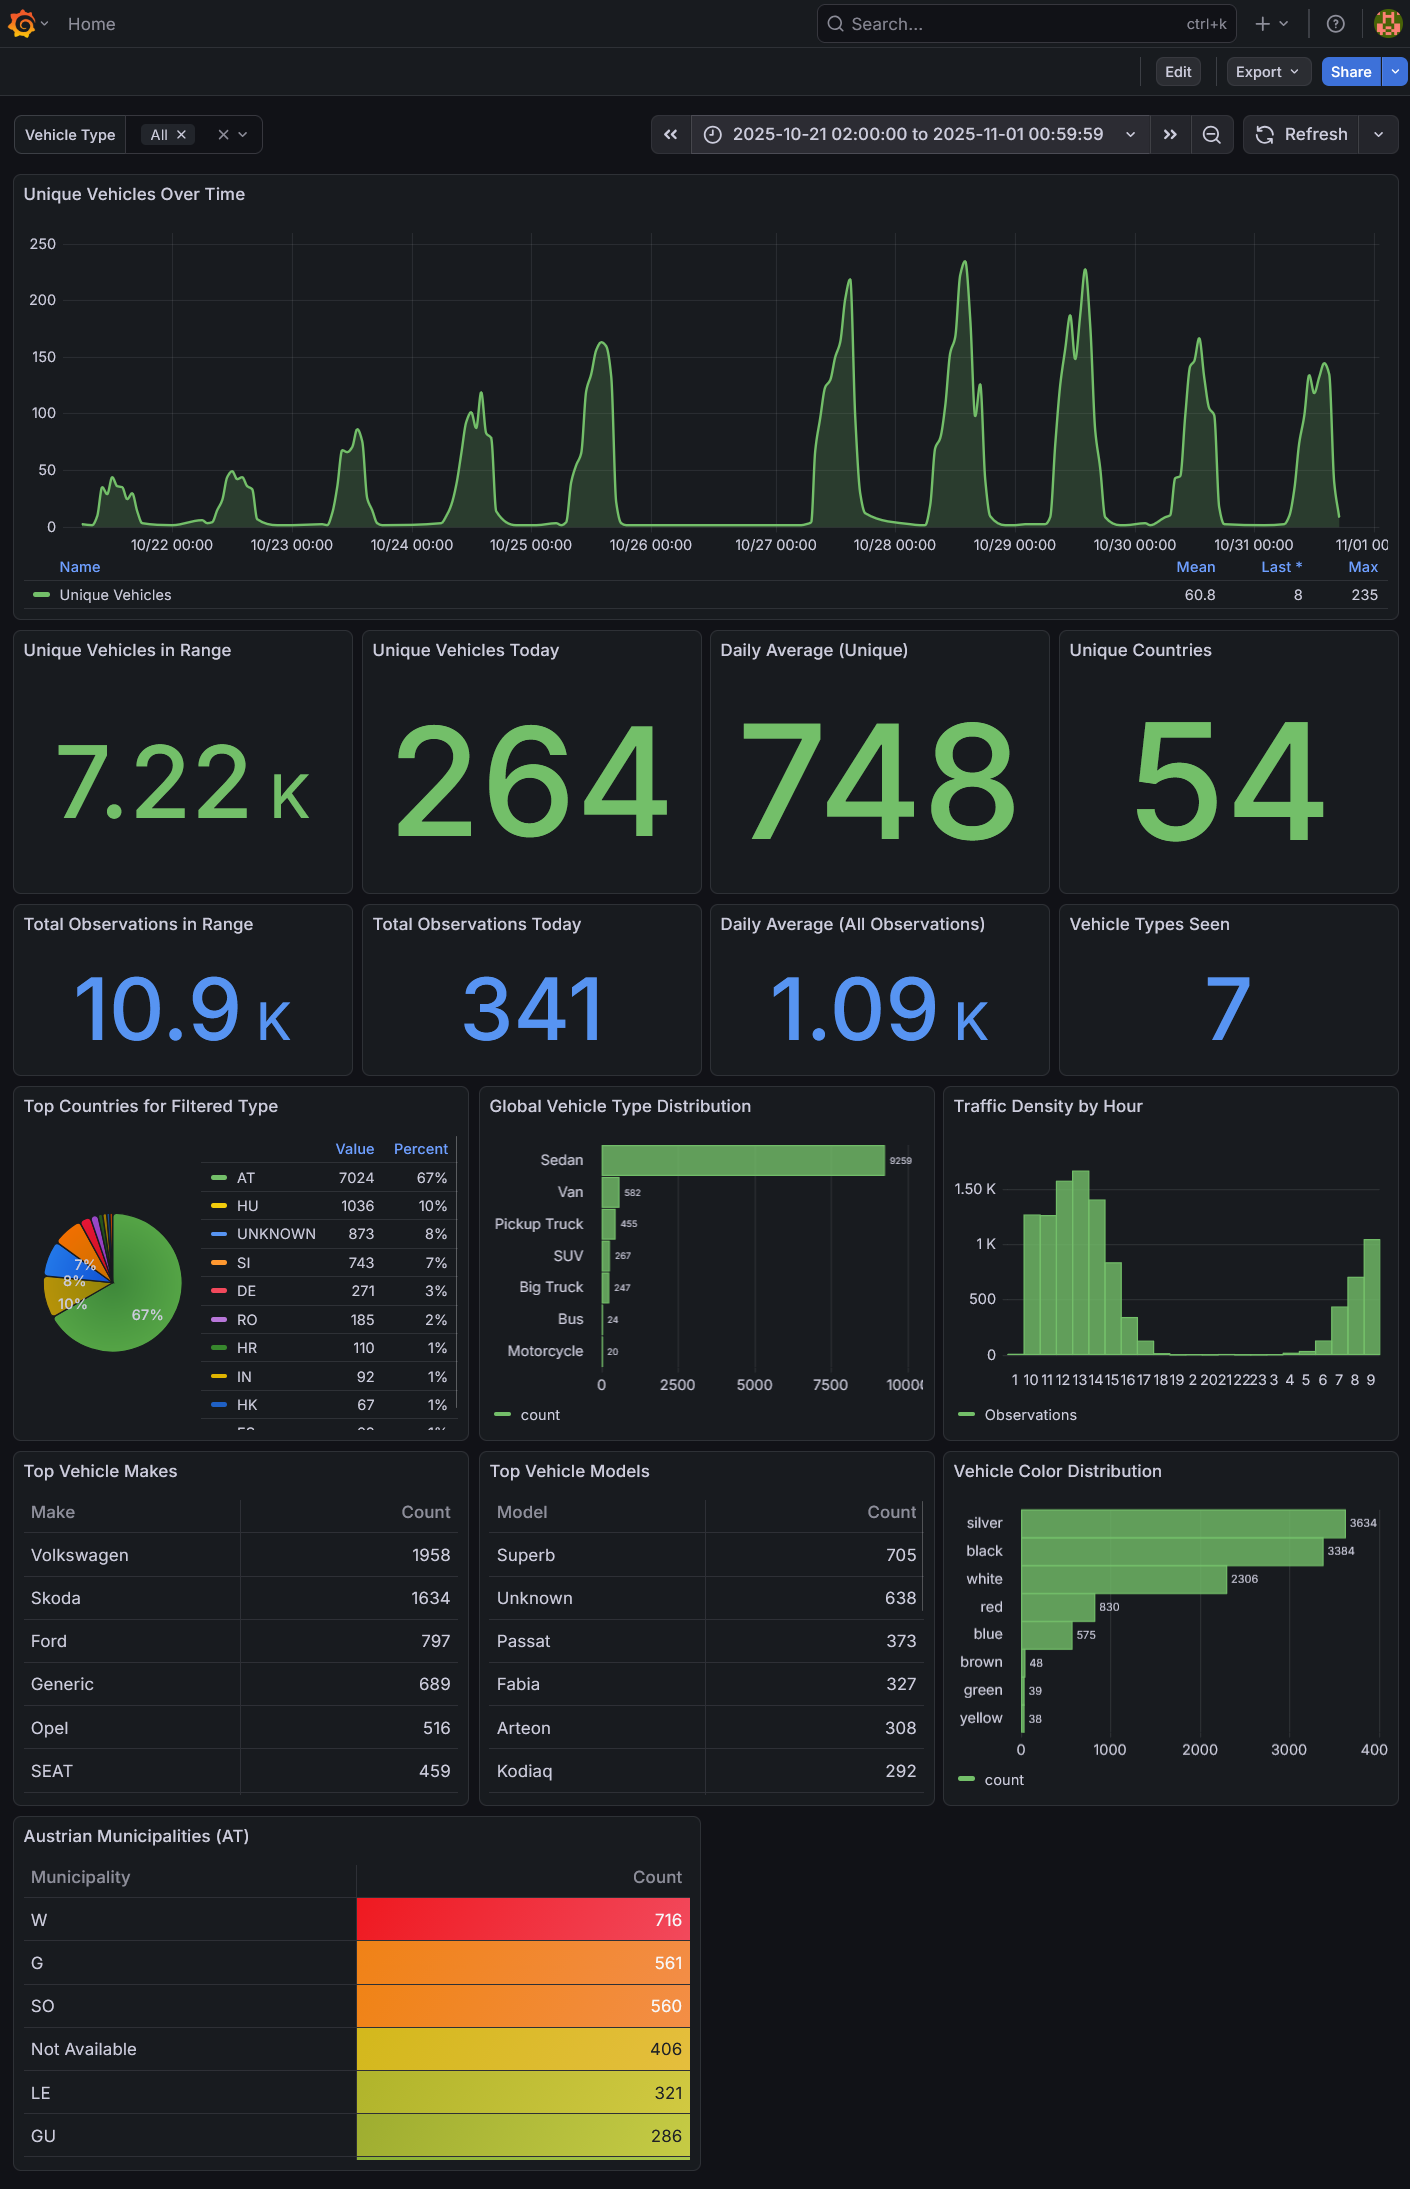
\includegraphics[width=0.9\textwidth]{grafana_dashboard.png}
    \caption{Grafana Dashboard}
    \label{fig:grafana_dashboard}
\end{figure}

\newpage

% Kapitel 6: Infrastruktur, Deployment und Betrieb
% Kapitel 6: Infrastruktur, Deployment und Betrieb
\section{Infrastruktur, Deployment und Betrieb}
\label{sec:infrastruktur}

Dieses Kapitel behandelt die infrastrukturellen Komponenten und Prozesse dieser Diplomarbeit.
Erläutert werden unter anderem der Deployment-Prozess sowie die im laufenden Betrieb relevanten Aspekte wie Monitoring und Logging, Datenbank-Management und Backup-Strategien.


\subsection{Container-Orchestrierung}
\label{sec:container_orchestrierung}

Die gesamte Applikation wird mittels Docker Compose orchestriert, wobei zwei separate Konfigurationsdateien für die Entwicklungs- und Produktionsumgebungen benutzt werden.
Docker Compose nutzt, wie bereits im entsprechenden Kapitel erwähnt, YAML-Dateien, welche zur Unterscheidung mit den Endungen \texttt{.prod.yaml} und \texttt{.dev.yaml} versehen wurden.
Beide Konfigurationen definieren dieselben Services, unterscheiden sich jedoch grundlegend in der Art und Weise, wie diese für Docker zum Starten bereitgestellt werden.


\subsubsection{Entwicklungsumgebung}

In der Entwicklungsumgebung werden alle Services lokal aus ihren jeweiligen Dockerfiles gebaut.
Ein zentrales Merkmal ist die Verwendung von Volume-Mounts, welche lokale Dateiverzeichnisse direkt in die Container einbinden:

\begin{lstlisting}[language=yaml, caption={Volume Mount Entwicklungs-Compose-Konfiguration}, label={lst:compose_dev}]
data-collection-service:
  build:
    context: ./services/data-collection-service
    dockerfile: Dockerfile
  volumes:
    - ./services/data-collection-service/src:/app/src:rw
\end{lstlisting}

Durch diese Konfiguration werden Codeänderungen sofort im laufenden Container wirksam (Hot-Reload), ohne dass der Container neu gebaut werden muss.
Dies beschleunigt den Entwicklungszyklus erheblich, da Änderungen am Quellcode schnell in der Docker-Umgebung getestet werden können.

\newpage
\subsubsection{Produktionsumgebung}

Die Produktionskonfiguration verwendet hingegen vorgefertigte Docker-Images, welche über eine Docker-Registry heruntergeladen werden:

\begin{lstlisting}[language=yaml, caption={Image Produktions-Compose-Konfiguration}, label={lst:compose_prod}]
data-collection-service:
  image: julianbierbaum/license-plate-system:data-collection-service
  restart: unless-stopped
\end{lstlisting}

Die Volume-Mounts für den Quellcode entfallen hier vollständig, da dieser direkt in die zuvor gebauten Images eingebettet wurde.
Eine wichtige Ausnahme hierbei ist allerdings das Volume der Datenbank, welches für den Bestand der Daten weiterhin außerhalb des Images gespeichert wird.
Dies bedeutet, dass diese Images eigenständig sind und alle Abhängigkeiten sowie den Applikationscode bereits enthalten.

Für das Deployment auf der Produktionsumgebung werden daher ausschließlich die Docker Compose-Datei und die Umgebungsvariablen zur Konfiguration benötigt, ein Klonen des Quellcode-Repositories ist nicht erforderlich.
Dies ist für die Nutzung von Portainer wichtig, ein Tool, welches später in diesem Kapitel näher beleuchtet wird.
Zusätzlich wurde die Restart-Policy strikter gesetzt, um sicherzustellen, dass Container nach einem Absturz oder einem Neustart des Host-Systems automatisch wieder hochgefahren werden.


\subsubsection{Startabhängigkeiten und Healthchecks}

Ein wesentlicher Aspekt der Orchestrierung ist die korrekte Startreihenfolge der Services.
Da alle Applikationsservices eine funktionierende Datenbank voraussetzen, wird ein spezieller Datenbank-Prestart-Container eingesetzt, welcher die Datenbank initial konfiguriert.
Erst wenn dieser Container erfolgreich durchgelaufen ist, werden die abhängigen Services gestartet:

\begin{lstlisting}[language=yaml, caption={Startabhängigkeiten Datenbank Prestart}, label={lst:compose_depends}]
depends_on:
  db-prestart:
    condition: service_completed_successfully
\end{lstlisting}

Der Prestart-Service wartet selbst wiederum auf den PostgreSQL-Container, welcher über einen Healthcheck seine Bereitschaft signalisiert.
Zusätzlich verfügen die Backend-Services und der Plate Recognizer-Container über eigene Healthchecks, mit welchen, über definierte HTTP-Endpunkte der aktuellen Zustand eines Services überwacht werden kann.

\newpage
\subsection{CI/CD Pipelines und Deployment}
\label{sec:cicd}

CI/CD (Continuous Integration / Continuous Delivery) bezeichnet die Praxis, Codeänderungen automatisiert zu testen, bauen und bereitzustellen \cite{redhat_cicd}.
Continuous Integration stellt sicher, dass Codeänderungen automatisch auf Fehler geprüft werden, bevor diese in den Hauptbranch des Code-Repositories aufgenommen werden.
Continuous Delivery automatisiert darauf aufbauend den Build- und Bereitstellungsprozess, sodass neue Versionen automatisch in der Docker-Registry als Images zur Verfügung gestellt werden.

Die Umsetzung dieser Prinzipien erfolgt im Projekt über GitHub Actions, ein in GitHub integriertes Automatisierungstool, mit welchem Workflows zum Bauen, Testen und Bereitstellen von Software direkt im Repository definiert werden können.
Diese Prozesse werden durch Ereignisse wie Code-Pushes oder Merges automatisch ausgelöst und führen die konfigurierten Schritte auf virtuellen Servern aus. \cite{github_actions}

\subsubsection{Build und Test Pipeline}

Die primäre CI/CD-Pipeline wird bei jedem Push auf einen beliebigen Branch ausgelöst und besteht aus zwei sequenziellen Phasen:

\paragraph{Phase 1: Testing und Linting}
In der ersten Phase werden für jeden Python-Service automatisiert drei Prüfungen durchgeführt:

\begin{enumerate}
  \item Formatierung (Ruff Format \cite{ruff_formatter}): Überprüfung des Codes auf Einhaltung der definierten Formatierungsregeln.
  \item Linting (Ruff Check \cite{ruff_linter}): Statische Codeanalyse zur Erkennung von potenziellen Fehlern und Stilabweichungen.
  \item Tests (Pytest mit Coverage): Ausführung aller Test-Cases, welche mit einer Codeabdeckungsanalyse kombiniert werden.
\end{enumerate}

Alle Tests werden innerhalb von Docker-Containern ausgeführt, um eine konsistente und reproduzierbare Testumgebung zu gewährleisten, welche der Produktionsumgebung möglichst nahekommt.

\newpage
\paragraph{Phase 2: Build und Push}
Wenn die Testphase erfolgreich abgeschlossen wurde und der Push auf dem Haupt-Branch erfolgt, wird die zweite Phase ausgelöst.
Diese nutzt ein Build-Script, welches automatisiert alle Docker-Images baut und in die definierte Registry pusht.

\begin{lstlisting}[language=bash, caption={Auszug Build-Script \texttt{build.sh}}, label={lst:build_script}]
# Build all services
for SERVICE_DIR in services/*/; do
  SERVICE_NAME=$(basename "$SERVICE_DIR")
  echo "--- Building ${SERVICE_NAME} ---"

  # Check Python lock file
  if [ -f "${SERVICE_DIR}pyproject.toml" ] && [ ! -f "${SERVICE_DIR}uv.lock" ]; then
    echo "Error: ${SERVICE_DIR}uv.lock not found. Run uv sync first."
    exit 1
  fi

  # Check Node.js lock file
  if [ -f "${SERVICE_DIR}package.json" ] && [ ! -f "${SERVICE_DIR}package-lock.json" ]; then
    echo "Error: ${SERVICE_DIR}package-lock.json not found. Run npm install first."
    exit 1
  fi

  docker build -t "${DOCKER_REGISTRY}:${SERVICE_NAME}" "$SERVICE_DIR"
  docker push "${DOCKER_REGISTRY}:${SERVICE_NAME}"
done
\end{lstlisting}

Dieses iteriert, wie im Code-Ausschnitt zu sehen ist, über alle Service-Verzeichnisse und identifiziert dabei Services anhand ihrer Lock-Files.
Da für die Python-Services UV als Package Manager benutzt wurde, dient das \texttt{uv.lock}-File als Identifikationsmerkmal für diese.
Frontend-Services werden mittels des \texttt{package-lock.json}-Files identifiziert und alle anderen Services, welche nicht im Service-Verzeichnis liegen, werden separat aufgerufen.
Das vollständige \texttt{build.sh}-Script ist im Anhang einsehbar.

\newpage
\subsubsection{Deployment mit Portainer}

Deployment auf der Produktionsumgebung erfolgt über die Plattform Portainer, ein Container Management-Tool mit Weboberfläche \cite{portainer}.
Portainer wurde auf dem Synology-NAS installiert und ermöglicht das Verwalten der Docker-Container direkt über einen Browser.

Für das Deployment wird in Portainer ein Stack erstellt, welcher die Produktions-Compose-Datei sowie die Datei mit den Umgebungsvariablen enthält.
Bei Aktualisierungen werden die neuesten Images aus dem Docker-Registry heruntergeladen, woraufhin die betroffenen Container automatisch neu erstellt werden, ohne dass die Datenhaltung betroffen ist.

\begin{figure}[htbp]
  \centering
  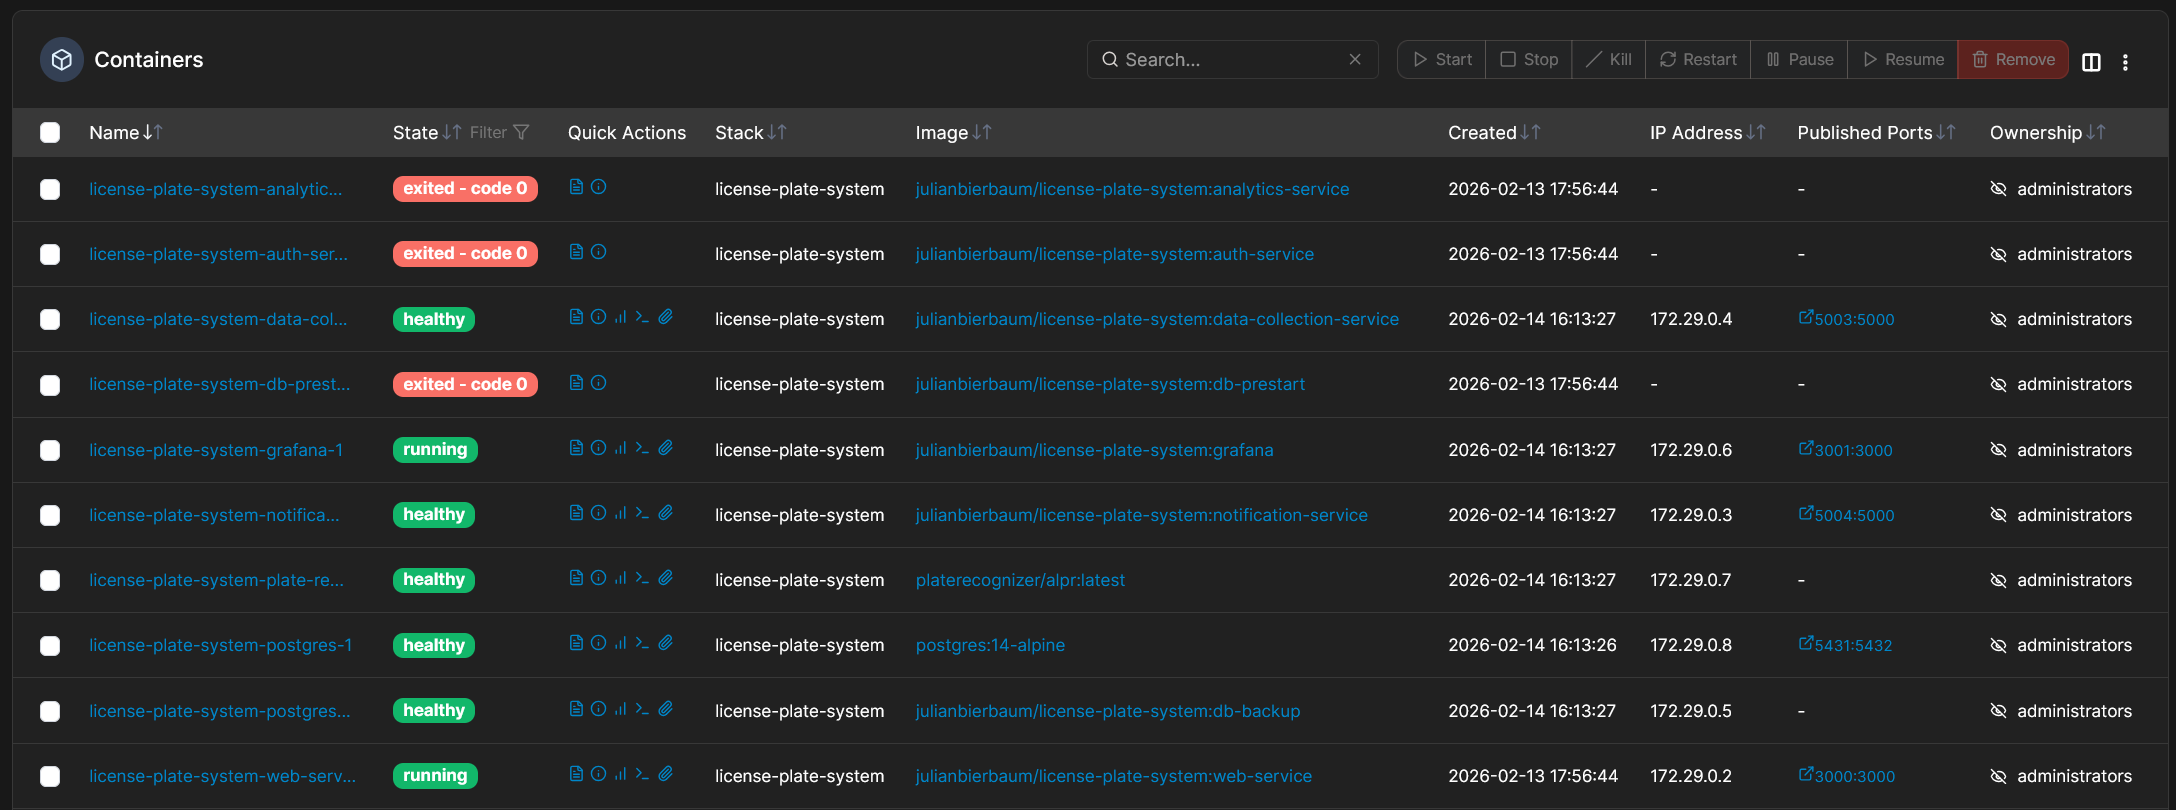
\includegraphics[width=\textwidth]{container_stack_portainer.png}
  \caption{Laufender Container-Stack in Portainer}
  \label{fig:portainer}
\end{figure}

\newpage
\subsection{Monitoring und Logging}


\subsubsection{Healthchecks}

Wie bereits erwähnt (Kapitel~\ref{sec:container_orchestrierung}) verfügen die Services über Healthchecks, welche von Docker Compose in regelmäßigen Intervallen (alle 5 Sekunden) ausgeführt werden und primär dazu dienen, die Verfügbarkeit der Services zu überwachen.
Die Methode des Healthchecks variiert je nach Service-Art:

\begin{itemize}
  \item Backend-Services (Data Collection, Notification): HTTP-Request an den \texttt{/health}-Endpunkt des jeweiligen Services.
  \item PostgreSQL-Datenbank: Verwendung des nativen \texttt{pg\_isready}-Kommandos zur Überprüfung der Datenbankbereitschaft.
  \item Plate Recognizer: HTTP-Request an den Root-Endpunkt des ALPR-Containers.
  \item Backup-Service: Überprüfung, ob der Cron-Daemon (\texttt{crond}) als Prozess läuft.
\end{itemize}

Der Status der Healthchecks ist über Portainer einsehbar und ermöglicht somit eine zentrale Überwachung des Status aller Container.


\subsubsection{Logging}

Alle Services wurden so konfiguriert, dass Log-Ausgaben direkt auf die Konsole geschrieben werden (Console-Logging).
Das Log-Level ist über eine Umgebungsvariable konfigurierbar und wird in der Produktionsumgebung typischerweise auf INFO gesetzt, während in der Entwicklungsumgebung DEBUG als Standard dient.

Die Logs sind über Docker und Portainer einsehbar.
Durch die Verwendung des Python Logging-Moduls in allen Backend-Services wird ein einheitliches Log-Format erzeugt, welches Zeitstempel, Log-Level und den Namen des Services enthält, auf welchem der Log erstellt wurde.

\begin{lstlisting}[caption={Beispielhafte Log-Ausgabe des Data Collection Services}, label={lst:log_example}]
2026-02-17 15:55:24,782 - data-collection-service - INFO - Vehicle detected from camera: BC500-001
2026-02-17 15:55:26,461 - data-collection-service - INFO - No vehicle observations found in reader result.
\end{lstlisting}

Des Weiteren könnte dieses Modul zukünftig erweitert werden, um etwa gleichzeitig mit dem Console-Log in zentrale Log-Files zu schreiben.

\newpage
\subsection{Datenbank-Management}


\subsubsection{Initiale Einrichtung}

Die initiale Einrichtung der Datenbank erfolgt automatisch beim ersten Start des Systems über den DB-Prestart-Container.
Dieser führt ein Entrypoint-Script aus, das zwei Aufgaben erfüllt:
Zunächst führt dieser ein Init-Script aus. Dieses SQL-Script erstellt die spezifischen Datenbank-Schemas und -Benutzer der Services, welche bereits im Kapitel~\ref{sec:db_architektur} erläutert wurden.
Zudem werden die granularen Berechtigungen vergeben, wie sie im Sicherheitskonzept (Abschnitt~\ref{sec:db_zugriff}) definiert wurden, beispielsweise erhält der Analytics-Service-User nur Leserechte auf das Ingestion-Schema.

Die zweite Aufgabe dieses Services ist die Ausführung der Datenbankmigrationen unter Benutzung von Alembic.
Nach der zuvor erwähnten Schema-Erstellung werden automatisch alle ausstehenden Migrationen angewendet, um die Tabellen in den aktuellen Zustand zu bringen.
Durch diese automatisierte Einrichtung entfällt jegliche manuelle Datenbankadministration beim initialen Deployment oder beim Neuaufsetzen des Systems.

Das init.sql-Script ist im Anhang angeführt.


\subsubsection{Schema-Migrationen mit Alembic}

Für die Versionierung des Datenbankschemas wird Alembic eingesetzt, ein Migrationswerkzeug für SQLAlchemy-basierte Anwendungen.

Der DB-Prestart-Container kopiert die SQLAlchemy-Modelle der einzelnen Services in den eigenen Build-Kontext und kann somit das Schema aller Services zentral verwalten. \cite{alembic_monorepo}
Diese sind mittels Volumes aus den Verzeichnissen der Backend-Services an den Prestart-Container angebunden.

\begin{lstlisting}[language=bash, caption={Dockerfile COPY Anweisungen}, label={lst:prestart_copy}]
COPY services/data-collection-service/src/ /app/data_collection/src/
COPY services/notification-service/src/ /app/notification/src/
# COPY services/analytics-service/src/ /app/analytics/src/
\end{lstlisting}

\newpage
Die Alembic-Konfiguration importiert die Base-Klassen der Backend-Services im Environment-Python-File:

\begin{lstlisting}[language=python, caption={Alembic target\_metadata}, label={lst:alembic_env}]
# Import Base objects
from data_collection.src.models.base import IngestionBase
from notification.src.models.base import NotificationBase
# from analytics.src.models.base import AnalyticsBase

target_metadata = [
    IngestionBase.metadata,
    NotificationBase.metadata,
    # AnalyticsBase.metadata,
]
\end{lstlisting}

Durch diesen zentralisierten Ansatz können Migrationen generiert werden, welche über alle Schemas hinweg konsistent sind.
Die Migrationen werden wie bei Alembic üblich versioniert und mit dem Repository eingecheckt, wobei jede Migration durch eine Python-Datei repräsentiert wird, welche sowohl die Up- als auch Downgrade-Funktion enthält, um Schema-Änderungen vorwärts und rückwärts anwenden zu können.

\newpage
\subsection{Backup-Strategie}

Die Backup-Strategie des Systems umfasst sowohl automatisierte als auch manuelle Sicherungsmechanismen und einen manuellen Wiederherstellungsprozess.


\subsubsection{Automatisiertes Backup}

Für die automatisierte Sicherung der PostgreSQL-Datenbank wird ein dedizierter Backup-Container eingesetzt, welcher als separater Service im Docker Compose-Stack definiert wurde.
Dieser Container basiert auf dem offiziellen PostgreSQL-Alpine-Image und nutzt den Cron-Daemon zur zeitgesteuerten Ausführung des Backup-Scripts.

Der Backup-Zeitplan wird über die Umgebungsvariable \texttt{BACKUP\_SCHEDULE} im Cron-Format konfiguriert (In diesem Fall etwa \texttt{0 2 * * *} für ein tägliches Backup um 02:00 Uhr \cite{cron_guru}).
Falls die Variable nicht gesetzt wurde, werden automatische Backups deaktiviert und der Container wechselt in einen Idle-Zustand.

\begin{figure}[htbp]
  \centering
  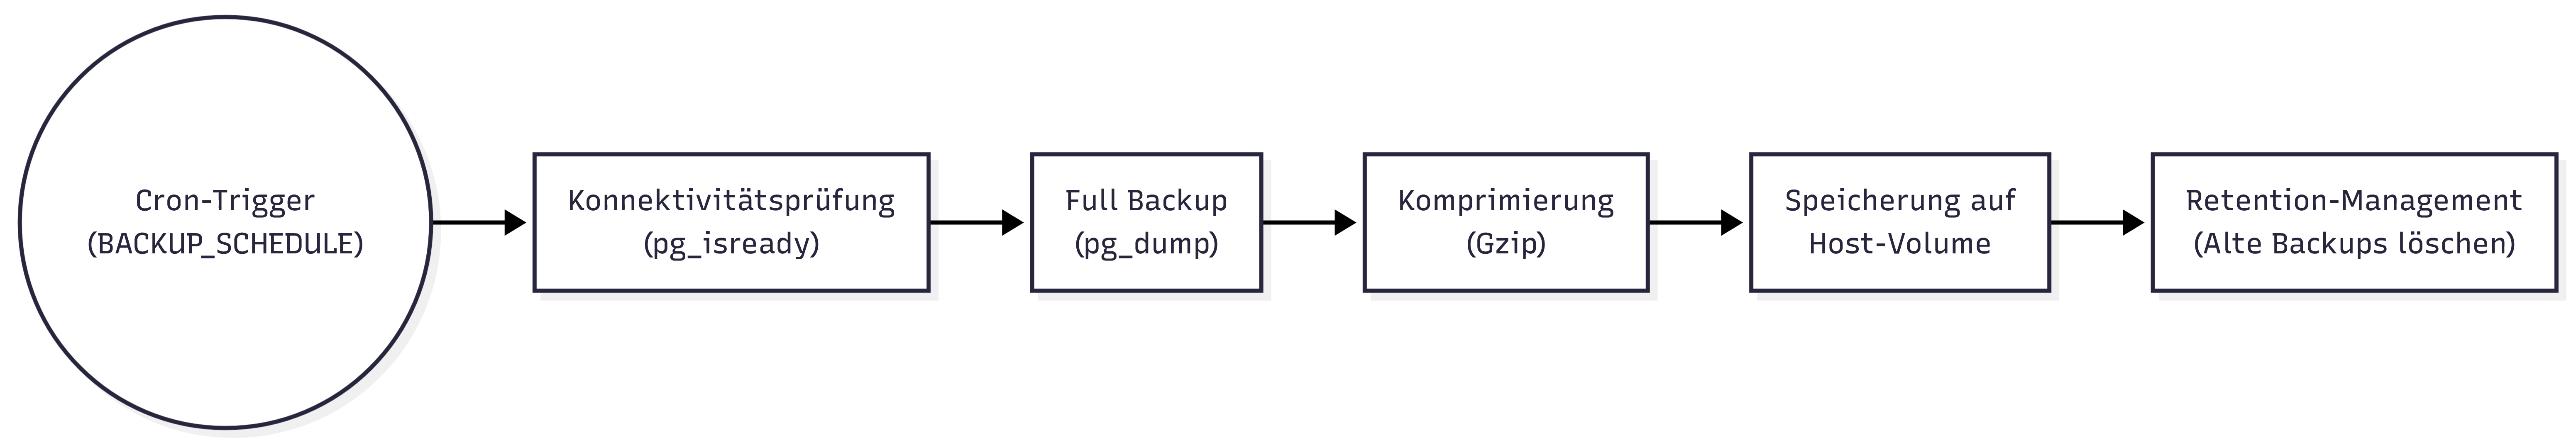
\includegraphics[width=\textwidth]{backup_flow.png}
  \caption{Backup Flow}
  \label{fig:backup_flow}
\end{figure}

Der Cron-Daemon löst das Backup-Script zum konfigurierten Zeitpunkt aus.
Dieses wartet zunächst auf die Erreichbarkeit der Datenbank, erstellt dann einen vollständigen Datenbank-Dump mittels \texttt{pg\_dump} \cite{postgres_pgdump}, komprimiert anschließend diesen mit Gzip und schreibt die entstandene Backup-Datei auf ein gemountetes Host-Volume.
Abschließend werden Backups, die älter als die konfigurierte Aufbewahrungsdauer (standardmäßig 30 Tage) sind, automatisch gelöscht.

In dieser Implementierung wird bei jedem Durchlauf ein vollständiges Datenbank-Backup (Full Backup) erstellt, anstatt auf inkrementelle oder differentielle Strategien zurückzugreifen.
Wie im Kapitel zur Datenbankarchitektur (\ref{sec:denormalisierung}) errechnet, beträgt die Größe eines komprimierten Full-Backups selbst bei über 60.000 gespeicherten Erkennungen lediglich rund 3,4 MB.
Bei diesen Größenordnungen bringt eine inkrementelle Strategie keinen nennenswerten Vorteil, würde jedoch die Komplexität der Wiederherstellung erhöhen, da inkrementelle Backups stets auf einem vollständigen Basis-Backup aufbauen und in korrekter Reihenfolge eingespielt werden müssen.


\subsubsection{Manuelles Backup und Wiederherstellung}

Zusätzlich zu den automatisierten Backups steht ein manuelles Backup-Script zur Verfügung.
Dieses startet einen temporären PostgreSQL-Container, der den Dump erstellt und anschließend sofort wieder entfernt wird.
Ansonsten ist dieser funktionell gleich aufgebaut, wie das oben aufgezeigte System für automatisierte Backups.

Für die Wiederherstellung existiert ebenfalls ein Script, welches einen vollständigen Disaster-Recovery-Prozess implementiert:

\begin{figure}[htbp]
  \centering
  
\includegraphics[width=1.1\textwidth]{restore_flow.png}
  \caption{Restore Flow}
  \label{fig:restore_flow}
\end{figure}

Das Script fordert zunächst eine explizite Bestätigung, da alle in der Datenbank bestehenden Daten überschrieben werden müssen.
Anschließend werden alle aktiven Datenbankverbindungen terminiert, die bestehende Datenbank gelöscht und neu angelegt, bevor das komprimierte Backup mittels \texttt{pg\_restore} \cite{postgres_pgrestore} eingespielt wird.

Das Recovery Point Objective (RPO) entspricht dem konfigurierten Backup-Intervall (standardmäßig 24 Stunden), das Recovery Time Objective (RTO) beträgt einige Sekunden bis wenige Minuten und ist primär durch die Größe des Backups bestimmt.

\subsection{Documentation as Code (MkDocs)}

Die Entwicklerdokumentation wird im Repository gepflegt und automatisiert, mithilfe von GitHub Pages \cite{github_pages}, veröffentlicht.
Hierfür wird MkDocs \cite{mkdocs} mit dem Material-Theme \cite{mkdocs_material} eingesetzt, ein Python-basierter Static-Site-Generator, welcher Markdown-Dateien in eine Dokumentationswebsite transformiert.
Die Verwendung von MkDocs hat den Vorteil, dass out-of-the-box viele Grundfunktionen einer guten Dokumentation, wie etwa eine Navigationsleiste oder Suchfunktion, bereits als Module funktionsfähig bereitgestellt werden.

Die Dokumentation ist in sechs Hauptbereiche gegliedert:
\begin{itemize}
  \item Getting Started Voraussetzungen, Installation und Konfiguration für neue Entwickler
  \item Development: Entwicklungsumgebung, Docker-Befehle und Service-Entwicklung
  \item Operations: Backup-Verfahren, Wiederherstellung und Monitoring
  \item Deployment: Übersicht, Image-Erstellung und Produktionseinrichtung
  \item Reference: Script-Referenzen, Docker-Compose-Dokumentation, API-Dokumentation und Data-Collection-Flow
\end{itemize}

Die Veröffentlichung von Änderungen erfolgt automatisiert über einen eigenen GitHub-Actions-Workflow.
Im Falle eines Pushes wird die Dokumentation neu gebaut und auf GitHub Pages veröffentlicht.
Dadurch ist die Dokumentation stets synchron mit dem aktuellen Stand des Codes und unter einer permanenten, öffentlichen URL erreichbar.

Dieser Ansatz folgt dem Documentation-as-Code-Prinzip, bedeutet, dass die Dokumentation derselben Versionskontrolle wie der Quellcode unterliegt und Änderungen denselben Review-Prozess (Pull Requests) durchlaufen.
Dies hat in der Entwicklung den großen Vorteil, dass die Dokumentation als Teil der Code-Basis gesehen und verwaltet wird und so einfacher und schneller bei Änderungen angepasst werden kann.

\begin{figure}[htbp]
  \centering
  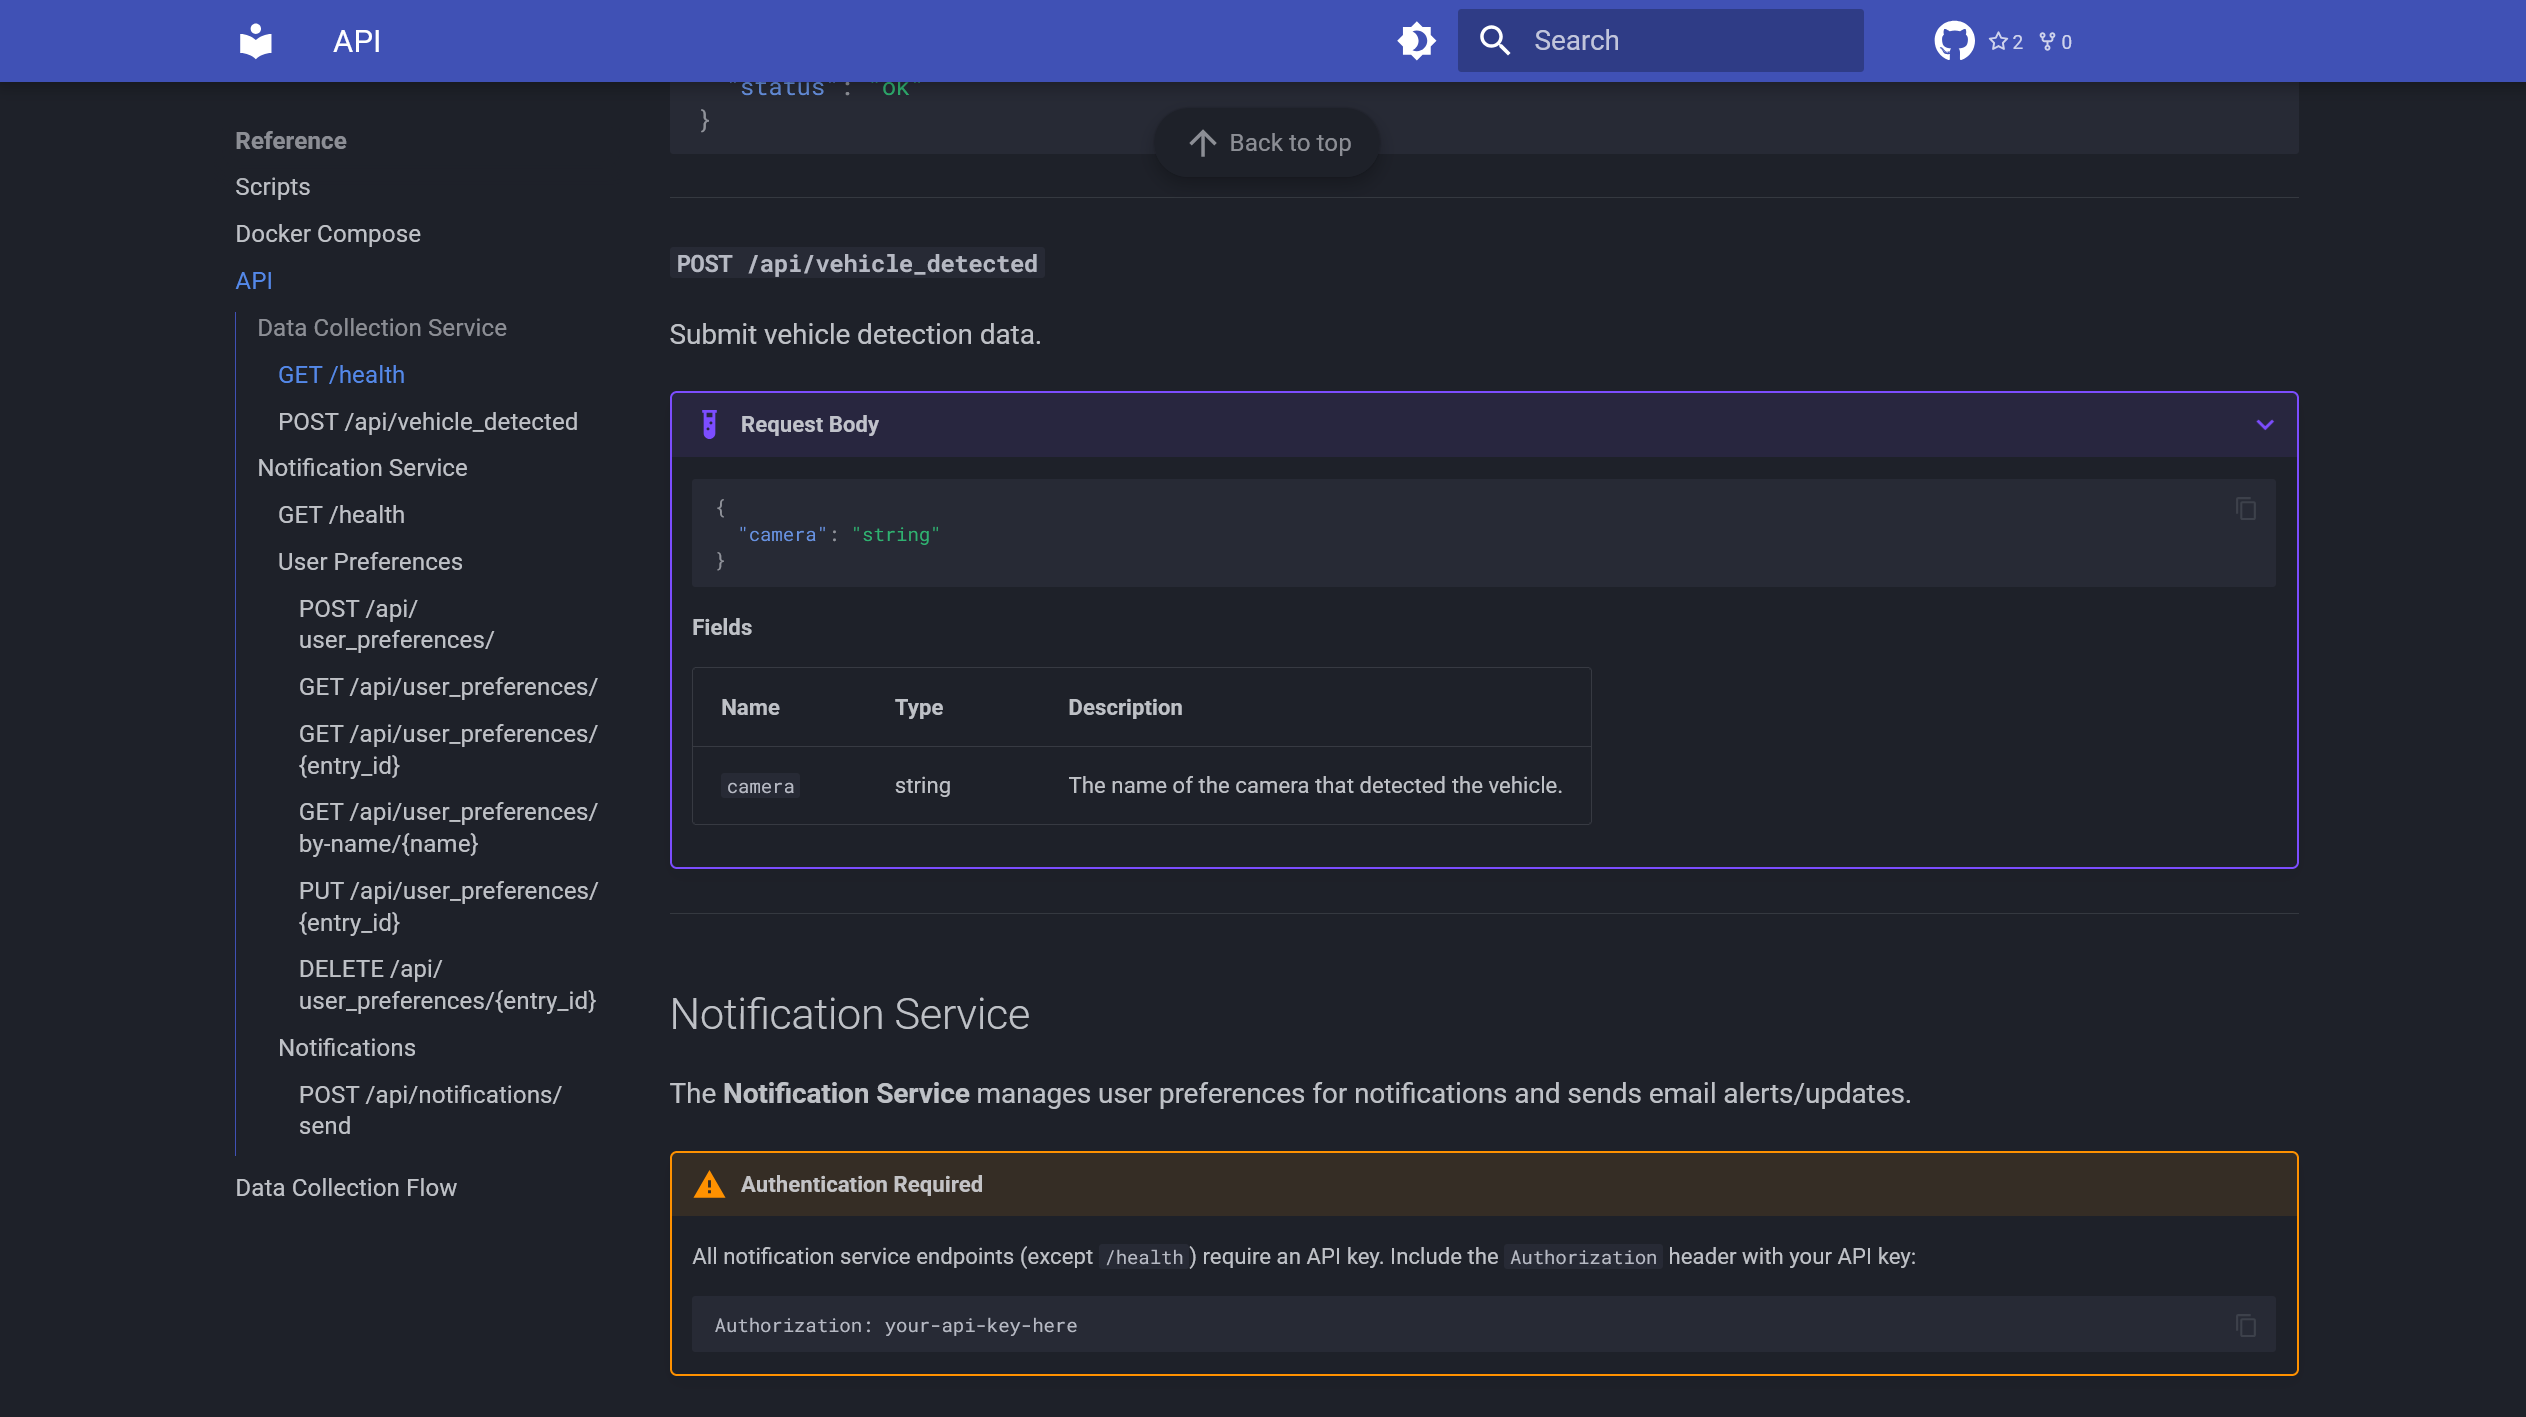
\includegraphics[width=\textwidth]{mkdocs.png}
  \caption{Entwicklerdokumentation mittels MkDocs}
  \label{fig:mkdocs}
\end{figure}

\newpage

% Kapitel 7: Qualitätssicherung und Tests
% Kapitel 7: Qualitätssicherung und Tests
\section{Qualitätssicherung und Tests}
\label{sec:qualitaetssicherung}

Das folgende Kapitel beschreibt die Maßnahmen zur Sicherstellung der Softwarequalität sowie die Bewertung der Qualität des Gesamtsystems unter realen Einsatzbedingungen.


\subsection{Teststrategie}

Die Teststrategie des Projekts kombiniert Unit-Tests zur Überprüfung einzelner Komponenten mit Integrationstests, welche das Zusammenspiel der Services auf API-Ebene validieren.
Als Test-Framework wird Pytest \cite{pytest} eingesetzt, ergänzt durch das Pytest-Coverage-Modul \cite{pytest_cov} für Codeabdeckungsanalysen.
Hierbei wurde das Ziel festgelegt, eine Testabdeckung von über 90\% für jeden Python-Service zu erreichen. \\
Dies konnte in der Implementierung mit einer Testabdeckung von 91\% für den Data-Collection Service und 94\% für den Notification Service auch erreicht werden.


\subsubsection{Unit-Tests}

Die Unit-Tests decken die Handler-Klassen beider Python-Services ab und sind nach dem Arrange-Act-Assert-Pattern (AAA) strukturiert.
Externe Abhängigkeiten wie die Synology-API, Plate Recognizer und der SMTP-Server werden durch die Mocking-Library \texttt{unittest.mock} simuliert, um die Tests unabhängig von externen Services ausführbar zu machen.

Im Data Collection Service werden alle vier Handler-Klassen einzeln getestet:

\begin{itemize}
    \item \textbf{CameraHandler:}
          Tests, welche die Interaktion mit der Synology-API durch gemockte HTTP-Responses simulieren.
          Dies umfasst Erfolgs- und Fehlerszenarien für Authentifizierung, Kameraabruf und Snapshot-Erstellung.

    \item \textbf{PlateRecognizerHandler:}
          Tests für den ALPR-API-Aufruf, geprüft mit gemockten HTTP-Responses für erfolgreiche und fehlgeschlagene Anfragen.

    \item \textbf{CountryHandler:}
          Die Bezirkserkennung für österreichische und slowenische Kennzeichen mit verschiedenen Eingabekombinationen wird mit Tests überprüft (z.B. unbekannter Ländercode, ein- und zweibuchstabige Kürzel).

    \item \textbf{DatabaseHandler:}
          Tests für Datenextraktion aus API-Antworten, Hash-Normalisierung (Groß-/Kleinschreibung, Leerzeichen) und die zeitfensterbasierte Duplikatserkennung mit Datenbankinteraktionen.
\end{itemize}

\newpage
Im Notification Service werden ebenfalls die Handler und Datenbankschicht getestet:

\begin{itemize}
    \item \textbf{EmailHandler:}
          Tests für den SMTP-Versand mit gemocktem SMTP-Server, Bulk-Versand mit teilweisen Fehlern sowie der korrekte Versand von Alert- und Update-E-Mails.

    \item \textbf{DatabaseHandler:}
          CRUD-Operationen für Benutzerpräferenzen, einschließlich Duplikat-E-Mail-Erkennung und Filterung nach Benachrichtigungspräferenzen.
\end{itemize}


\subsubsection{Integrationstests}

Die Integrationstests überprüfen die vollständigen API-Endpunkte unter Verwendung von FastAPI.
Dieses ermöglicht das Senden von HTTP-Requests gegen die Applikation, ohne einen externen Server starten zu müssen.

Für den Notification Service umfasst dies die vollständige CRUD-Schnittstelle der Benutzerpräferenzen (Create, Read, Update, Delete) sowie die Benachrichtigungs-API mit verschiedenen Empfänger-Szenarien (alle Abonnenten, spezifische Empfänger, keine Empfänger, Zustellfehler).


\subsubsection{Testisolation und Datenbankstrategie}

Die Tests werden innerhalb der CI-Pipeline mit den zugehörigen Service-Containern gegen den PostgreSQL-Service ausgeführt, anstatt eine In-Memory-Datenbank wie SQLite als Ersatz zu verwenden.
Diese Entscheidung wurde getroffen, da SQLite wesentliche benutzte PostgreSQL-Funktionalitäten nicht identisch abbilden kann.
Beispiele hierfür sind die Verwendung des nativen PostgreSQL-Enum-Datentyps \cite{postgresql_enum} für die Fahrzeugorientierung sowie die Verwendung von zeitzonenbehafteten Zeitstempeln \cite{postgresql_datetime}.
SQLite bietet für diese Typen keine native Unterstützung \cite{sqlite_datatypes}.
Durch die Nutzung derselben Datenbank-Engine in den Tests wird sichergestellt, dass die Tests tatsächlich das Verhalten der Produktionsumgebung widerspiegeln und keine falsch-positiven Ergebnisse durch abweichendes Datenbankverhalten entstehen.

\newpage
Beide dieser Services verwenden ein identisches Muster zur Datenisolation in ihrer Pytest-Konfigurationsdatei:

\begin{lstlisting}[language=Python, caption={Pytest-Fixture für Datenisolation}, label={lst:conftest}]
@pytest.fixture(scope='function')
def db():
    """
    Provides a SQLAlchemy session for each test function.
    Each test will run within its own transaction, which is 
    then rolled back at the end of the test, ensuring data 
    isolation without dropping tables.
    """
    connection = test_engine.connect()
    transaction = connection.begin()
    session = TestingSessionLocal(bind=connection)

    try:
        yield session
    finally:
        session.close()
        transaction.rollback()
        connection.close()
\end{lstlisting}

Jeder Test wird innerhalb einer eigenen Datenbank-Transaktion ausgeführt, die nach dem Test automatisch zurückgerollt wird.
Dadurch werden alle Datenbankänderungen eines Tests nach dessen Abschluss verworfen und die Tests beeinflussen sich gegenseitig nicht.
Die Reihenfolge der Testausführung ist somit beliebig.

Für die Integrationstests wird zusätzlich die FastAPI Dependency-Injection überschrieben, sodass der Test-Client die Test-Datenbanksession und, im Fall des Notification Service, einen Test-API-Key verwendet.

\newpage
\subsection{Qualitätssicherung der Kennzeichenerkennung}
\label{sec:qs_alpr}

Die Bewertung der Erkennungsrate in einem ALPR-System wird dadurch erschwert, dass eine exakte Dunkelziffer, also der Anteil der Fahrzeuge, welche das System passieren aber nicht erkannt werden, ohne eine unabhängige Referenzmessung nicht ermittelt werden kann.
Eine systematische Gegenüberstellung jeder einzelnen physischen Durchfahrt mit der entsprechenden Systemerkennung wurde im Rahmen dieser Arbeit nicht durchgeführt.
Dies begründet sich dadurch, dass eine bloße Erfassung der Fahrzeuganzahl ohne erfolgreiche Kennzeichenidentifikation einen geringen operativen Zusatznutzen bieten würde, da die eigentliche Relevanz der Daten in der Analyse von Trends und statistischen Mittelwerten liegt.
Die folgenden Erkenntnisse basieren daher auf Beobachtungen während des Betriebszeitraums sowie auf der Analyse der gespeicherten Erkennungsdaten.

\subsubsection{Herausforderungen und Umgebungseinflüsse}

Mehrere Umgebungsfaktoren beeinflussen die Erkennungsqualität im täglichen Betrieb maßgeblich:

\begin{itemize}
    \item \textbf{Lichtverhältnisse:} Da die Zufahrt nach Süden ausgerichtet ist, ergeben sich bei tiefem Sonnenstand (insbesondere in den Morgen- und Abendstunden sowie im Winter) Gegenlichtbedingungen, welche die Kennzeichenlesbarkeit beeinträchtigen können.
    \item \textbf{Witterungseinflüsse:} Bei starkem Regen, Schneefall oder Nebel ist mit einer reduzierten Erkennungsrate zu rechnen, da die Sichtbarkeit der Kennzeichen physisch eingeschränkt ist.
    \item \textbf{Nachtbetrieb:} Nächtliche Erkennungen profitieren von der integrierten Infrarot-Beleuchtung der Kamera, die Kennzeichen auch bei vollständiger Dunkelheit ausreichend beleuchtet und lesbar macht.
\end{itemize}

\newpage
\subsubsection{Implementierte Maßnahmen zur Datenoptimierung}

Zur Sicherung der Datenqualität im Praxisbetrieb wurden zwei zentrale Strategien angewandt, um Fehlinterpretationen und Datenredundanz zu minimieren:

\paragraph{Zeitfensterbasierte Duplikatserkennung}
Wie in Abschnitt~\ref{sec:duplikatpruefung} beschrieben, verhindert ein konfigurierbarer Intervall-Filter Mehrfacherkennungen desselben Fahrzeugs (z. B. bei langsamer Durchfahrt oder kurzem Stopp im Erkennungsbereich). Dies stellt sicher, dass ein Fahrzeug innerhalb eines logischen Zeitrahmens nur einmal gewertet wird.

\paragraph{Regionale Einschränkung (Ländercodes)}
Die ALPR-Analyse wurde gezielt auf die vier relevanten Länder (AT, HU, SI, DE) beschränkt. Dies verbessert die Genauigkeit signifikant, da das Modell länderspezifische Kennzeichenformate priorisiert und so die Wahrscheinlichkeit von Verwechslungen bei ähnlichen Schriftarten verringert.

Durch diese kombinierten Maßnahmen wird eine für den statistischen Anwendungszweck ausreichend hohe Datenqualität erreicht, welche die beschriebenen physikalischen Limitationen der optischen Erkennung effektiv kompensiert.
\newpage

% Kapitel 8: Fazit und Ausblick
\input{./../02a_DOC_DPL1/kap_08_fazit_ausblick.tex}

%
%****************************************************************************************************
%============================= E N D   S U B D O C U M E N T  ==========================
%****************************************************************************************************
%
\end{document}
